
\documentclass[a4paper,12pt]{report}
\usepackage{a4wide}

%\documentclass[a5paper,10pt]{book}
%\usepackage[top=23mm, bottom=18mm, left=15mm, right=25mm]{geometry}
%\geometry{papersize={170mm,220mm}}


\usepackage[utf8x]{inputenc}
\usepackage[danish]{babel}

\usepackage{xr-hyper} %Externe hyper-ref
\usepackage[colorlinks=true, hyperindex=true, linkcolor=minmblaa, citecolor=minmblaa, urlcolor=minmblaa]{hyperref}
\hypersetup{colorlinks=true,filecolor=minmblaa,bookmarksnumbered=true} %Til hyperreferencer. Referencer med farver
\usepackage{needspace} % giver mulighed for at kræve at der skal være et antal tomme linier på siden før ellers indsættes et sideskift.
\usepackage{framed} %Bokse
\usepackage{wrapfig}

\usepackage{amsmath,amsfonts,amssymb,amsthm,mathtools} %Matematikpakker

\setlength{\parindent}{0mm} %Ingen Indhak i første linje i afsnit

\usepackage{color} %Farvepakke

\usepackage{array}
\usepackage{colortbl}
\usepackage{multirow} %Til at flette rækker i tabeller.

\usepackage{verbatim,mhchem}



	% DOWNLOAD FRA: http://sarovar.org/frs/?group_id=52&release_id=97
	% Læg i directory for hoved TEX fil
%\usepackage[draft]{pdfdraftcopy}
%\draftstring{Licens: Kasper Langt Mellemnavn Skårhøj}
%\draftfontsize{30}
	%\draftfontfamily{hlh}
	%\draftangle{45}
	%\definecolor{mycolor}{rgb}{.825,.855,1}
	%\draftcolor{mycolor}
	%\draftfontattrib



% = Sidehoved =
\usepackage{fancyhdr}
\pagestyle{fancy}
\renewcommand{\sectionmark}[1]{\markright{\protect\titlegraphic{dturoed}\textcolor{dtugraa}{\thesection~\MakeUppercase{#1}}}} % \thesection.\
\fancyhead{}
\fancyfoot{}
\fancyhead[R]{\titlefont\thepage}
\fancyhead[C]{}
\fancyhead[L]{\titlefont \small eNote \MakeUppercase{~\thechapter}~\hspace*{1ex}\rightmark}
\renewcommand\headrulewidth{0pt}
\fancypagestyle{plain}{\fancyfoot[C]{}}% {\titlefont\footnotesize\thepage}}
\setlength{\headheight}{15pt}


% = Længder
%\newlength{\envtblsep}\setlength{\envtblsep}{1\FrameSep}
\newlength{\obsl}\setlength{\obsl}{\textwidth-1.2cm-13.2pt}

% Includes:

% =     Fonts (select one)    =
\usepackage{mathpazo}\linespread{1.05} % Palatino needs more leading (space between lines)
\usepackage{bm} % bold math, must be loaded after the fontpackages

% % Til overskrifter
\DeclareTextFontCommand{\th}{\fontencoding{T1}\fontfamily{phv}\fontseries{b}\selectfont}
\newcommand\titlefont{\fontencoding{T1}\fontfamily{phv}\selectfont}


% =     PGF grafik      =
\usepackage{tikz}
\newcommand\titlegraphic[1]{%
\tikz[baseline] %
\draw[thick,color=#1]
(0pt  ,-0.25em) -- (0pt  ,0.85em)
(2.5pt,-0.25em) -- (2.5pt,0.85em)
(5pt  ,-0.25em) -- (5pt  ,0.85em)
(7.5pt,-0.25em) -- (7.5pt,0.85em);\hspace*{0.8ex} %
}

\newcommand\titlegraphicwide[1]{%
\tikz[baseline] %
\draw[line width=0.8mm,color=#1]
(0pt  ,-0.25em) -- (0pt  ,0.85em)
(4.5pt,-0.25em) -- (4.5pt,0.85em)
(9pt  ,-0.25em) -- (9pt  ,0.85em)
(13.5pt,-0.25em) -- (13.5pt,0.85em);\hspace*{0.8ex} %
}


% =      Title Layout      =
\usepackage{titlesec}
\makeatletter
\titleformat{\chapter}
	[display] % Shape
	{\titlefont\Huge\flushleft} % Title and label format
	{\titlefont\LARGE\bfseries \titlegraphicwide{dturoed}\textcolor{dtugraa}{\@chapapp~\thechapter}} % label
	{0.9em} % label/title separation
	{} % before code
	[] % after code
\makeatother
\titleformat{\section}
	[hang] % Shape
	{\titlefont\Large\flushleft} % Title and label format
	{\thesection} % label
	{0.9em} % label/title separation
	{} % before code
	[] % after code
\titleformat{\subsection}
	[hang] % Shape
	{\titlefont\large} % Title and label format
	{\thesubsection} % label
	{0.9em} % label/title separation
	{} % before code
	[] % after code
\titlespacing{\subsection}{0pt}{*6}{*1.5}
\titleformat{\subsubsection}
	[hang] % Shape
	{\titlefont} % Title and label format
	{\thesubsubsection} % label
	{0.9em} % label/title separation
	{} % before code
	[] % after code



% = Farver
\definecolor{dturoed}{rgb}{0.6, 0.0, 0.0}
\definecolor{dtugraa}{rgb}{0.5, 0.5, 0.5}	% Lidt mørkere. Korrekt = 0.4
\definecolor{mingroenstreg}{rgb}{0.4,0.8,0}	% Sekundærfarve 14 : 102/204/0	(Forårsgrøn) -> Eksempler
\definecolor{mingroen}{rgb}{0.32,0.64,0}		% Sekundærfarve 14, 80% mørkere (tekst)
\definecolor{minorangestreg}{rgb}{1,0.6,0}		% Sekundærfarve 1 : 255/153/0	(Orange) -> Opgaver
\definecolor{minorange}{rgb}{0.8,0.48,0}		% Sekundærfarve 1 , 80% mørkere (tekst)

\definecolor{minblaa}{rgb}{0.2,0.4,0.8}	% Sekundærfarve 13 , 51/102/204 	( Blå -> Definitioner etc)
\definecolor{minmblaa}{rgb}{0.16,0.32,0.64}	% Sekundærfarve 13 , 80% mørkere (tekst)
\definecolor{thmbackground}{rgb}{0.97,.97, 0.99}	% Farve 13 - lys baggrund

\definecolor{mingraastreg}{rgb}{.5,.5,.5}
\definecolor{hvadbackground}{rgb}{0.97,.97, 0.97}
\definecolor{sumgul}{rgb}{1,1,.8}

\definecolor{hjmopgfarve}{rgb}{.96,1,.96}


% = Counter
\newcounter{evncount}[chapter]
\setcounter{evncount}{0}
\renewcommand{\theevncount}{\thechapter.\arabic{evncount}}
\renewcommand{\theequation}{\thechapter-\arabic{equation}}


% = Eksempler = example =
\newenvironment{example}[1][]{
	\refstepcounter{evncount}
	\setlength{\obsl}{\textwidth-1.2cm-13.2pt-9pt} % fix width of the info envirnment%
	\def\FrameCommand{ 
		\textcolor{mingroenstreg}{\vrule width 4pt} 
		\hspace{5pt} 
	}%
	\MakeFramed{\advance\hsize-\width \FrameRestore}%
	\needspace{3\baselineskip}
	\titlegraphic{mingroen}
	\textcolor{mingroen}{
		\th{Eksempel \theevncount \hspace*{5mm} #1}
	} 
	\vspace*{3mm}%
	\begin{small}
	\par
}
{
	\end{small}
	\endMakeFramed
}


% = Opgaver = exercise =
\newenvironment{exercise}[1][]{
	\refstepcounter{evncount}
	\setlength{\obsl}{\textwidth-1.2cm-13.2pt-9pt}% fix width of the info envirnment%
	\def\FrameCommand{
		\textcolor{minorangestreg}{\vrule width 4pt}
		\hspace{5pt}
	}%
	\MakeFramed{\advance\hsize-\width \FrameRestore}%
	\needspace{3\baselineskip}
	\titlegraphic{minorange}
	\textcolor{minorange}{
		\th{Opgave \theevncount \hspace*{5mm} #1}
	} 
	\vspace*{3mm}%
	\begin{small}
	\par
}
{
	\end{small}
	\endMakeFramed
}


% = Bevis
\newenvironment{bevis}{
	\setlength{\obsl}{\textwidth-1.2cm-13.2pt-9pt} % fix width of the info envirnment%
	\def\FrameCommand{
		\textcolor{mingraastreg}{\vrule width 4pt} 
		\hspace{5pt}
	}%
	\MakeFramed{\advance\hsize-\width \FrameRestore}%
	\needspace{3\baselineskip}
	\titlegraphic{black}
	\textcolor{black}{
		\th{Bevis}
	}
	\vspace*{3mm}%
	\begin{small}
	\par
}
{
	\bevisslut 
	\end{small}
	\endMakeFramed
}


% = Definition =
\newenvironment{definition}[1][]{
	\vspace{4mm}
	\pagebreak[1]
	\setlength{\obsl}{\textwidth-1.2cm-2\FrameSep-13.2pt}%
	\def\FrameCommand{
		\fboxsep=\FrameSep\fcolorbox{minblaa}{thmbackground}
	}
	\begin{minipage}{\textwidth}
	\MakeFramed{\advance\hsize-\width\FrameRestore}
	\refstepcounter{evncount}
	\titlegraphic{minblaa}
	\textcolor{minmblaa}{
		\th{Definition \theevncount \hspace*{5mm} #1}
	}
	\vspace*{3mm}
	\par
}
{
	\endMakeFramed 
	\end{minipage}
	\vspace{4mm}
}


% = Theorem =
\newenvironment{theorem}[1][]{
	\vspace{4mm}
	\pagebreak[1]%
	\setlength{\obsl}{\textwidth-1.2cm-2\FrameSep-13.2pt}%
	\def\FrameCommand{
		\fboxsep=\FrameSep\fcolorbox{minblaa}{thmbackground}
	}%
	\begin{minipage}{\textwidth}
	\MakeFramed{\advance\hsize-\width\FrameRestore}%
	\refstepcounter{evncount}
	\titlegraphic{minblaa}
	\textcolor{minmblaa}{
		\th{Sætning \theevncount \hspace*{5mm} #1}
	}
	\vspace*{3mm}
	\par
}
{
	\endMakeFramed 
	\end{minipage}
	\vspace{4mm}
}


% = Lemma =
\newenvironment{lemma}[1][]{
	\vspace{4mm}
	\pagebreak[1]
	\setlength{\obsl}{\textwidth-1.2cm-2\FrameSep-13.2pt}%
	\def\FrameCommand{
		\fboxsep=\FrameSep \fcolorbox{minblaa}{thmbackground}
	}
	\begin{minipage}{\textwidth} 
	\MakeFramed{\advance\hsize-\width \FrameRestore}
	\refstepcounter{evncount}
	\titlegraphic{minblaa}
	\textcolor{minmblaa}{
		\th{Hjælpesætning \theevncount \hspace*{5mm} #1}
	}
	\vspace*{3mm}
	\par
}
{
	\endMakeFramed 
	\end{minipage}
	\vspace{4mm}
}


% = Corollary =
\newenvironment{corollary}[1][]{
	\vspace{4mm}
	\pagebreak[1]
	\setlength{\obsl}{\textwidth-1.2cm-2\FrameSep-13.2pt}%
	\def\FrameCommand{
		\fboxsep=\FrameSep \fcolorbox{minblaa}{thmbackground}
	}
	\begin{minipage}{\textwidth} 
	\MakeFramed{\advance\hsize-\width \FrameRestore}
	\refstepcounter{evncount}
	\titlegraphic{minblaa}
	\textcolor{minmblaa}{
		\th{Følgesætning \theevncount \hspace*{5mm} #1}
	}
	\vspace*{3mm}
	\par
}
{
	\endMakeFramed 
	\end{minipage}
	\vspace{4mm}
}


% = Metode = method
\newenvironment{method}[1][]{
	\vspace{4mm}
	\pagebreak[1]
	\setlength{\obsl}{\textwidth-1.2cm-2\FrameSep-13.2pt}%
	\def\FrameCommand{
		\fboxsep=\FrameSep \fcolorbox{black}{hvadbackground}
	}
	\begin{minipage}{\textwidth} 
	\MakeFramed{\advance\hsize-\width \FrameRestore}
	\refstepcounter{evncount}
	\titlegraphic{black}
	\textcolor{black}{
		\th{Metode \theevncount \hspace*{5mm} #1}
	}
	\vspace*{3mm}
	\par
}
{
	\endMakeFramed
	\end{minipage}
	\vspace{4mm}
}


% = Forklaring = explain =
\newenvironment{explain}[1][]{
	\vspace{4mm}
	\pagebreak[1]
	\setlength{\obsl}{\textwidth-1.2cm-2\FrameSep-13.2pt}%
	\def\FrameCommand{
		\fboxsep=\FrameSep \fcolorbox{black}{hvadbackground}
	}
	\MakeFramed{\advance\hsize-\width \FrameRestore}
	\refstepcounter{evncount}
	\titlegraphic{black}
	\textcolor{black}{
		\th{Forklaring \theevncount \hspace*{5mm} #1}
	}
	\vspace*{3mm}
	\par
}
{
	\endMakeFramed
	\vspace{4mm}
}


% = Bemærkning = remark =
\newenvironment{remark}[1][]{
	\vspace{4mm}
	\pagebreak[1]
	\setlength{\obsl}{\textwidth-1.2cm-2\FrameSep-13.2pt}%
	\def\FrameCommand{
		\fboxsep=\FrameSep \fcolorbox{black}{hvadbackground}
	}
	\begin{minipage}{\textwidth} 
	\MakeFramed{\advance\hsize-\width \FrameRestore}
	\refstepcounter{evncount}
	\titlegraphic{black}
	\textcolor{black}{
		\th{Bemærkning \theevncount \hspace*{5mm} #1}
	}
	\vspace*{3mm}
	\par
}
{
	\endMakeFramed 
	\end{minipage}
	\vspace{4mm}
}







% = OBS! = obs =
\newenvironment{obs}{\vspace{4mm}\par%
\begin{tabular}{m{1.2cm}<{\hspace*{2mm}}@{}|m{\obsl}@{}}\hspace*{-4pt}\raggedleft
\includegraphics[width=1.1cm]{../Strukturfiler/FIGS/Alert01} & \begin{minipage}{\obsl}}{\end{minipage}\\ \end{tabular}\vspace{4mm}\par}


% = INFO = info =
\newenvironment{info}{\vspace{4mm}\par%
\begin{tabular}{m{1.2cm}<{\hspace*{2mm}}@{}|m{\obsl}@{}}\hspace*{-4pt}\raggedleft
\includegraphics[width=1.1cm]{../Strukturfiler/FIGS/Info01} & \begin{minipage}{\obsl}}{\end{minipage}\\ \end{tabular}\vspace{4mm}\par}


% = THINK= think =
\newenvironment{think}{\vspace{4mm}\par%
\begin{tabular}{m{1.2cm}<{\hspace*{2mm}}@{}|m{\obsl}@{}}\hspace*{-4pt}\raggedleft
\includegraphics[width=0.7cm]{../Strukturfiler/FIGS/ChessPiece} & \begin{minipage}{\obsl}}{\end{minipage}\\ \end{tabular}\vspace{4mm}\par}


% = AHA= aha =
\newenvironment{aha}{\vspace{4mm}\par%
\begin{tabular}{m{1.2cm}<{\hspace*{2mm}}@{}|m{\obsl}@{}}\hspace*{-4pt}\raggedleft
\includegraphics[width=1.1cm]{../Strukturfiler/FIGS/Think} & \begin{minipage}{\obsl}}{\end{minipage}\\ \end{tabular}\vspace{4mm}\par}


% = BUILDUP= build =
\newenvironment{build}{\vspace{4mm}\par%
\begin{tabular}{m{1.2cm}<{\hspace*{2mm}}@{}|m{\obsl}@{}}\hspace*{-4pt}\raggedleft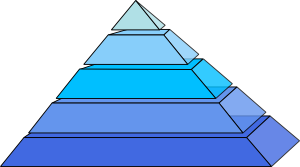
\includegraphics[width=1.1cm]{../Strukturfiler/FIGS/BluePyramid} & \begin{minipage}{\obsl}}{\end{minipage}\\ \end{tabular}\vspace{4mm}\newline}


% = Forudsætning = basis
\newenvironment{basis}{\begin{flushleft} \begin{itshape} }{\end{itshape} \end{flushleft}}


% = Opsummering =
\newenvironment{summary}{\clearpage\pagecolor{sumgul}\section{Opsummering}}{\newpage\pagecolor{white}}











% = Counter
\newcounter{opgavecount}[section]
\setcounter{opgavecount}{0}
\newcounter{spgcount}[opgavecount]
\setcounter{spgcount}{0}
\renewcommand{\thespgcount}{\alph{spgcount})}



% = EXERCISE = (DIVIDER)

\newcommand{\exercisebegin}[1][]{\bigskip\needspace{3\baselineskip}\refstepcounter{opgavecount}\titlegraphic{mingroen}\textcolor{mingroen}{\th{Opgave \theopgavecount \hspace*{1cm} #1}}\medskip\par}

% = QUIZEXERCISE = (DIVIDER)

\newcommand{\quizexercisebegin}[1][]{\bigskip\needspace{3\baselineskip}\refstepcounter{opgavecount}\titlegraphic{mingroen}\textcolor{mingroen}{\th{Quiz-Opgave \theopgavecount \hspace*{1cm} #1}}\medskip\par}

% = QUESTION =

\newenvironment{question}{\refstepcounter{spgcount}\begin{itemize}\item[\thespgcount]}{\end{itemize}\hspace*{\fill}}

% = VINK =

\newenvironment{vink}{\begin{tabular}{m{.9cm}<{\hspace*{2mm}}@{}|m{\obsl}@{}}\hspace*{-4pt}\raggedleft
\includegraphics[width=.9cm]{../Strukturfiler/FIGS/Think} & \begin{minipage}{\obsl}}{\end{minipage}\\ \end{tabular}\medskip\\}
	
% = FACIT =

\newenvironment{facit}{\begin{tabular}{m{.9cm}<{\hspace*{2mm}}@{}|m{\obsl}@{}}\hspace*{-4pt}\raggedleft
\includegraphics[width=.9cm]{../Strukturfiler/FIGS/Check} & \begin{minipage}{\obsl}}{\end{minipage}\\ \end{tabular}\medskip\\}








\newcommand{\afsnit}[1]{\bigskip\th{\titlegraphic{mingroen}\textcolor{mingroen}{#1}} \\ \rule[7pt]{.4\textwidth}{1pt} \vspace*{-2.5mm}\par}

% (DIVIDER):
\newcommand{\ugedagdatotitel}[4]{\pagebreak[4]\section{Semesteruge #1 -- #2 Dag \hspace*{1mm} (#3)} \vspace*{-4mm} \rule[5pt]{\textwidth}{1pt}\vspace*{-2.5mm} \begin{center}\large{\th{#4}}\end{center} \fancyhead[C]{\th{Semesteruge #1}}}

\newenvironment{skema}[1]{\definecolor{shadecolor}{rgb}{0.96,.98, 1.0} \setlength{\FrameSep}{6pt} \renewcommand{\FrameHeightAdjust}{10pt} \vspace*{-4pt}\begin{shaded} \begin{tabular}{#1}}{\end{tabular} \end{shaded} \vspace*{-7pt}}


% ========================

% MAKROER

%\newenvironment{matr}[1][]{\hspace*{-.8mm}\left[\hspace*{-1mm}\begin{array}{#1}}{\end{array}\hspace*{-1mm}\right]\hspace*{-.8mm}}
\newcommand{\bevisslut}{\begin{scriptsize} \begin{flushright} $ \blacksquare $ \end{flushright} \end{scriptsize}}

\newcommand{\tref}[2]{\hyperref[#1]{#2 \ref*{#1}}}
\newcommand{\thref}[2]{\hyperref[#1]{#2}}

\newcommand{\refA}[1]{\colorbox{yellow}{\ref{#1}}}
\newcommand{\hrefA}[2]{\colorbox{yellow}{\href{#1}{#2}}}
\newcommand{\trefA}[2]{\colorbox{yellow}{\hyperref[#1]{#2 \ref*{#1}}}}
\newcommand{\threfA}[2]{\colorbox{yellow}{\hyperref[#1]{#2}}}

\newenvironment{matr}[1]{\hspace*{-.8mm}\begin{bmatrix}\hspace*{-1mm}\begin{array}{#1}}{\end{array}\hspace*{-1mm}\end{bmatrix}\hspace*{-.8mm}}
\newcommand{\transp}{\hspace*{-.6mm}^{\top}}

\newcommand{\maengde}[2]{\left\lbrace \hspace*{-1mm} \begin{array}{c|c} #1 & #2 \end{array} \hspace*{-1mm} \right\rbrace}

\newenvironment{eqnalign}[1]{\setlength{\arraycolsep}{1.3pt}\begin{equation}\begin{array}{#1}}{\end{array}\end{equation}\par}
\newcommand{\eqnl}{\setlength{\arraycolsep}{1.3pt}}

\newcommand{\matind}[3]{{_\mathrm{#1}\mathbf{#2}_\mathrm{#3}}}
\newcommand{\vekind}[2]{{_\mathrm{#1}\mathbf{#2}}}
\newcommand{\jac}[2]{{\mathrm{Jacobi}_\mathbf{#1} (#2)}}
\newcommand{\diver}[2]{{\mathrm{div}\mathbf{#1} (#2)}}
\newcommand{\rot}[1]{{\mathbf{rot}\mathbf{(#1)}}}

\newcommand{\am}{\mathrm{am}}
\newcommand{\gm}{\mathrm{gm}}
\newcommand{\E}{\mathrm{E}}
\newcommand{\Span}{\mathrm{span}}
\newcommand{\mU}{\mathbf{U}}

\newcommand{\ms}{\medskip\\}
\newcommand{\bs}{\bigskip\\}

\newcommand{\mA}{\mathbf{A}}
\newcommand{\mB}{\mathbf{B}}
\newcommand{\mC}{\mathbf{C}}
\newcommand{\mD}{\mathbf{D}}
\newcommand{\mE}{\mathbf{E}}
\newcommand{\mF}{\mathbf{F}}
\newcommand{\mK}{\mathbf{K}}
\newcommand{\mI}{\mathbf{I}}
\newcommand{\mM}{\mathbf{M}}
\newcommand{\mN}{\mathbf{N}}
\newcommand{\mQ}{\mathbf{Q}}
\newcommand{\mT}{\mathbf{T}}
\newcommand{\mV}{\mathbf{V}}
\newcommand{\mW}{\mathbf{W}}
\newcommand{\mX}{\mathbf{X}}
\newcommand{\ma}{\mathbf{a}}
\newcommand{\mb}{\mathbf{b}}
\newcommand{\mc}{\mathbf{c}}
\newcommand{\md}{\mathbf{d}}
\newcommand{\me}{\mathbf{e}}
\newcommand{\mn}{\mathbf{n}}
\newcommand{\mr}{\mathbf{r}}
\newcommand{\mv}{\mathbf{v}}
\newcommand{\mw}{\mathbf{w}}
\newcommand{\mx}{\mathbf{x}}
\newcommand{\mxb}{\mathbf{x_{bet}}}
\newcommand{\my}{\mathbf{y}}
\newcommand{\mz}{\mathbf{z}}
\newcommand{\reel}{\mathbb{R}}
\newcommand{\mL}{\bm{\Lambda}} %Lambda-matrix
\newcommand{\mnul}{\bm{0}}
\newcommand{\trap}[1]{\mathrm{trap}(#1)}
\newcommand{\Det}{\operatorname{Det}}
\newcommand{\adj}{\operatorname{adj}}
\newcommand{\Ar}{\operatorname{Areal}}
\newcommand{\Vol}{\operatorname{Vol}}
\newcommand{\Rum}{\operatorname{Rum}}
\newcommand{\diag}{\operatorname{\bf{diag}}}
\newcommand{\bidiag}{\operatorname{\bf{bidiag}}}
\newcommand{\spanVec}[1]{\mathrm{span}\{#1\}}
\newcommand{\Div}{\operatorname{Div}}
\newcommand{\Rot}{\operatorname{\mathbf{Rot}}}

\newcommand{\Jac}{\operatorname{Jacobi}}
\newcommand{\Tan}{\operatorname{Tan}}
\newcommand{\Ort}{\operatorname{Ort}}
\newcommand{\Flux}{\operatorname{Flux}}
\newcommand{\Cmass}{\operatorname{Cm}}
\newcommand{\Imom}{\operatorname{Im}}
\newcommand{\Pmom}{\operatorname{Pm}}
\newcommand{\IS}{\operatorname{I}}
\newcommand{\IIS}{\operatorname{II}}
\newcommand{\IIIS}{\operatorname{III}}
\newcommand{\Le}{\operatorname{L}}
\newcommand{\app}{\operatorname{app}}
\newcommand{\M}{\operatorname{M}}
\newcommand{\re}{\mathrm{Re}}
\newcommand{\im}{\mathrm{Im}}

\newcommand{\compl}{\mathbb{C}} %de komplekse tal
\newcommand{\e}{\mathrm{e}} %eksponentialfunktionen. lodret 'e', og altså ikke kursiv ligesom andre bogstaver.





% Medialink: SCREEN: (QRcode) + thumbnail image + link på kodenummer (til qr.dtu.dk)
\newcommand{\onlinemedia}[3]{
	\begin{wrapfigure}{r}{3.2cm} 
		\vspace{-30pt} 
		\vspace{#1pt} 
		\begin{flushright} 
			\includegraphics[width=3cm]{qr/#2.png} 
			\tiny 
			\href{http://qr.dtu.dk/#2}{#2: #3}
			\normalsize  
		\end{flushright} 
		\vspace{-10pt} 
	\end{wrapfigure}
}
\newcommand{\onlinemediathumb}[3]{
	\begin{wrapfigure}{r}{3.2cm} 
		\vspace{-30pt} 
		\vspace{#1pt} 
		\begin{flushright} 
			\includegraphics[width=3cm]{qr/#2.png} 
			\includegraphics[width=3cm]{qr/#2_thumb.png} 
			\tiny 
			\href{http://qr.dtu.dk/#2}{#2: #3}
			\normalsize  
		\end{flushright} 
		\vspace{-10pt} 
	\end{wrapfigure}
}



% Index:
\usepackage{makeidx}
\makeindex
\newcommand\ind[2]{\index{#1}\textbf{\textit{\textcolor{black}{#2}}}}

% ###SERVER_EXCLUDE_BEGIN###
\externaldocument[NUID17-]{../../enoten/TN01-Talrum/Talrum}
\externaldocument[NUID1-]{../../enoten/TN02-Ligningssystemer/TNdriver}
\externaldocument[NUID2-]{../../enoten/TN03-Matricer_og_Matrixalgebra/Matricer_og_matrixalgebra}
\externaldocument[NUID3-]{../../enoten/TN04-Kvadratiske_matricer/TNdriver}
\externaldocument[NUID11-]{../../enoten/TN05-Determinanter/Determinanter}
\externaldocument[NUID12-]{../../enoten/TN06-GeometriskeVektorer/GeometriskeVektorer}
\externaldocument[NUID18-]{../../enoten/TN07-Vektorrum/VektorRum}
\externaldocument[NUID21-]{../../enoten/TN08-LinAfbildninger/LinAfbildninger}
\externaldocument[NUID23-]{../../enoten/TN09-Egenvaerdier_og_egenvektorer/TNdriver}
\externaldocument[NUID24-]{../../enoten/TN10-Diagonalisering_med_egenvektorer/TNdriver}
\externaldocument[NUID10-]{../../enoten/TN11-1.ordens_differentialligninger/TNdriver}
\externaldocument[NUID13-]{../../enoten/TN12-1.ordens_differentialligningssystemer/TNdriver}
\externaldocument[NUID14-]{../../enoten/TN13-2.ordens_differentialligninger/TNdriver}
\externaldocument[NUID27-]{../../enoten/TN14-Elemenataere_funktioner/Elementaere_Funktioner}
\externaldocument[NUID28-]{../../enoten/TN15-Funktioner2Variable/Funktioner_To_Variable}
\externaldocument[NUID29-]{../../enoten/TN16-Gradienter_og_Tangentplaner/Gradienter_og_Tangentplaner}
\externaldocument[NUID32-]{../../enoten/TN17-Taylor_formler/Taylor_Formler}
\externaldocument[NUID33-]{../../enoten/TN18-Taylor_2Var/Taylor_2Var}
\externaldocument[NUID34-]{../../enoten/TN19-SymMat/SymmetriskeMatricer}
\externaldocument[NUID35-]{../../enoten/TN20-KegleSnit/Keglesnit}
\externaldocument[NUID36-]{../../enoten/TN21-Riemann_Integral/Riemann_01}
\externaldocument[NUID37-]{../../enoten/TN22-Plan_Int/Plan_Int_01}
\externaldocument[NUID39-]{../../enoten/TN23-Flade_Int/Flade_Rum_Int_01}
\externaldocument[NUID40-]{../../enoten/TN24-Vektorfelter/Vektorfelter_01}
\externaldocument[NUID41-]{../../enoten/TN25-Flux/Flux_02}
\externaldocument[NUID42-]{../../enoten/TN26-Gauss/Gauss_01}
\externaldocument[NUID128-]{../../enoten/TN27-Stokes/Stokes_01}
\externaldocument[NUID43-]{../../enoten/TN29-KomplekseTal/KomplekseTal}

\externaldocument[NUID6-]{../../E-math-opgaver/Opgaver/opgU123}
\externaldocument[NUID19-]{../../E-math-opgaver/Opgaver/opgU45}
\externaldocument[NUID20-]{../../E-math-opgaver/Opgaver/opgU678}
\externaldocument[NUID25-]{../../E-math-opgaver/Opgaver/opgU910SD}
\externaldocument[NUID31-]{../../E-math-opgaver/OpgaverF11-U123/opgF123}
% \externaldocument[NUID9-]{../../E-math-opgaver/Opgaver/Dagsordner E10}
% ###SERVER_EXCLUDE_END###


% Begin document and set alternative chapter title:
\begin{document}
\renewcommand{\chaptername}{eNote}

\setcounter{chapter}{23} %SÆT DETTE TAL TIL 1 MINDRE END DET AKTUELLE TRANSFERNOTE-NUMMER!!

%%%%%%%%%%%%%%%%%%%%%%%%%%%%%%%%%%%%%%%%%%%%%
%%%%%%%%%%%%%%%%%%%%%%%%%%%%%%%%%%%%%%%%%%%%%
%%% HERFRA SKAL DU SKadsfRIVE ELLER INDSÆTTE %%%%
%%% DEN FIL DU ØNSKER %%%%%%%%%%%%%%%%%%%%%%%
%%%%%%%%%%%%%%%%%%%%%%%%%%%%%%%%%%%%%%%%%%%%%
%%%%%%%%%%%%%%%%%%%%%%%%%%%%%%%%%%%%%%%%%%%%%


% REF: TransferNote \ref{TN4-tn4} \nameref{TN4-tn4}
%
% \tref{NUID14-thm.koma}{sætning} \tref{NUID28-tn15}{eNote}
%
%\tref{NUID34-tn19}{eNote} Symmetriske matricer
%\tref{NUID33-tn18}{eNote} Taylor i 2 variable
%
% 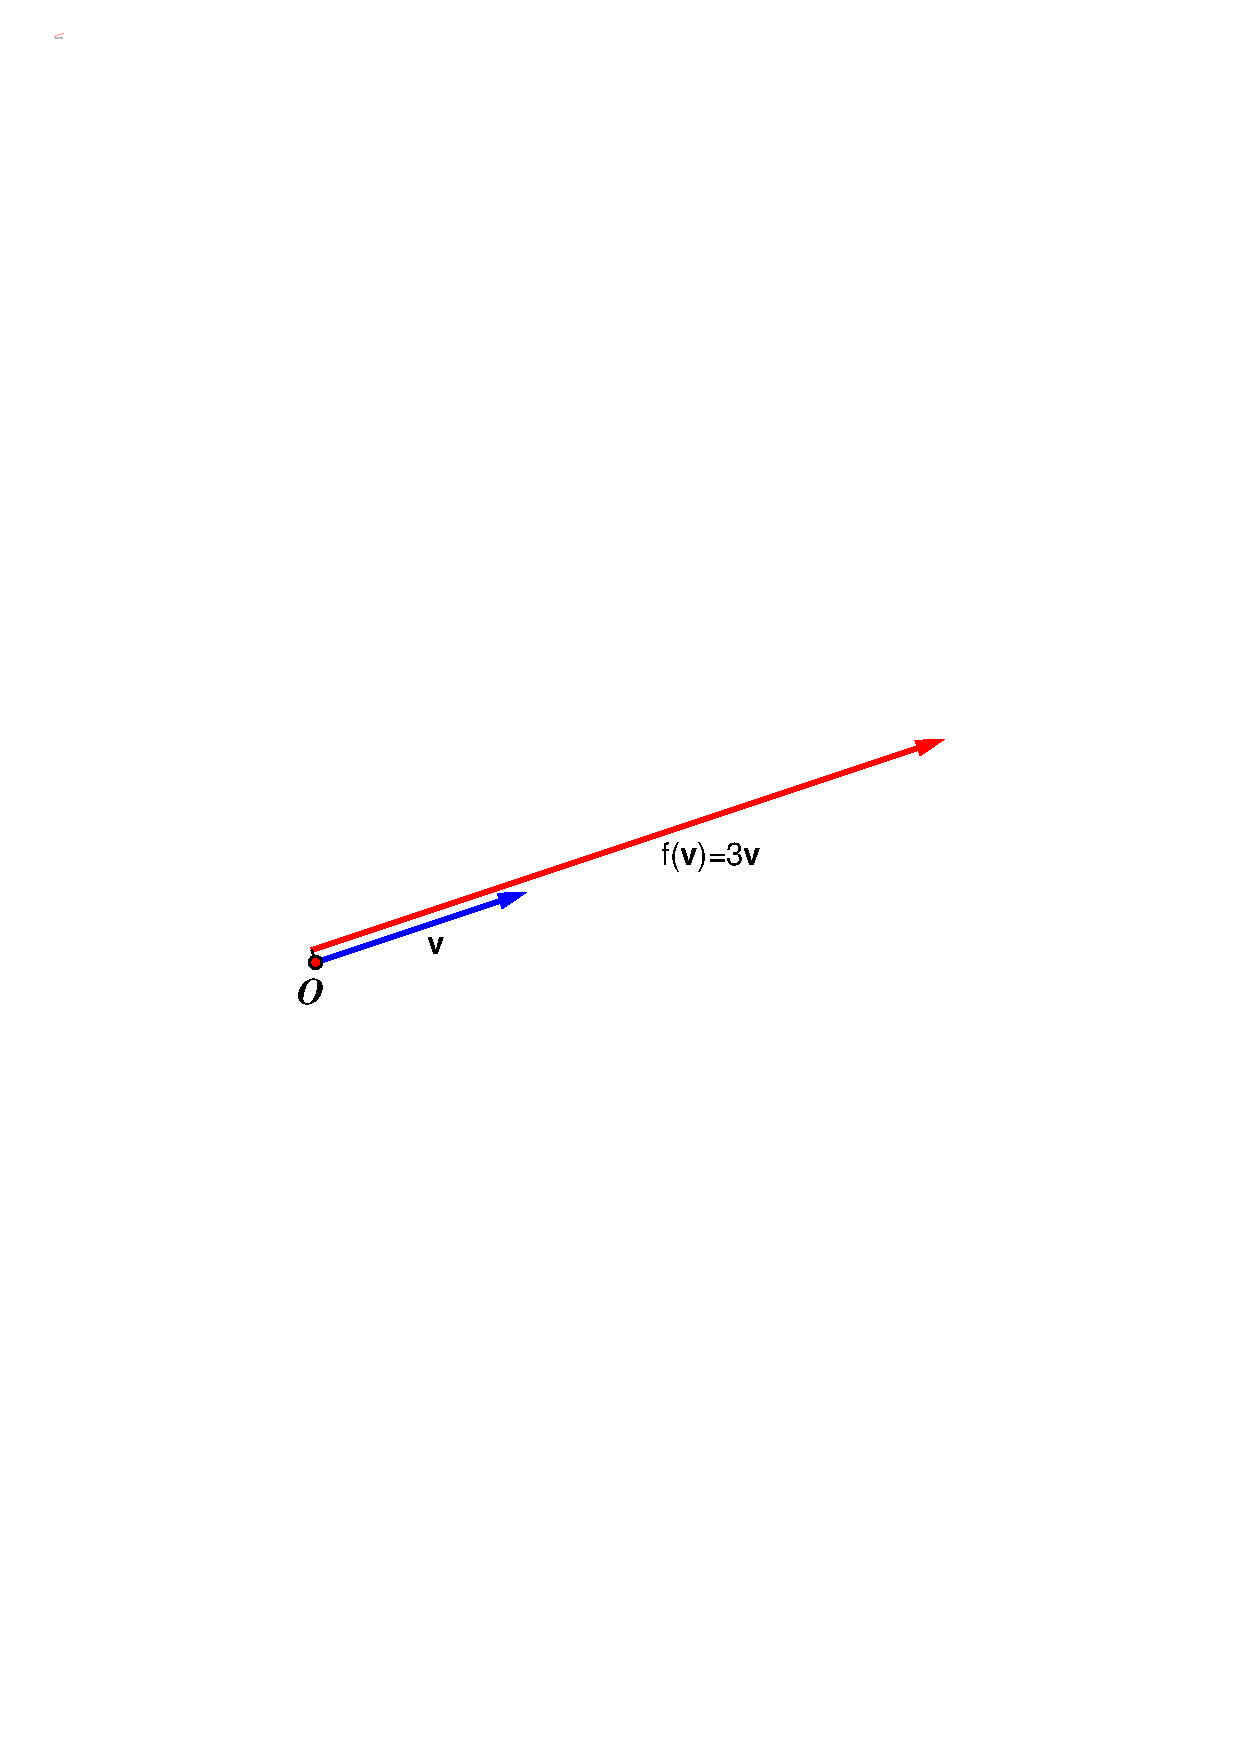
\includegraphics[trim=5cm 12cm 5cm 12cm,width=0.40\textwidth,clip]{skalering.pdf}
%
%\begin{equation}
%\matind vMa \cdot \matind aFa \cdot \matind aMv = \matind vFv \, ,
%\end{equation}
%hvor
%\begin{equation}
%\matind aMv = \begin{matr}{cccc} \vekind av_1 & \vekind av_2 & \cdots & \vekind av_n \end{matr} \quad \mathrm{og} \quad %\matind vFv = \diag(\lambda_1, \lambda_2, \ldots, \lambda_n) \, .
%\end{equation}
%
%$\vekind{e}{F}$
%$\matind{e}{F}{w}$
%
%\href{http://www-groups.dcs.st-and.ac.uk/~history/}{http://www-groups.dcs.st-and.ac.uk/~history/}

%%%%%%%%%%%%%%%%%%%%%%%%%%%%%%%%%%%%%%%%%%%%%%%%%%%
%%%%%%%%%%%%%%%%%%%%%%%%%%%%%%%%%%%%%%%%%%%%%%%%%%%
%%%%%%%%%%%%%%%%%%%%%%%%%%%%%%%%%%%%%%%%%%%%%%%%%%%
%%%%%%%%%%%%%%%%%%%%%%%%%%%%%%%%%%%%%%%%%%%%%%%%%%%

\chapter{Vektorfelter} \label{tn24}


\begin{basis}
I \tref{NUID12-tn6}{eNote}  indføres og studeres vektorer i plan og rum. I \tref{NUID29-tn16}{eNote} ser vi på gradienterne for funktioner $f(x,y)$ af to variable. Et gradientvektorfelt for en funktion af to variable er -- som navnet rigeligt antyder -- et eksempel på et plant vektorfelt. I denne eNote vil vi begynde at studere vektorfelter helt generelt. Både i planen og i rummet. Vi vil præcisere, hvad det betyder at \emph{flyde med et givet vektorfelt} og beregne, hvor man kommer hen i rummet  eller i planen på den måde i løbet af et givet tidsrum. For at finde disse såkaldte \emph{flow-kurver} får vi  brug for at kunne løse (her passende simple) første ordens differentialligningssystemer hvorved \tref{NUID13-tn12}{eNote} ligesom de ovenfor nævnte eNoter bliver aktuelt materiale for nærværende eNote. Vi vil også begynde på at undersøge, hvad der sker med større systemer af punkter eller partikler når de hver for sig flyder med vektorfeltet.
\end{basis}



%%%%%%%%%%%%%%%%%%%%%%%%%%%%%%%%%%%%%%%%%%%%%%%%%%%
%%%%%%%%%%%%%%%%%%%%%%%%%%%%%%%%%%%%%%%%%%%%%%%%%%%
%%%%%%%%%%%%%%%%%%%%%%%%%%%%%%%%%%%%%%%%%%%%%%%%%%%
%%%%%%%%%%%%%%%%%%%%%%%%%%%%%%%%%%%%%%%%%%%%%%%%%%%






\section{Vektorfelter} \label{secVektorfelter}

Et {vektorfelt} $\mathbf{V}$ i \emph{rummet} er givet ved $3$ glatte funktioner
$V_{1}(x,y,z)\,$, $V_{2}(x,y,z)\,$ og  $V_{3}(x,y,z)\,$ som hver er funktioner af de tre variable $x$, $y$, og $z$ således:
\begin{equation}
{\mathbf{V}}(x,y,z) = \left(V_{1}(x,y,z)\,, V_{2}(x,y,z)\,,
V_{3}(x,y,z)\,\right) \quad {\text{for}}\quad (x,y,z) \in
\mathbb{R}^{3} \quad .
\end{equation}

\begin{info}
Et vektorfelt $\mathbf{V}(x,y,z)$ \emph{tegnes} og angives sædvanligvis i rummet ved i et passende antal udvalgte punkter $(x_{i}, y_{i}, z_{i})$ at afsætte vektoren som en pil med fodpunkt i  $(x_{i}, y_{i}, z_{i})$ og spidspunkt i $(x_{i}+ V_{1}(x_{i}, y_{i}, z_{i}), y_{i}+V_{2}(x_{i}, y_{i}, z_{i}), z_{i}+ V_{3}(x_{i}, y_{i}, z_{i}))$. Der kan være gode grunde til at angive vektorfeltet på andre måder. F.eks. hvis der er stor variation i længden af vektorerne i et givet område, så kan det være en fordel at benytte \emph{tykkelsen} af pilene som en længde-indikerende parameter.
\end{info}

Et vektorfelt i planen er tilsvarende givet ved to koordinatfunktioner $V_{1}(x,y)\,$ og $V_{2}(x,y)\,$ som hver er glatte funktioner af de to variable $x$ og $y$:
\begin{equation}
{\mathbf{V}}(x,y) = \left(V_{1}(x,y)\,, V_{2}(x,y)\,\right) \quad {\text{for}}\quad (x,y) \in
\mathbb{R}^{2} \quad .
\end{equation}

Gradientvektorfeltet for en glat funktion $f(x,y)$  af to variable (som indføres og studeres i \tref{NUID29-tn16}{eNote})  er et eksempel på et vektorfelt i planen, se figur \ref{figGradFelt}. \\

\begin{figure}[h]
\centerline{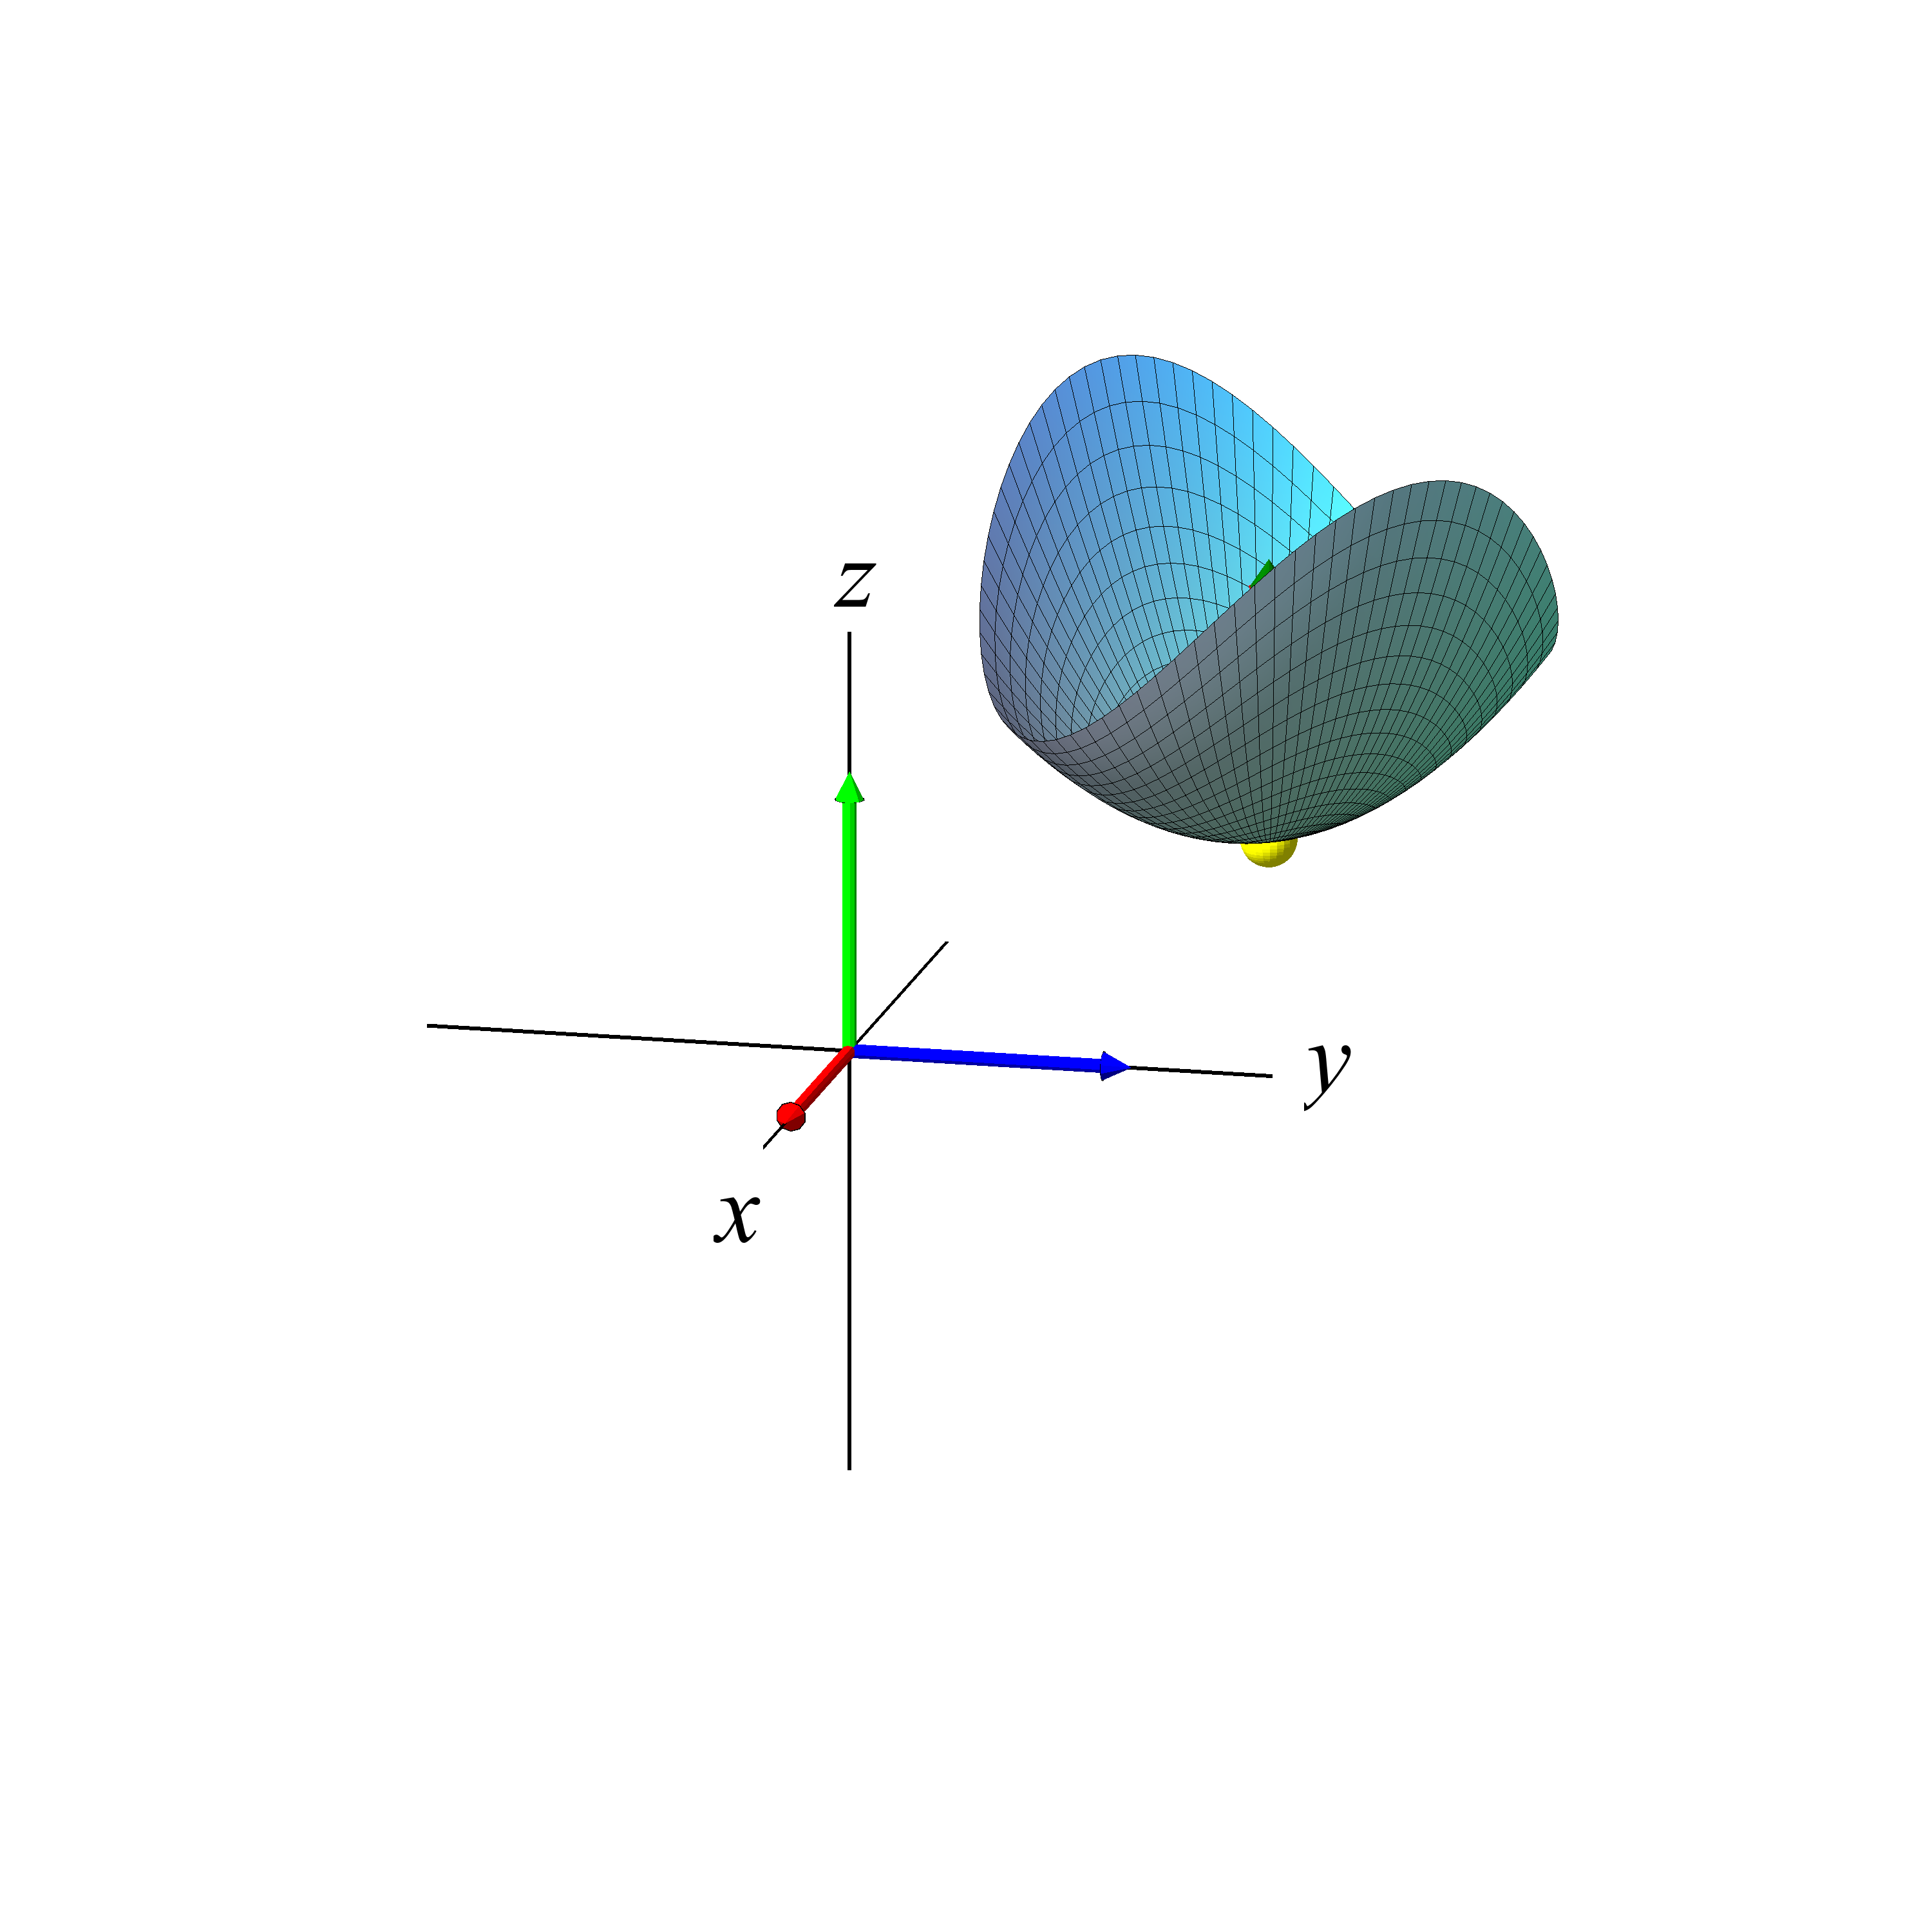
\includegraphics[height=90mm]{FIGS/plotVar2Fig4}\,\,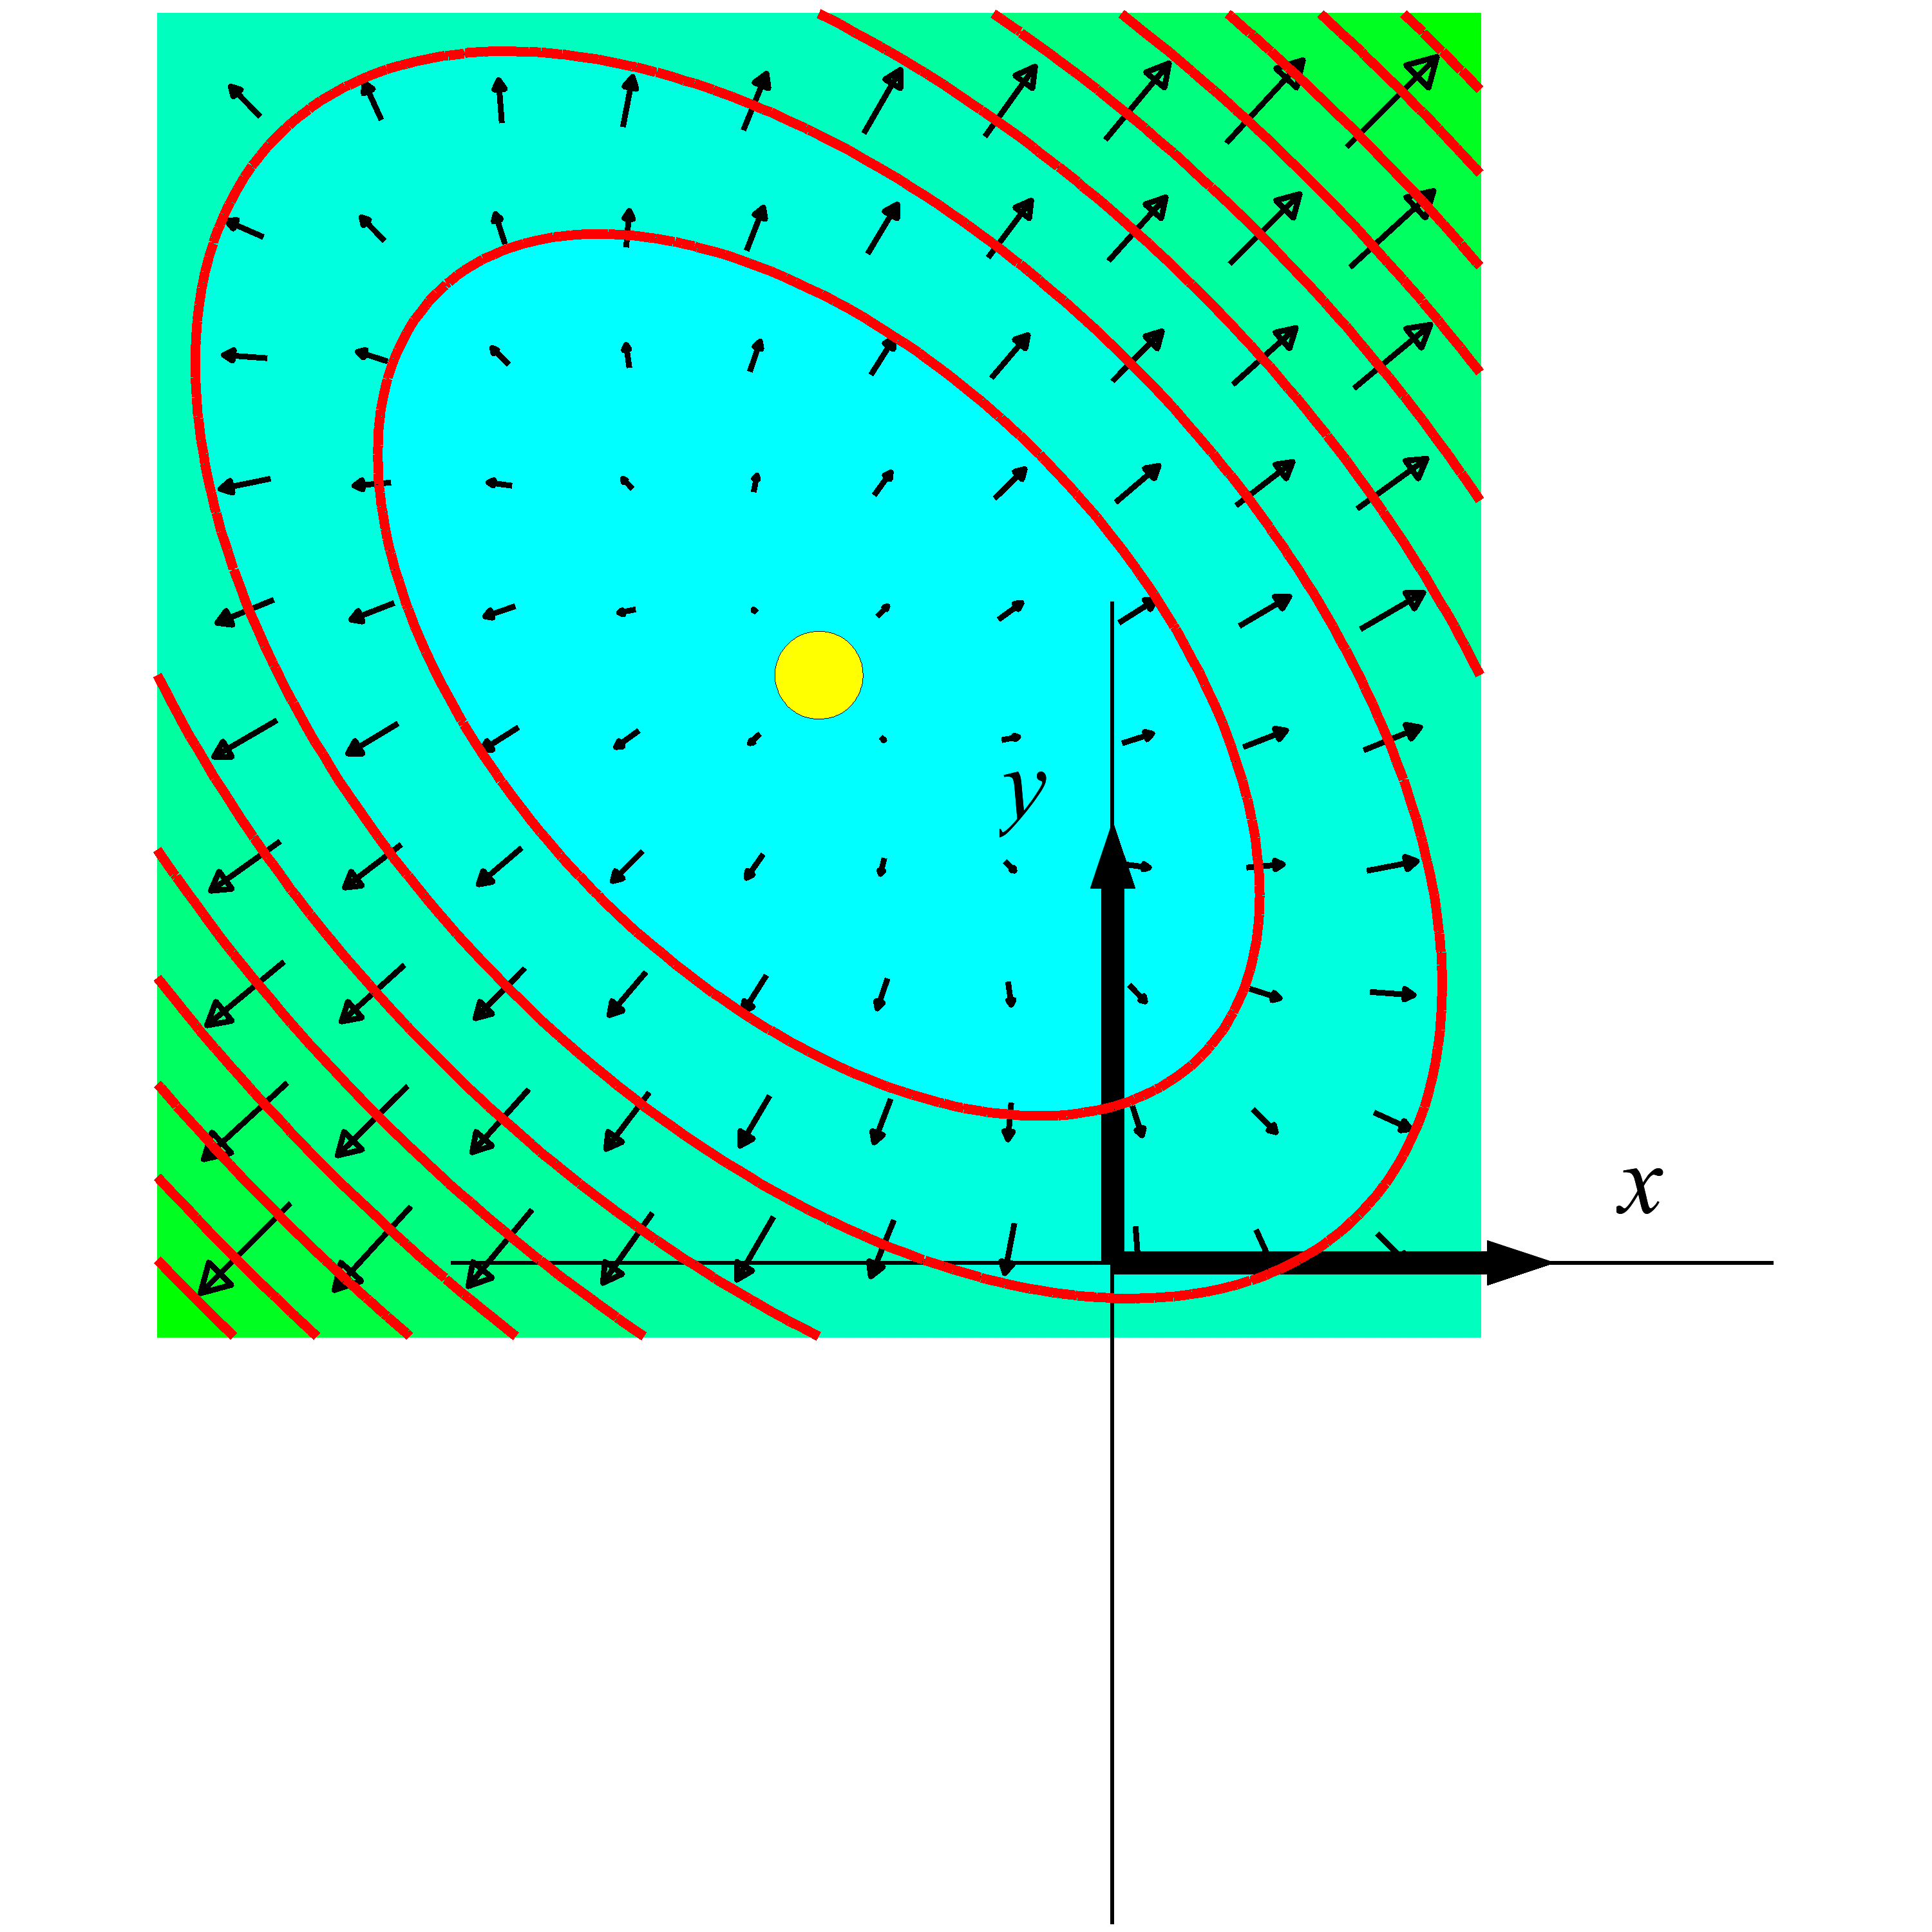
\includegraphics[height=90mm]{FIGS/plotGrad4}}
\begin{center}
\caption{\small{En grafflade for en funktion af to variable og det tilhørende gradientvektorfelt i planen sammen med nogle af niveaukurverne. Gradientvektorfeltet er overalt vinkelret på niveaukurverne, se \tref{NUID29-tn16}{eNote}.}}
\label{figGradFelt}
\end{center}
\end{figure}

Som for funktioner af tre variable defineres gradientvektorfeltet for funktioner $f(x,y, z)$  af tre variable:


\begin{definition}[Gradientfelt i rummet] \label{defGradFelt3D}
Lad $f(x,y,z)$ betegne en glat funktion af tre variable i $\mathbb{R}^{3}$.
Så defineres gradientvektorfeltet for $f(x,y,z)$ på følgende måde ved hjælp af de tre første partielle afledede af $f(x,y,z)$:
\begin{equation}
\bm{\nabla}f(x,y,z) = \left(f'_{x}(x,y,z)\, , \, f'_{y}(x,y,z) \, , \, f'_{z}(x,y,z)\right) \quad , \quad (x,y,z) \in \mathbb{R}^{3} \quad .
\end{equation}
\end{definition}

\begin{example}[Et gradientfelt i rummet] \label{exampGradFelter}
Vi lader $f(x,y,z)$ betegne andengradspolynomiet
\begin{equation}
f(x,y, z) =  2\cdot x^{2} + 2\cdot y^{2} + 2\cdot z^{2} - 2\cdot x \cdot z - 2\cdot x - 4\cdot y - 2 \cdot z +3 \quad .
\end{equation}
Gradientvektorfeltet for $f(x,y,z)$ er så:
\begin{equation}
\bm{\nabla}f(x,y,z) = ( 4\cdot x - 2\cdot z -2\, , \, 4\cdot y - 4 \, , \, -2\cdot x + 4 \cdot z - 2  ) \quad .
\end{equation}
Se  figur \ref{figGradFelt3D}. Vi refererer til \tref{NUID35-exampEllipsoide}{eksempel} i  \tref{NUID35-tn20}{eNote} vedrørende konstruktionen af den viste ellipsoide-niveauflade $\mathcal{K}_{0}(f)$ for $f(x,y,z)$. Niveaufladen og det beregnede gradientvektorfelt er antydet i figur \ref{figGradFelt3D}. Gradientvektorfeltet ses at være vinkelret på niveaufladen.
\end{example}


\begin{figure}[ht]
\centerline{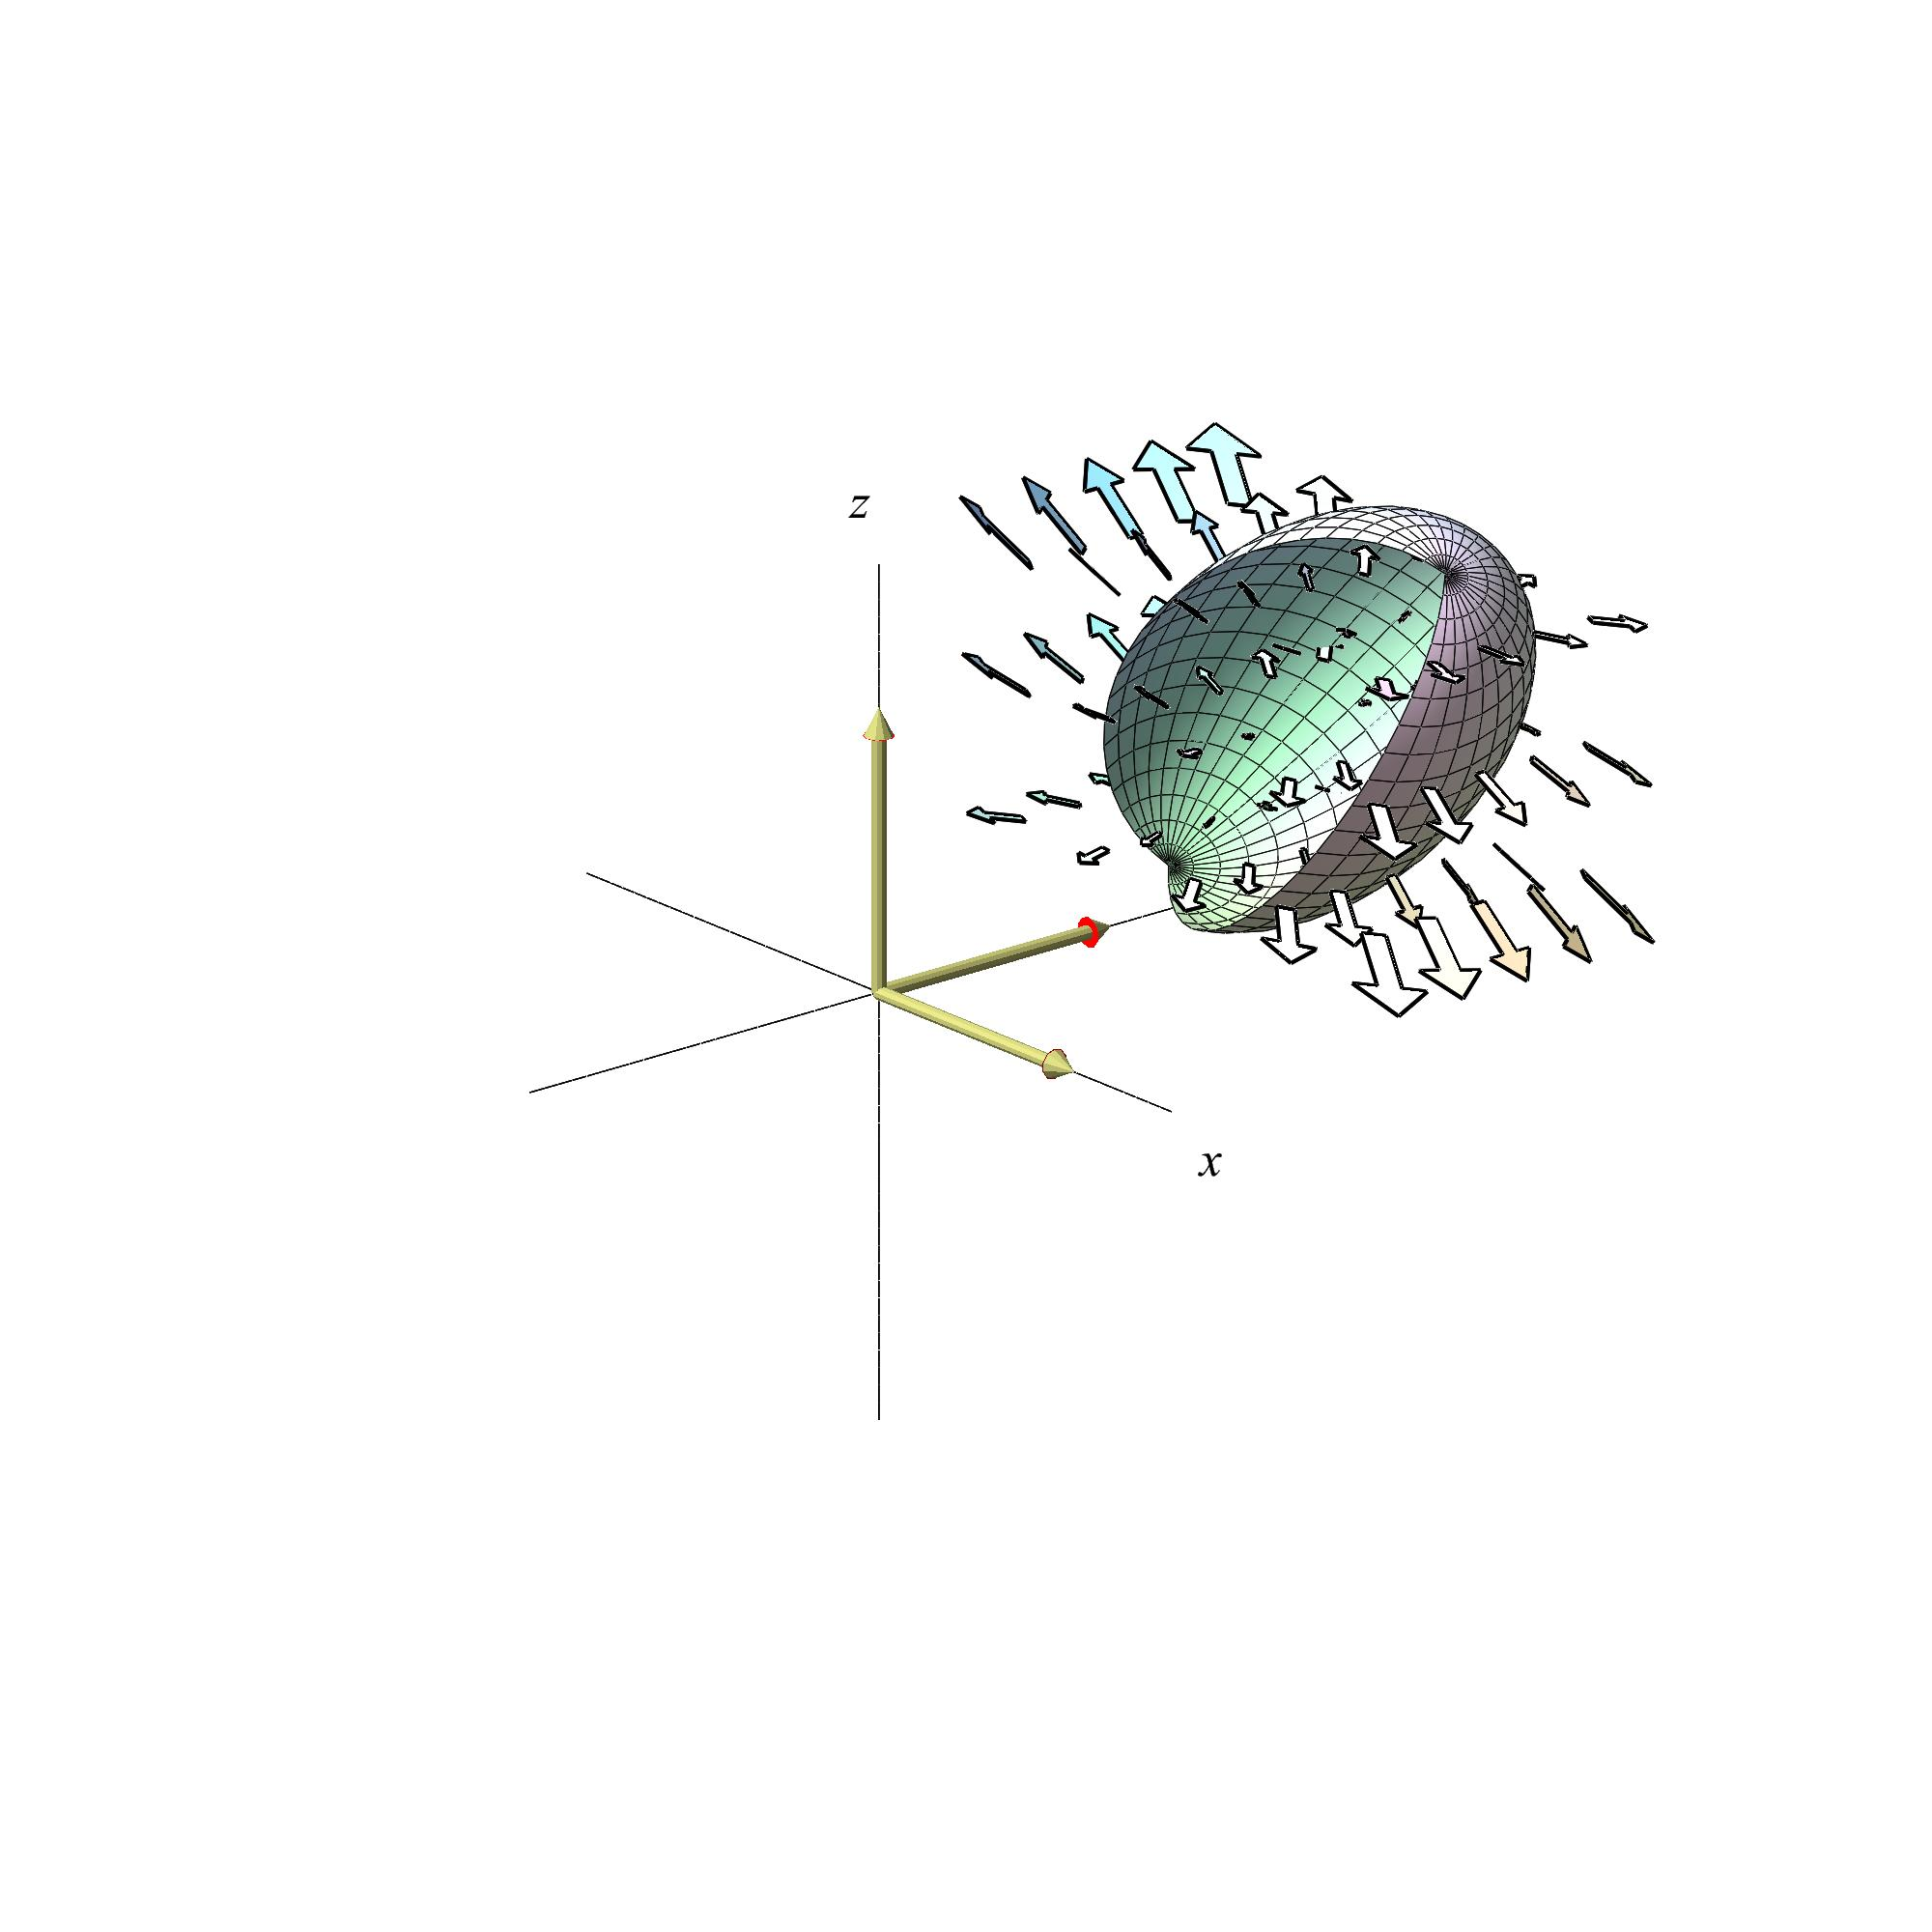
\includegraphics[height=90mm]{FIGS/plotGradFeltEllip2}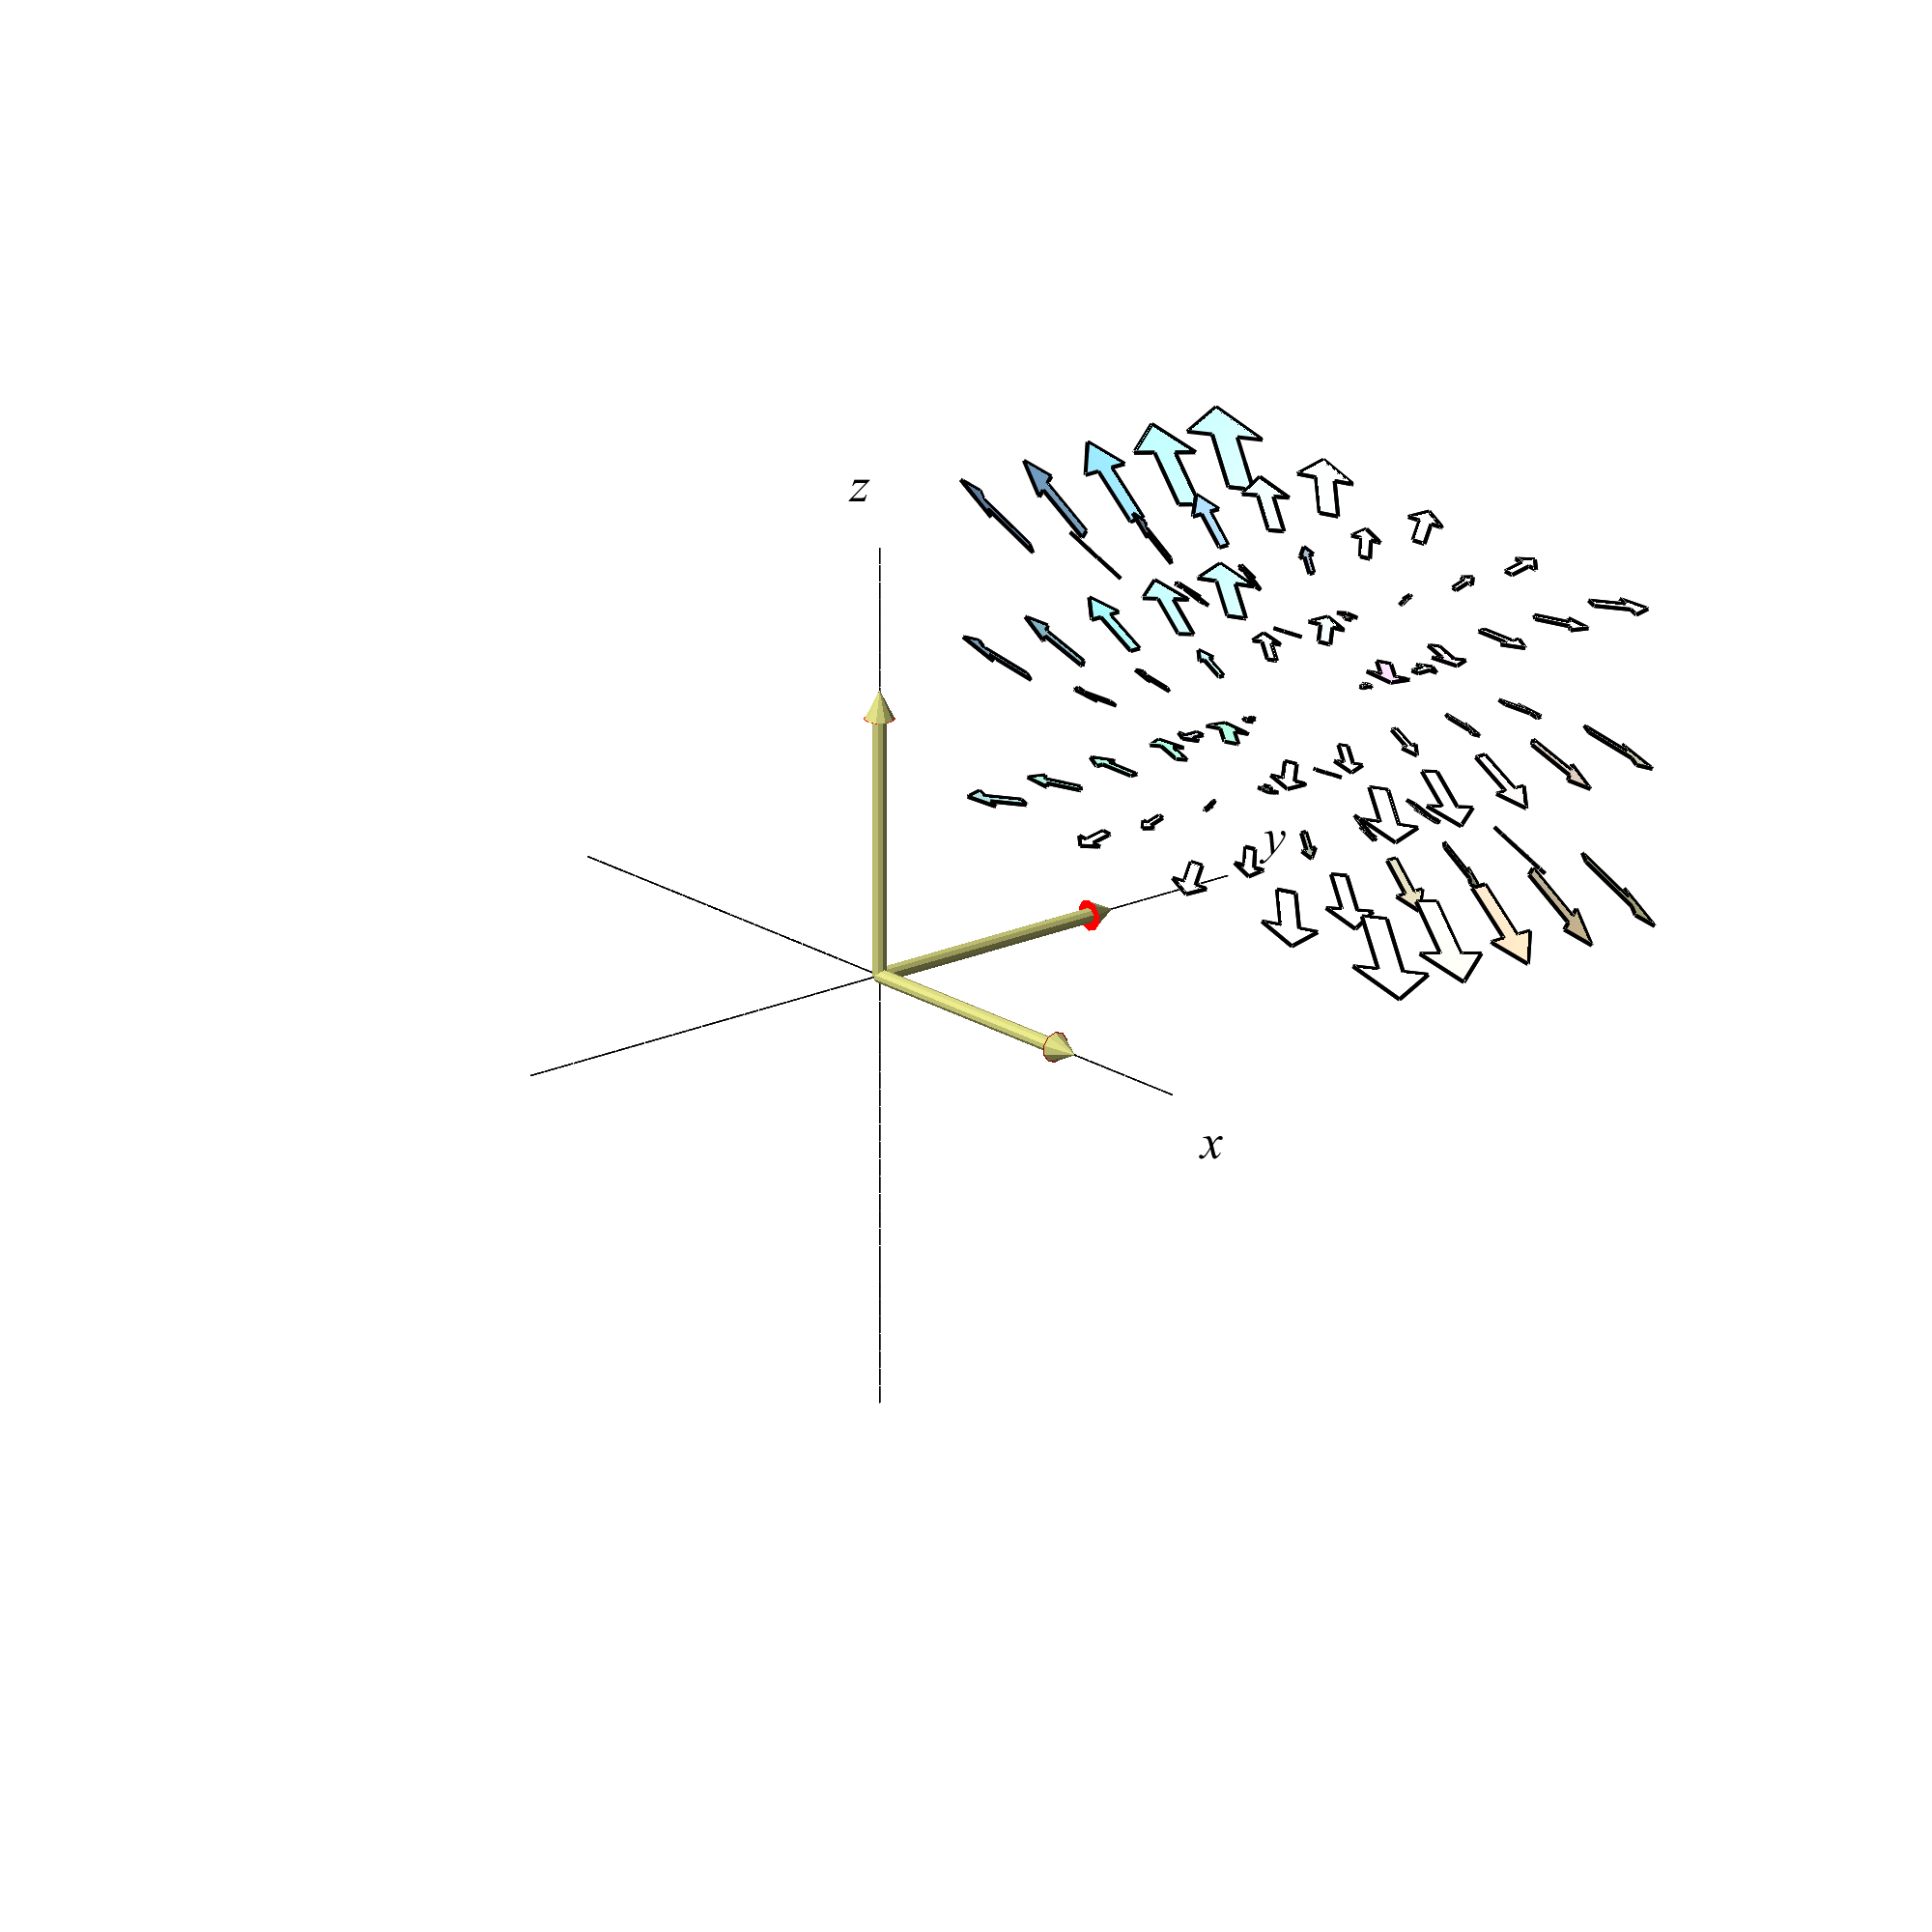
\includegraphics[height=90mm]{FIGS/plotGradFeltEllip1}}
\begin{center}
\caption{\small{Niveauflade (i åbnet version) for en funktion (andengradspolynomium) af tre variable og nogle tilhørende gradientvektorer fra gradientvektorfeltet i rummet.}}
\label{figGradFelt3D}
\end{center}
\end{figure}



\begin{aha}
Man kan nu meget vel spørge om \emph{alle} glatte vektorfelter i planen og \emph{alle} glatte vektorfelter i rummet
\emph{stammer fra} en funktion på den måde, at de hver for sig er gradientvektorfeltet for en eller anden funktion af henholdsvis to og tre variable. Men så simpelt er det ikke!
\end{aha}


\begin{example}[Et vektorfelt som ikke er et gradientvektorfelt] \label{exampNonGradFelt}
Lad $\mathbf{V}(x,y)$ betegne det meget simple vektorfelt i planen $\mathbf{V}(x,y) = (-y, x)$, hvor $(x,y)\in \mathbb{R}^{2}$. Så findes der ikke nogen funktion $f(x,y)$ som opfylder at $\bm{\nabla}f(x,y) = \mathbf{V}(x,y)$. \\

Hvis vi nemlig (indtil modstrid) antager, at der findes en sådan funktion med den egenskab:
\begin{equation}
\begin{aligned}
\bm{\nabla}f(x,y) &= \mathbf{V}(x,y) \quad , \quad \textrm{sådan at} \\
\left(f'_{x}(x,y), f'_{y}(x,y) \right) &= (-y, x) \quad , \quad \textrm{så får vi at} \\ \\
f'_{x}(x,y) &= -y \\
f'_{y}(x,y) &= x \quad , \quad \textrm{og dermed} \\ \\
f''_{x y}(x,y) &= -1 \\
f''_{y x}(x,y) &= 1 \quad ,
\end{aligned}
\end{equation}
og det stemmer jo ikke overens med at der for alle glatte funktioner gælder
\begin{equation}
f''_{x y}(x,y) = f''_{yx}(x,y) \quad , \quad \textrm{for alle} \quad (x,y) \in \mathbb{R}^{2} \quad .
\end{equation}
Det viser, at der ikke findes nogen funktion hvis gradientvektorfelt er det givne vektorfelt.
\end{example}

\begin{think}
Gradientvektorfelterne er altså kun eksempler på vektorfelter -- men en meget stor og meget vigtig samling af eksempler på vektorfelter.
\end{think}

\begin{aha}
Et vektorfelt $\mathbf{V}(x,y)$ i planen kan let udvides til et vektorfelt $\mathbf{W}(x,y,z)$ i rummet ved simpelthen at parallelforskyde alle vektorerne fra planen i  $z$-aksens retning og iøvrigt sætte
$W_{3}(x,y,z) = 0$ for alle $(x,y,z) \in \mathbb{R}^{3}$: \\

Det helt generelle plane vektorfelt $\mathbf{V}(x,y) = (V_{1}(x,y), V_{2}(x,y))$ har således følgende rumlige udvidelse:
\begin{equation}
\begin{aligned}
\mathbf{W}(x,y,z) &= (V_{1}(x,y), V_{2}(x,y), 0) \quad \textrm{dvs.} \\ \\
W_{1}(x,y,z) &= V_{1}(x,y) \quad ,\\
W_{2}(x,y,z) &= V_{2}(x,y) \quad ,\\
W_{3}(x,y,z) &= 0 \quad .
\end{aligned}
\end{equation}
Se figur \ref{figVFUdvidet} som antyder de rumlige udvidelser af tre forskellige  vektorfelter $\mathbf{V}(x,y) = (1,0)$, $\mathbf{V}(x,y) = (x,y)$, og $\mathbf{V}(x,y) = (-y, x)$,  altså $\mathbf{W}(x,y,z) = (1,0,0)$, $\mathbf{W}(x,y,z) = (x,y,0)$, og $\mathbf{W}(x,y,z) = (-y, x, 0)$ henholdsvis.
\end{aha}

\begin{figure}[ht]
\centerline{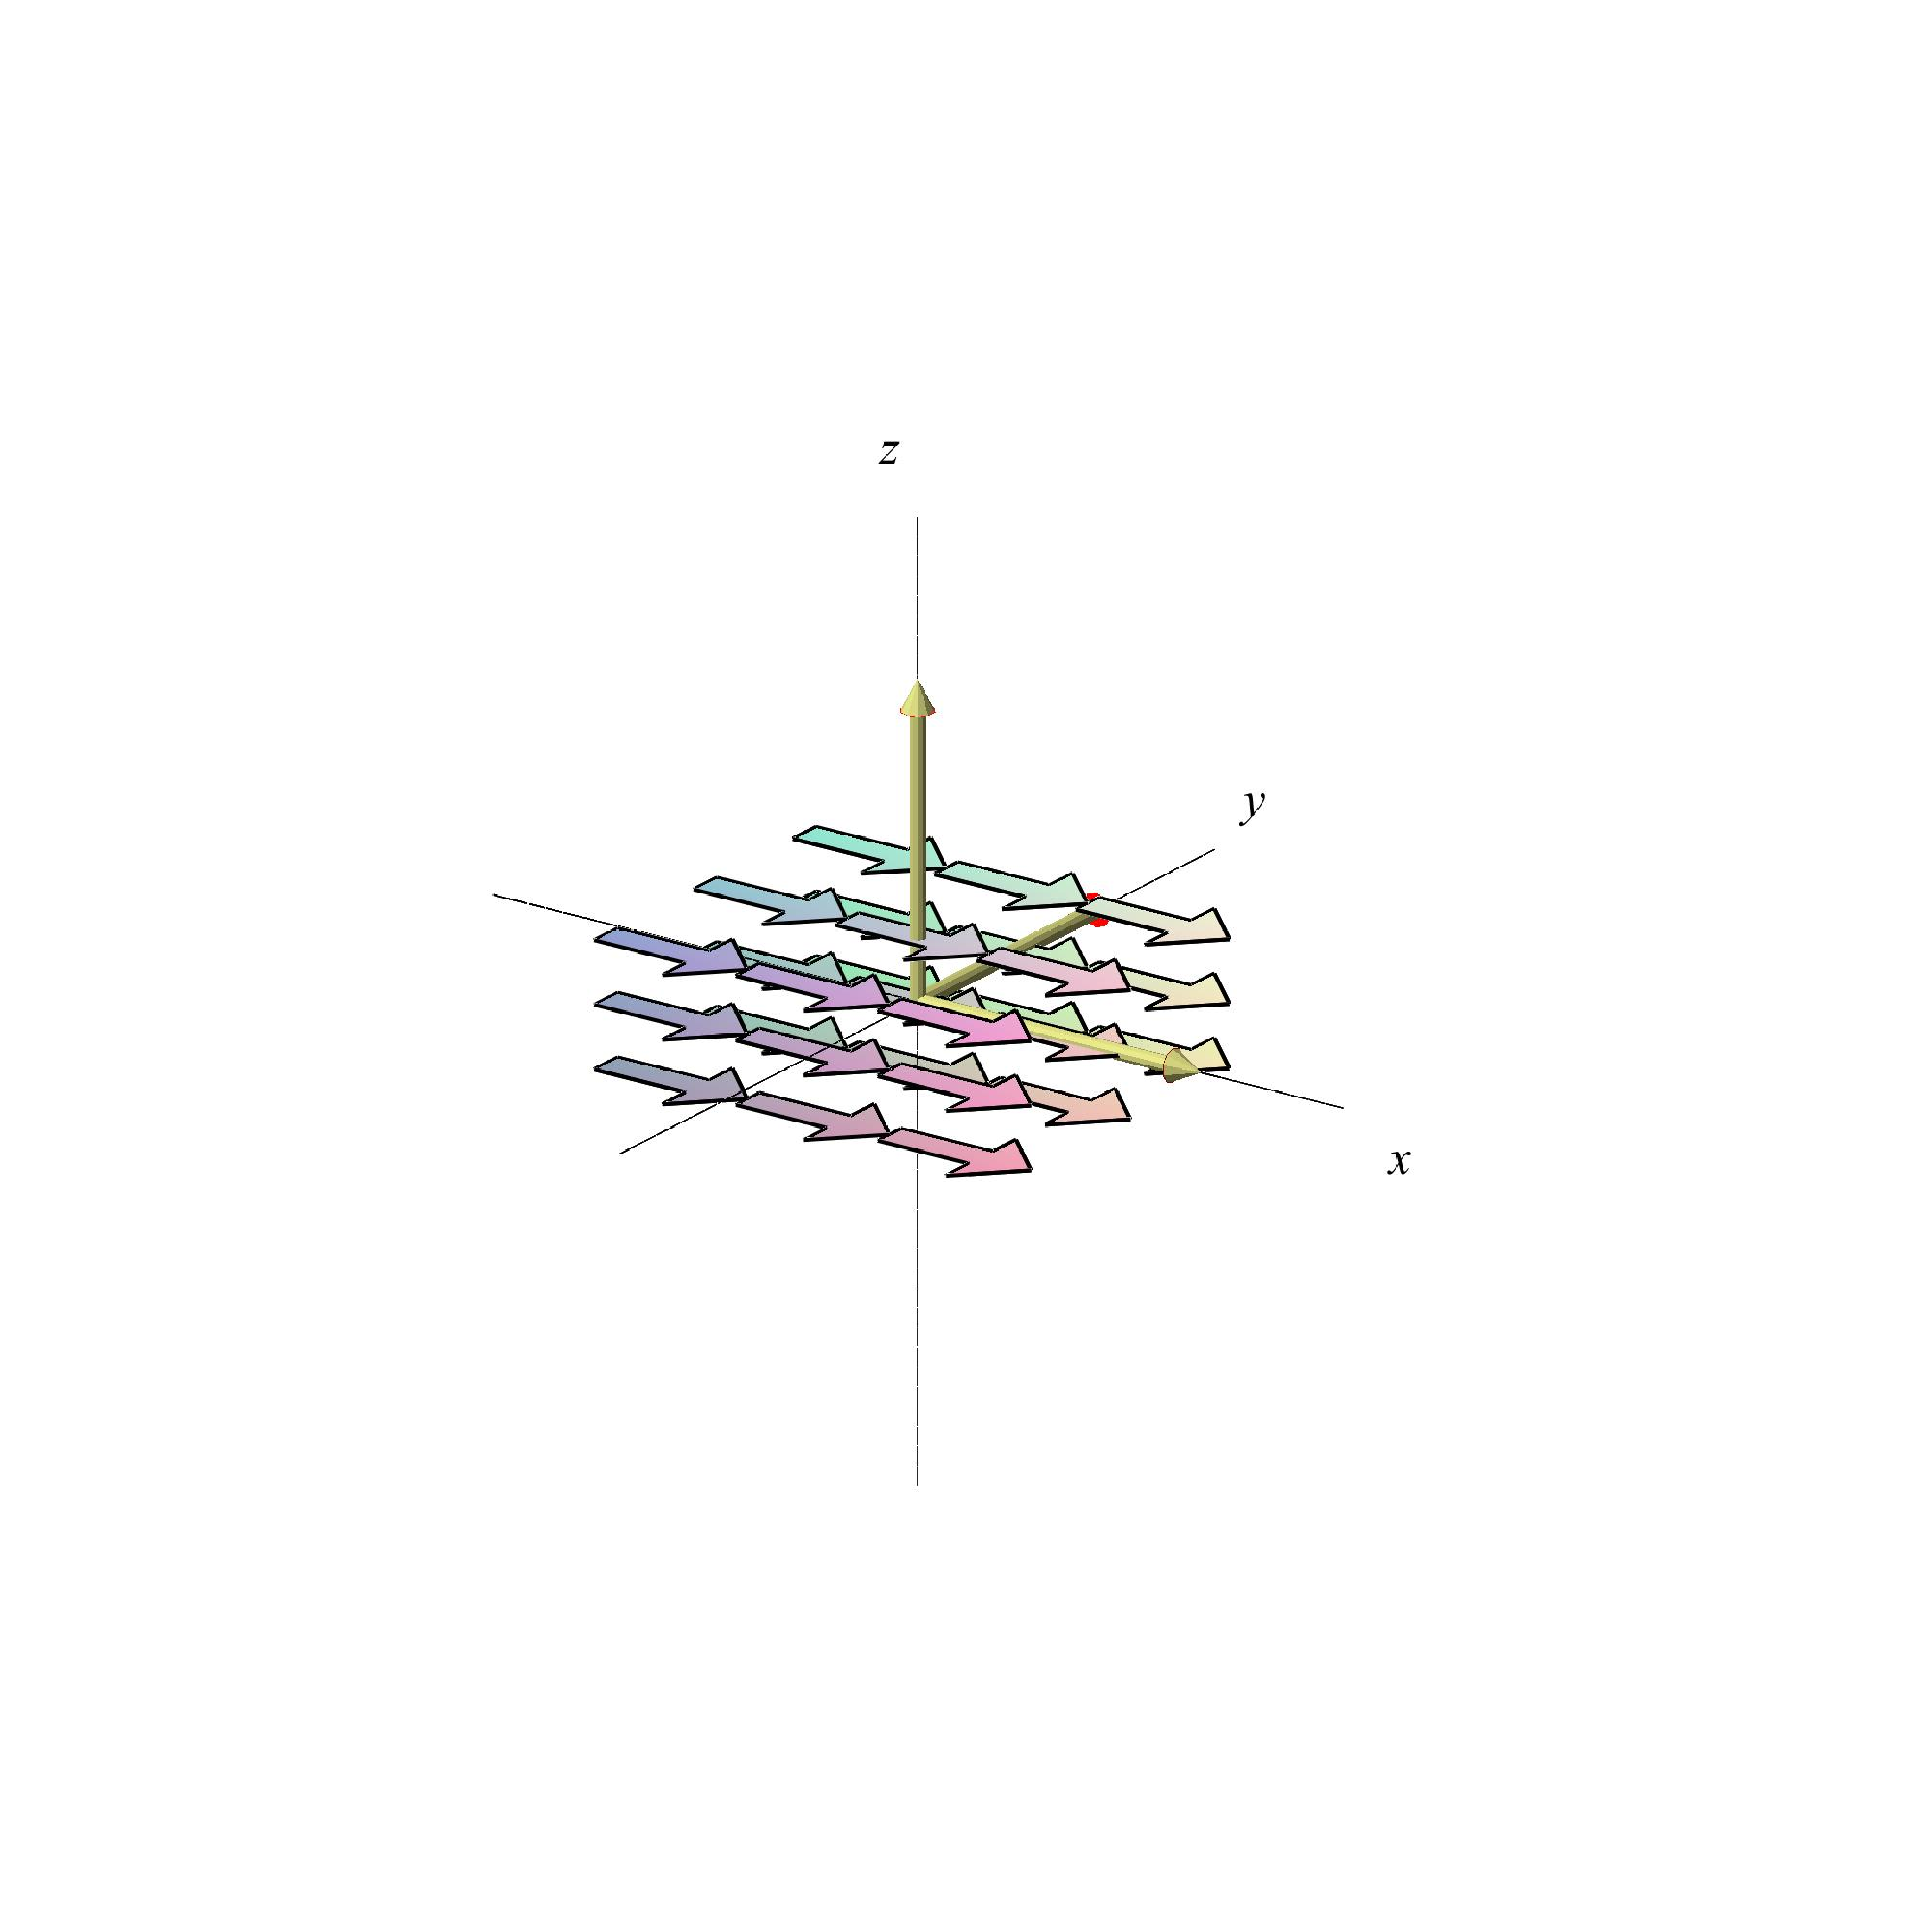
\includegraphics[height=70mm]{FIGS/plotVFUdvidet1}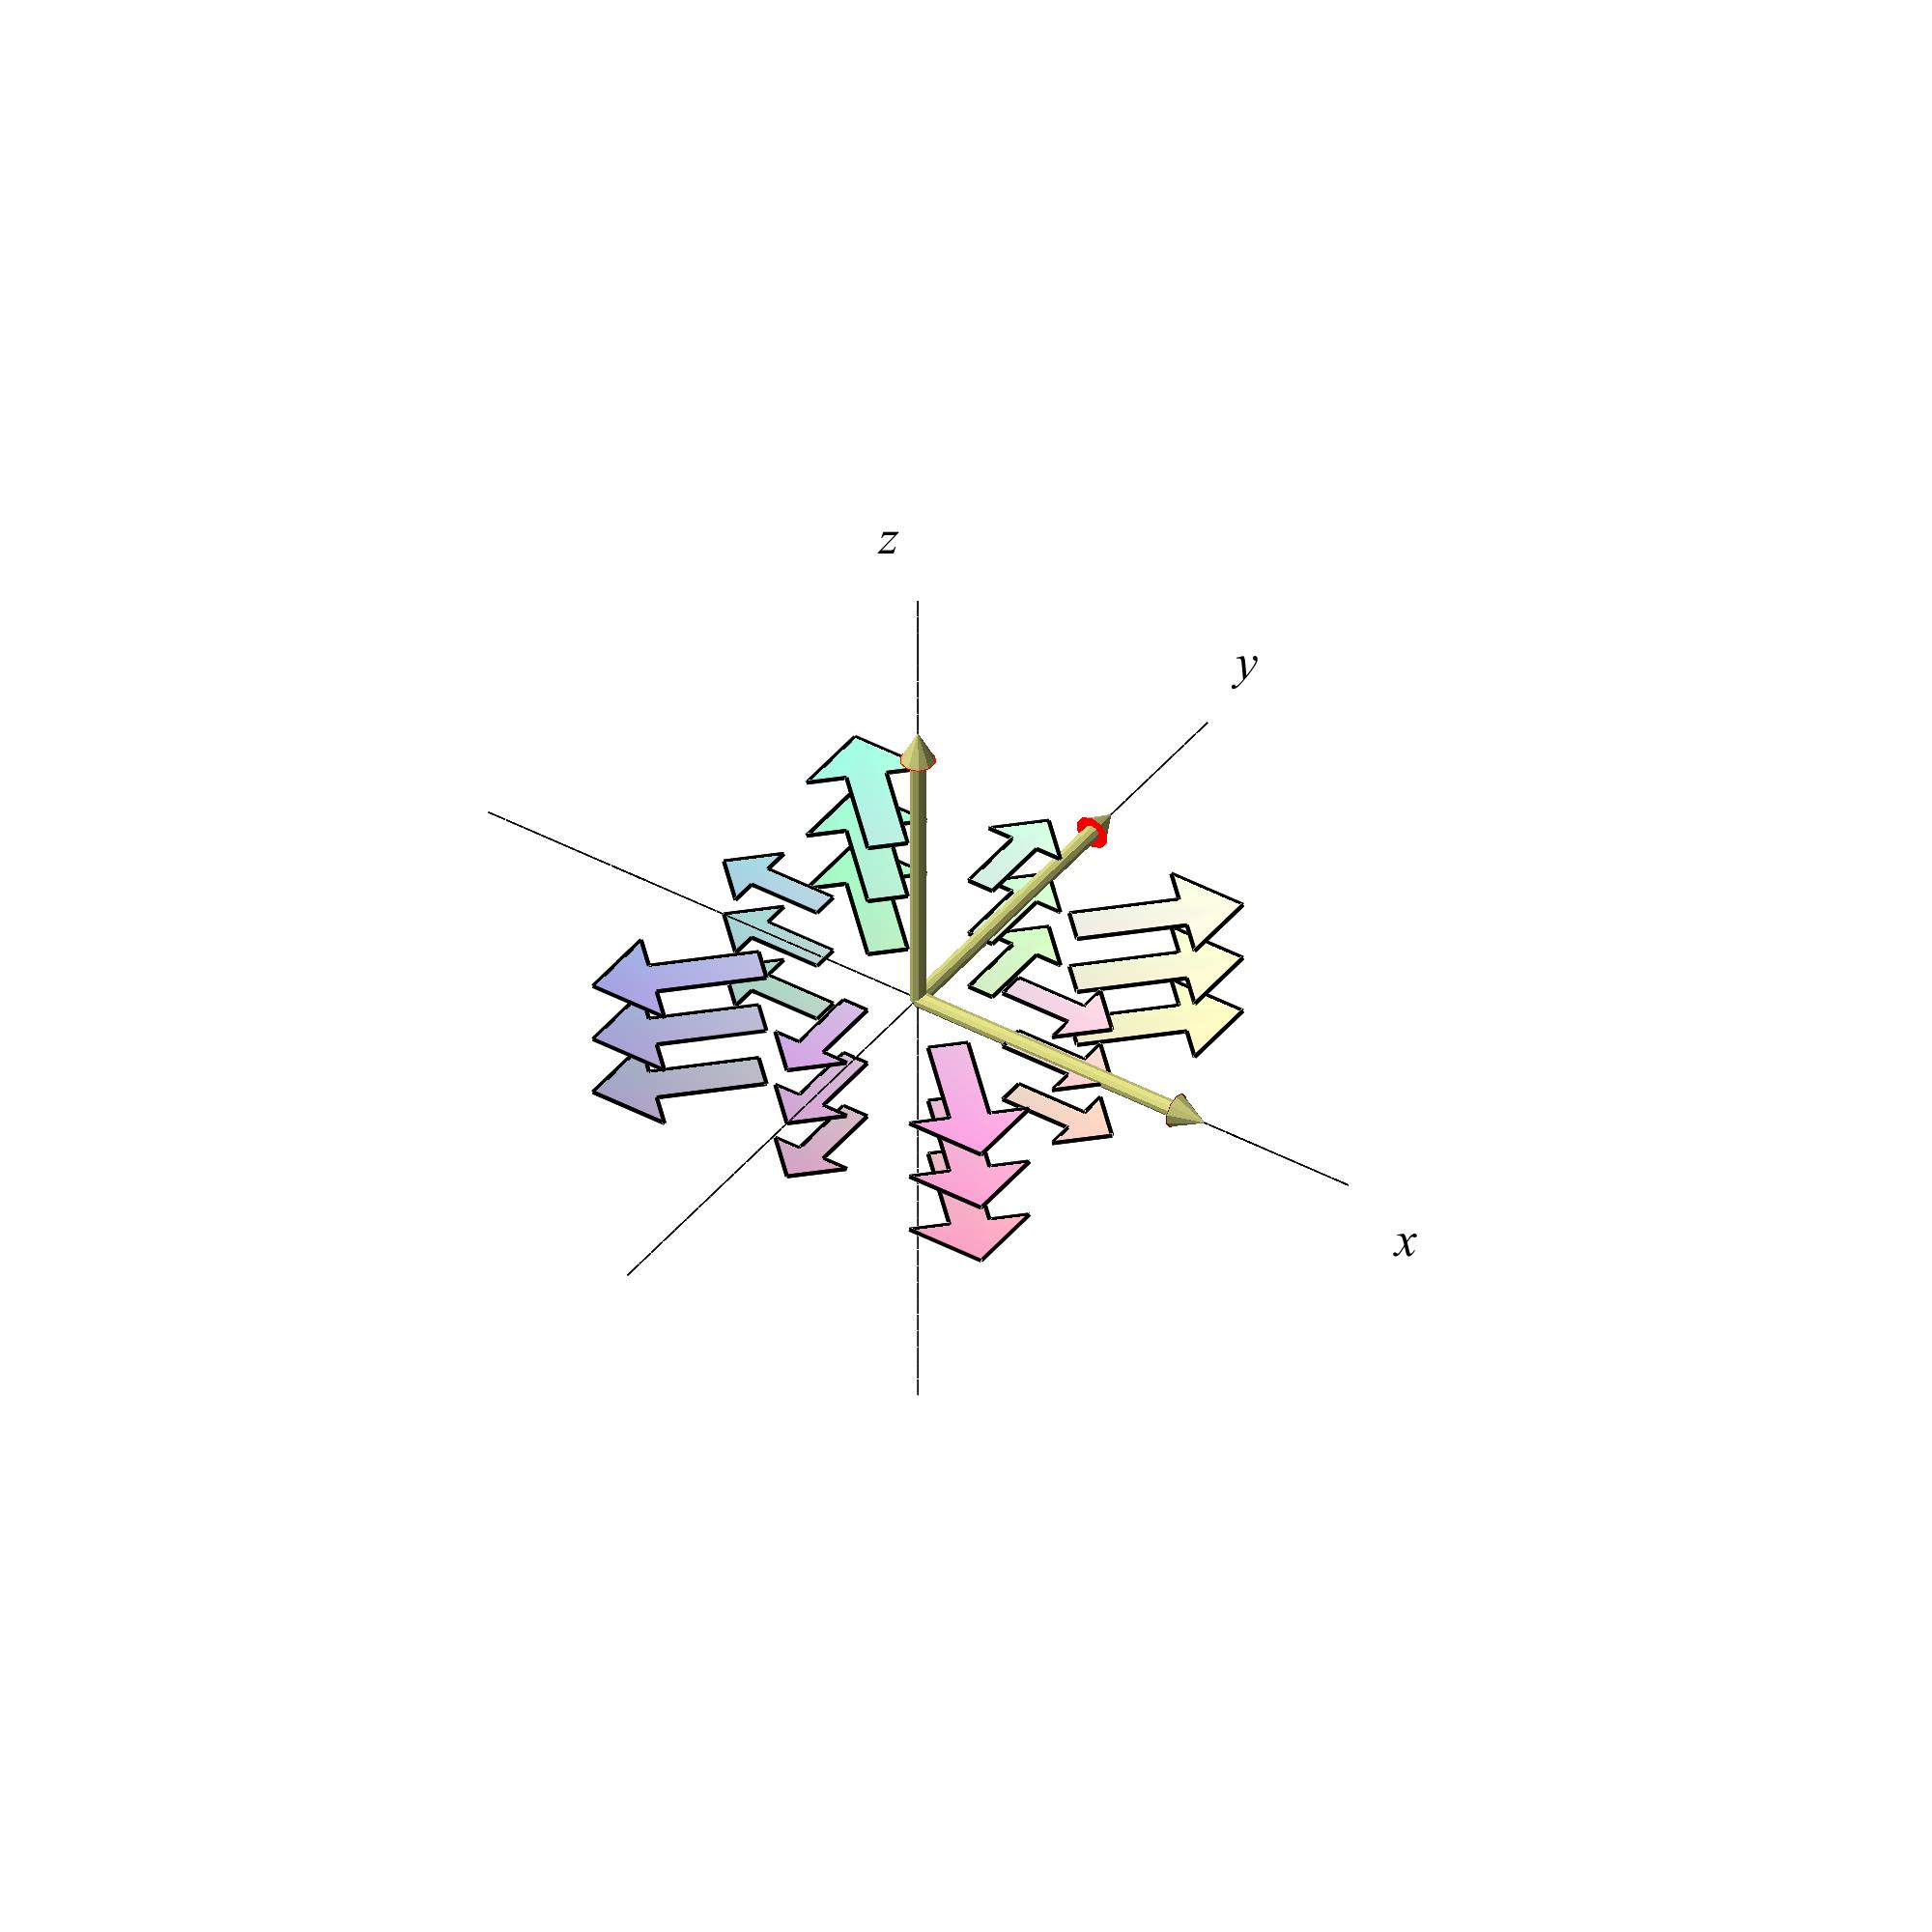
\includegraphics[height=70mm]{FIGS/plotVFUdvidet3}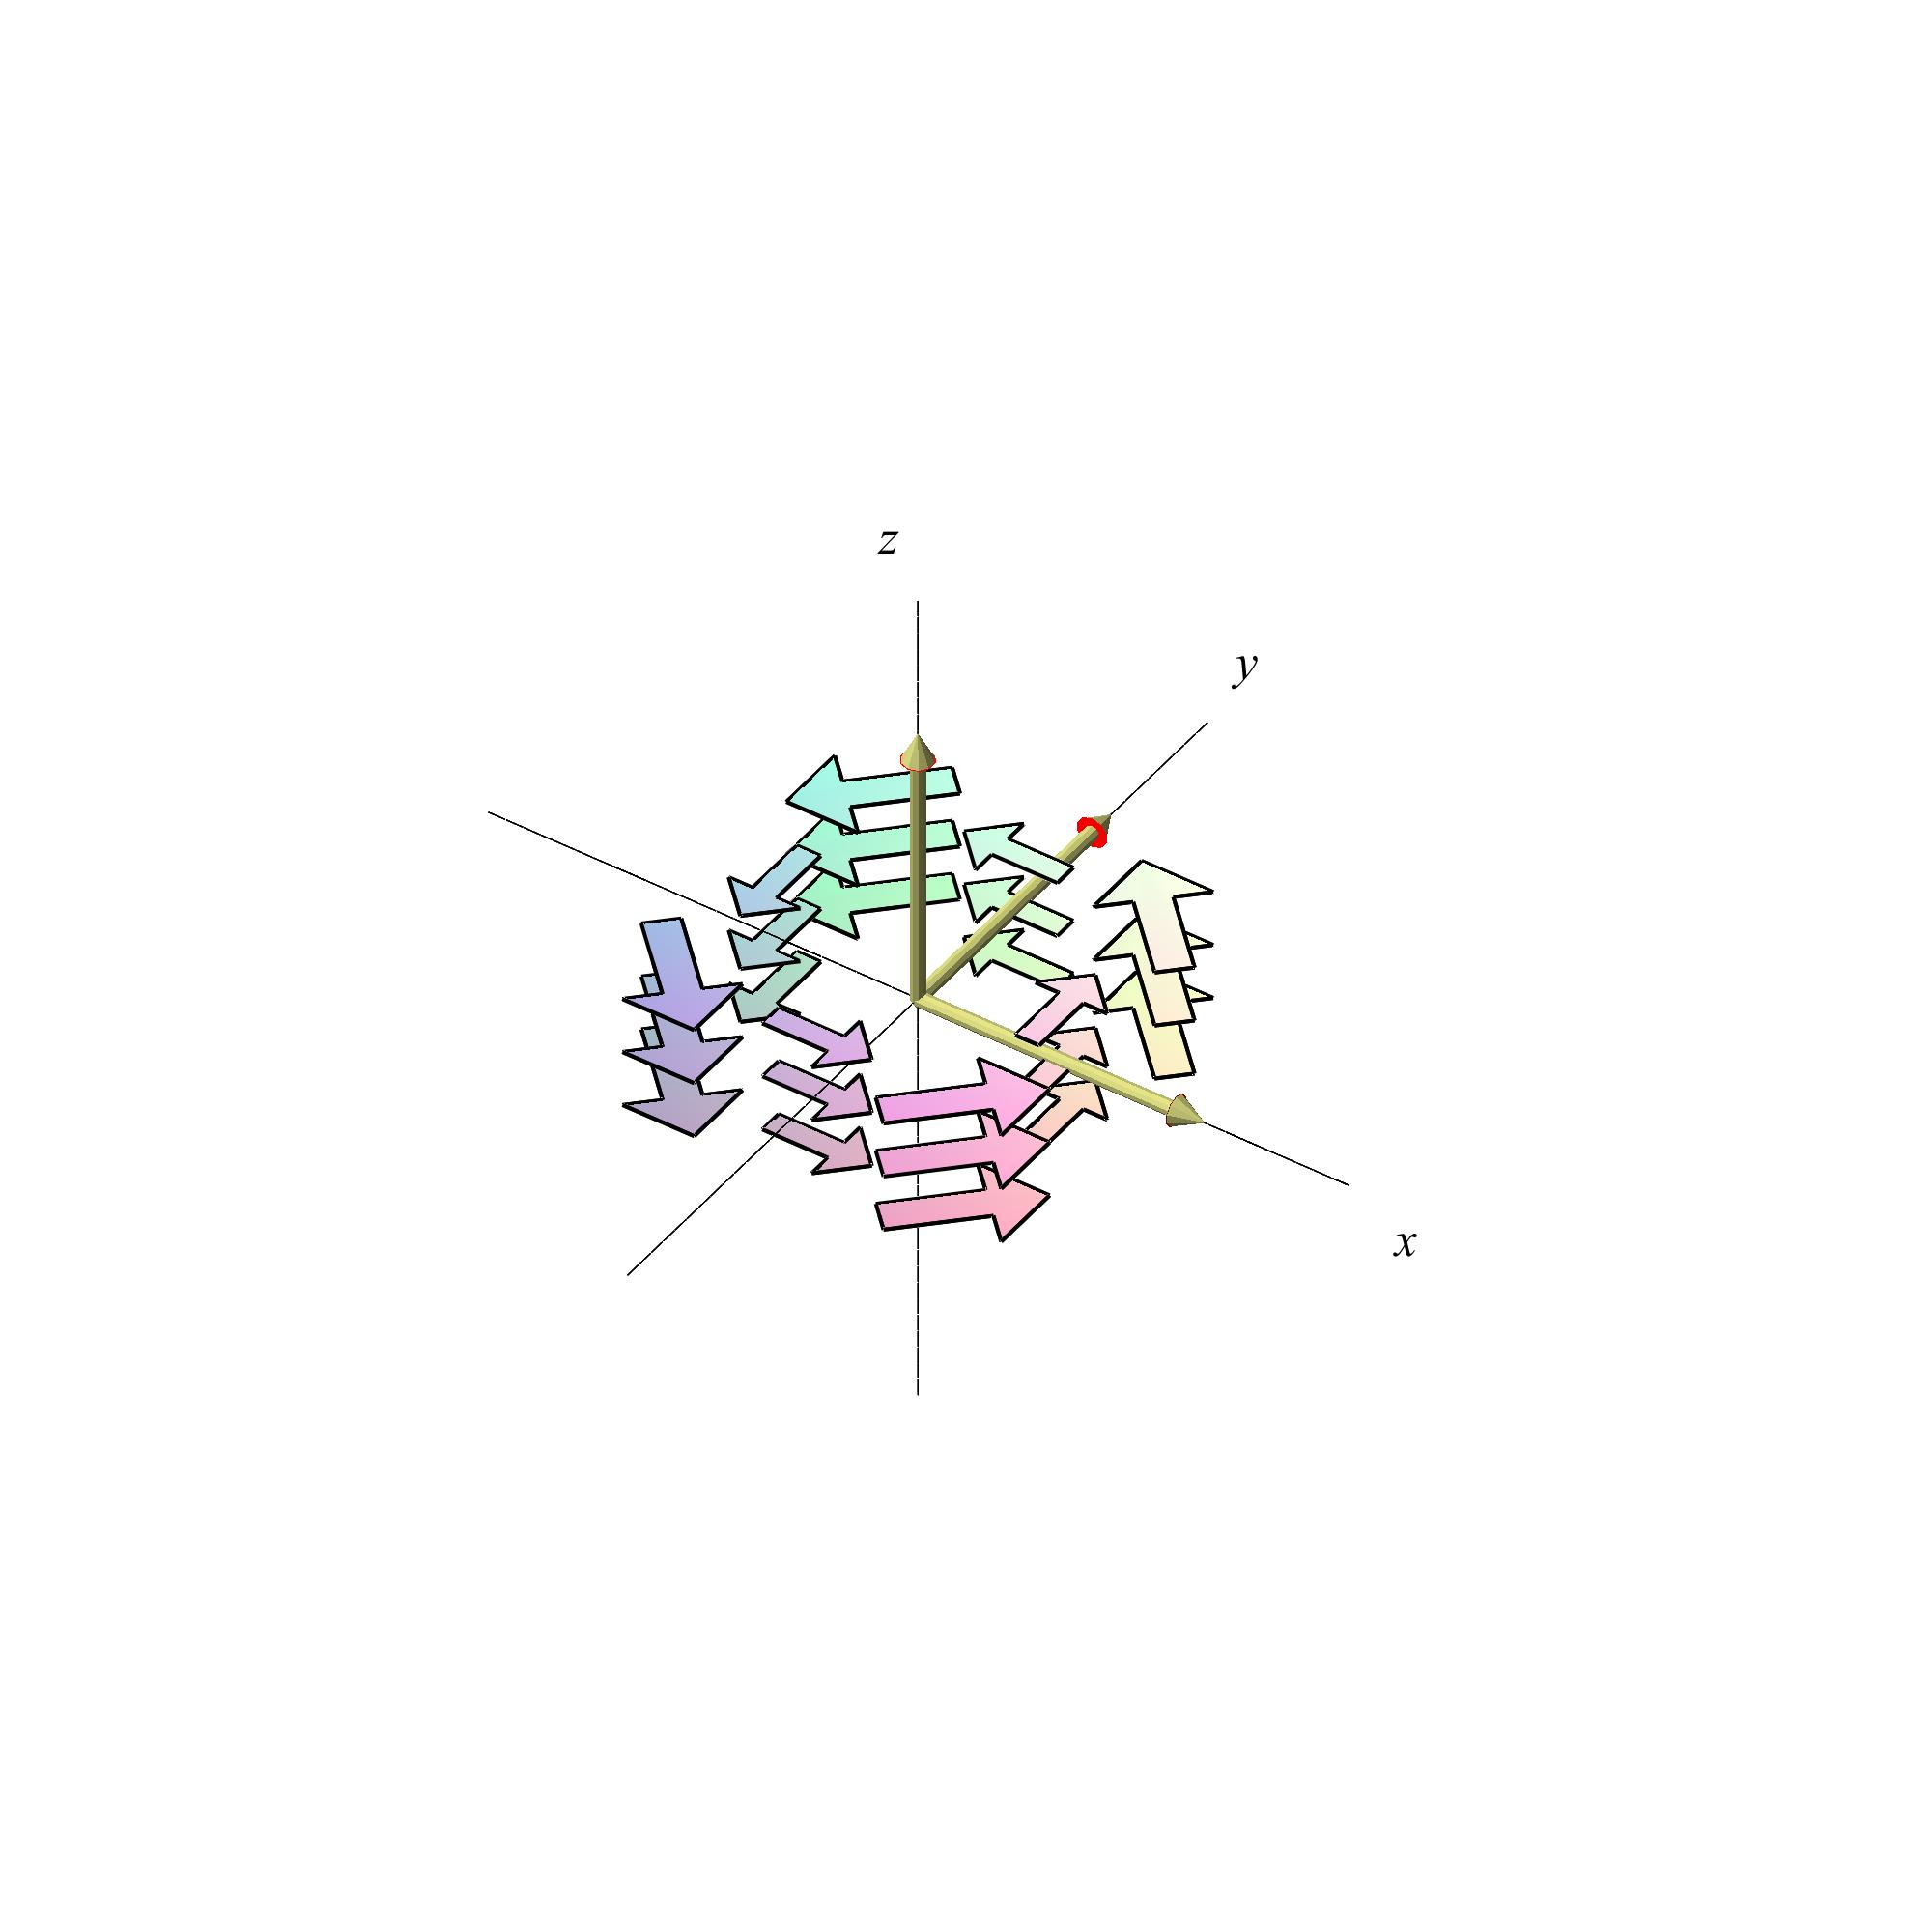
\includegraphics[height=70mm]{FIGS/plotVFUdvidet2}}
\begin{center}
\caption{\small{Tre plane vektorfelter er her udvidet til rumlige vektorfelter.}}
\label{figVFUdvidet}
\end{center}
\end{figure}


\begin{figure}[ht]
\centerline{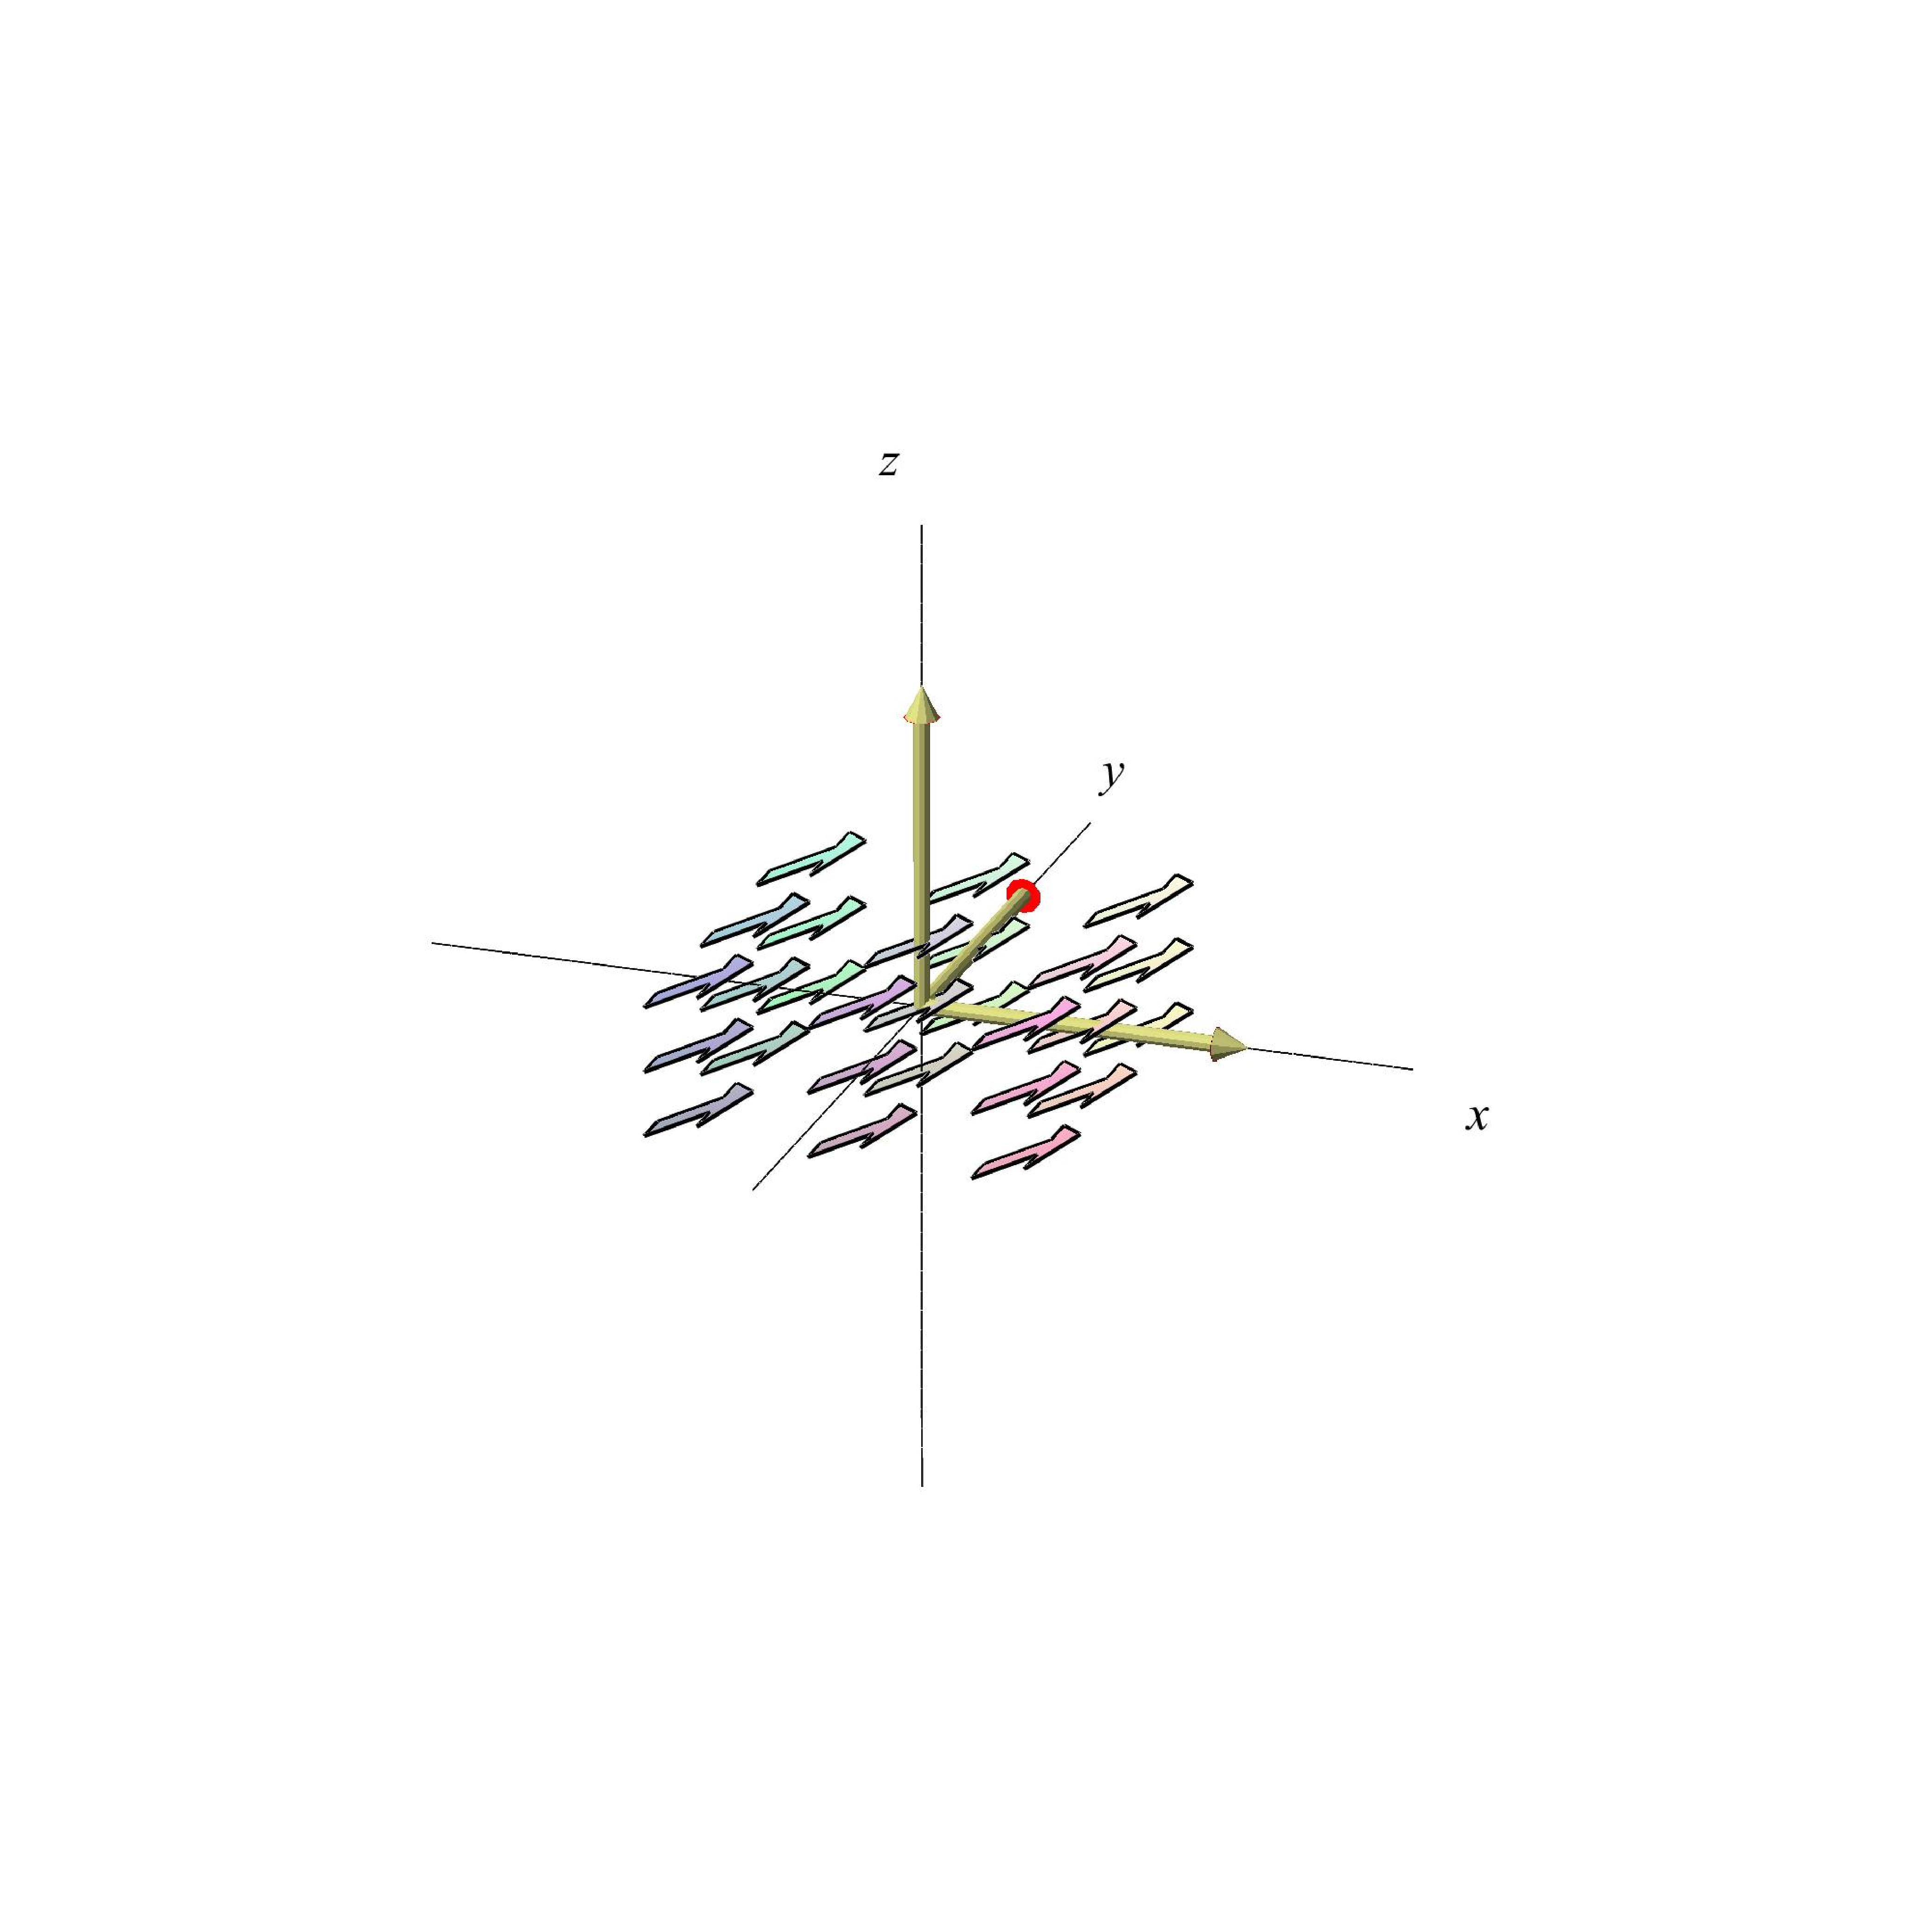
\includegraphics[height=70mm]{FIGS/plotVFUdvidet1Lift}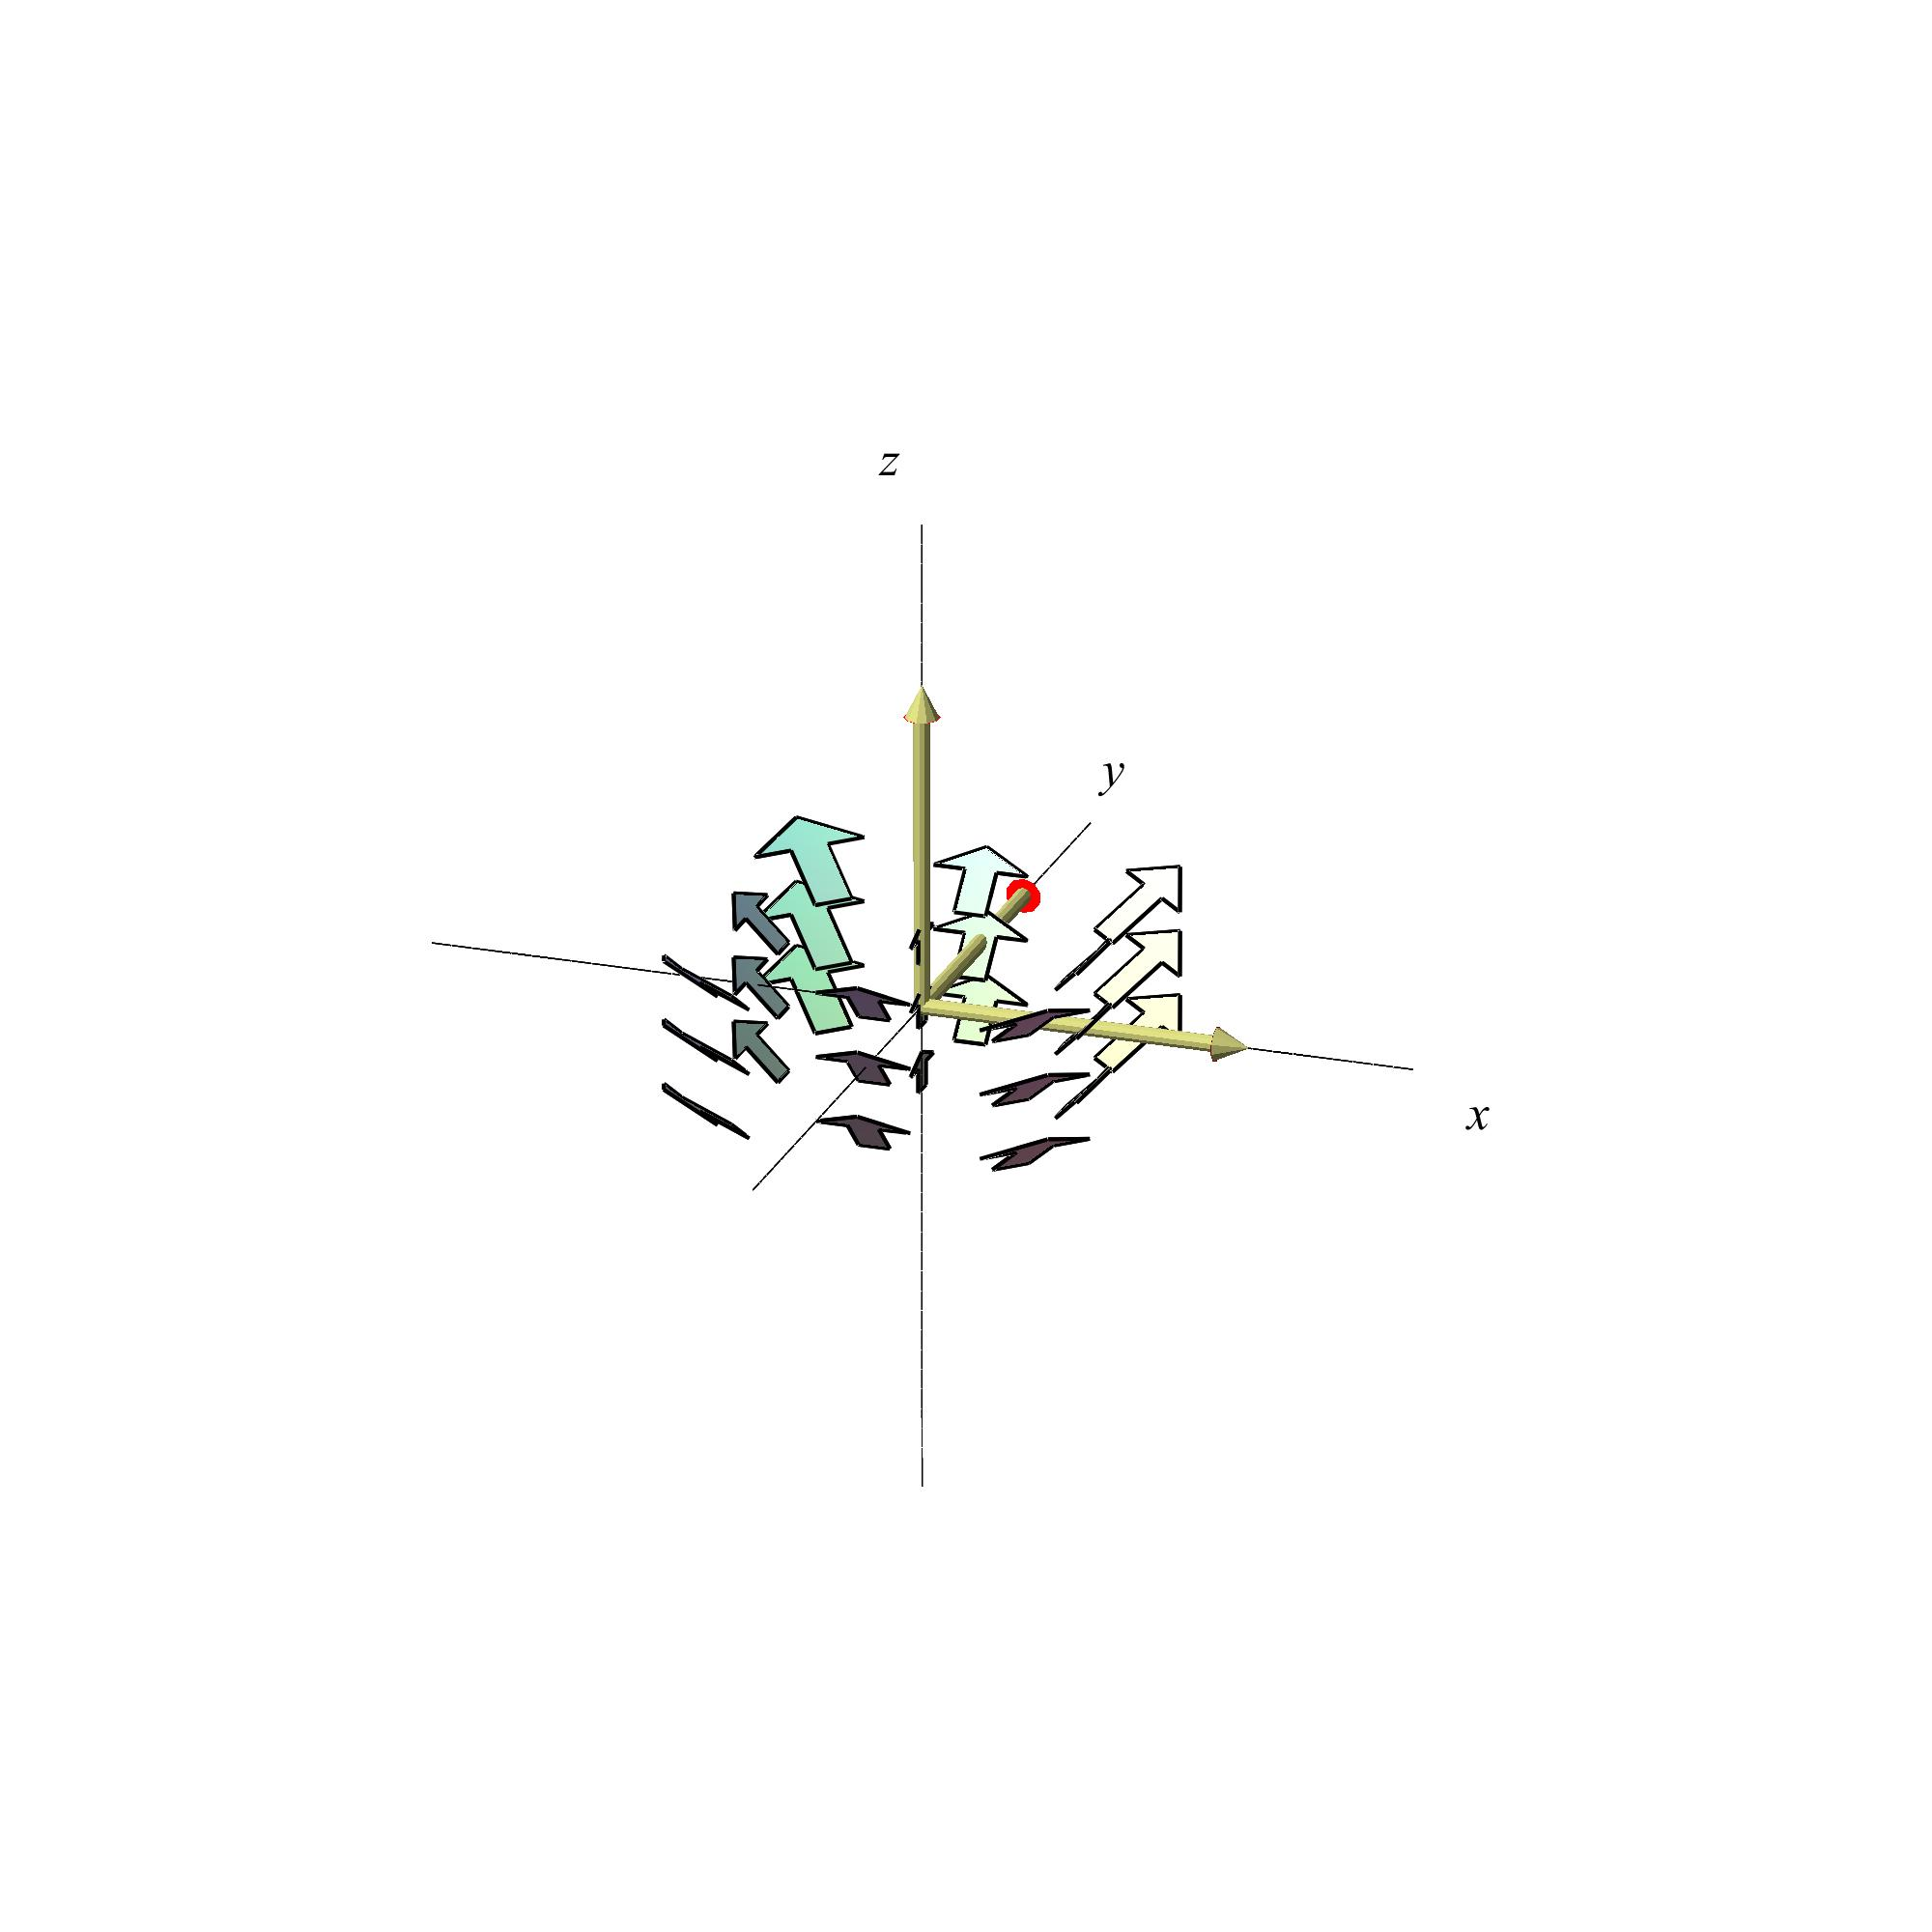
\includegraphics[height=70mm]{FIGS/plotVFUdvidet3Lift} 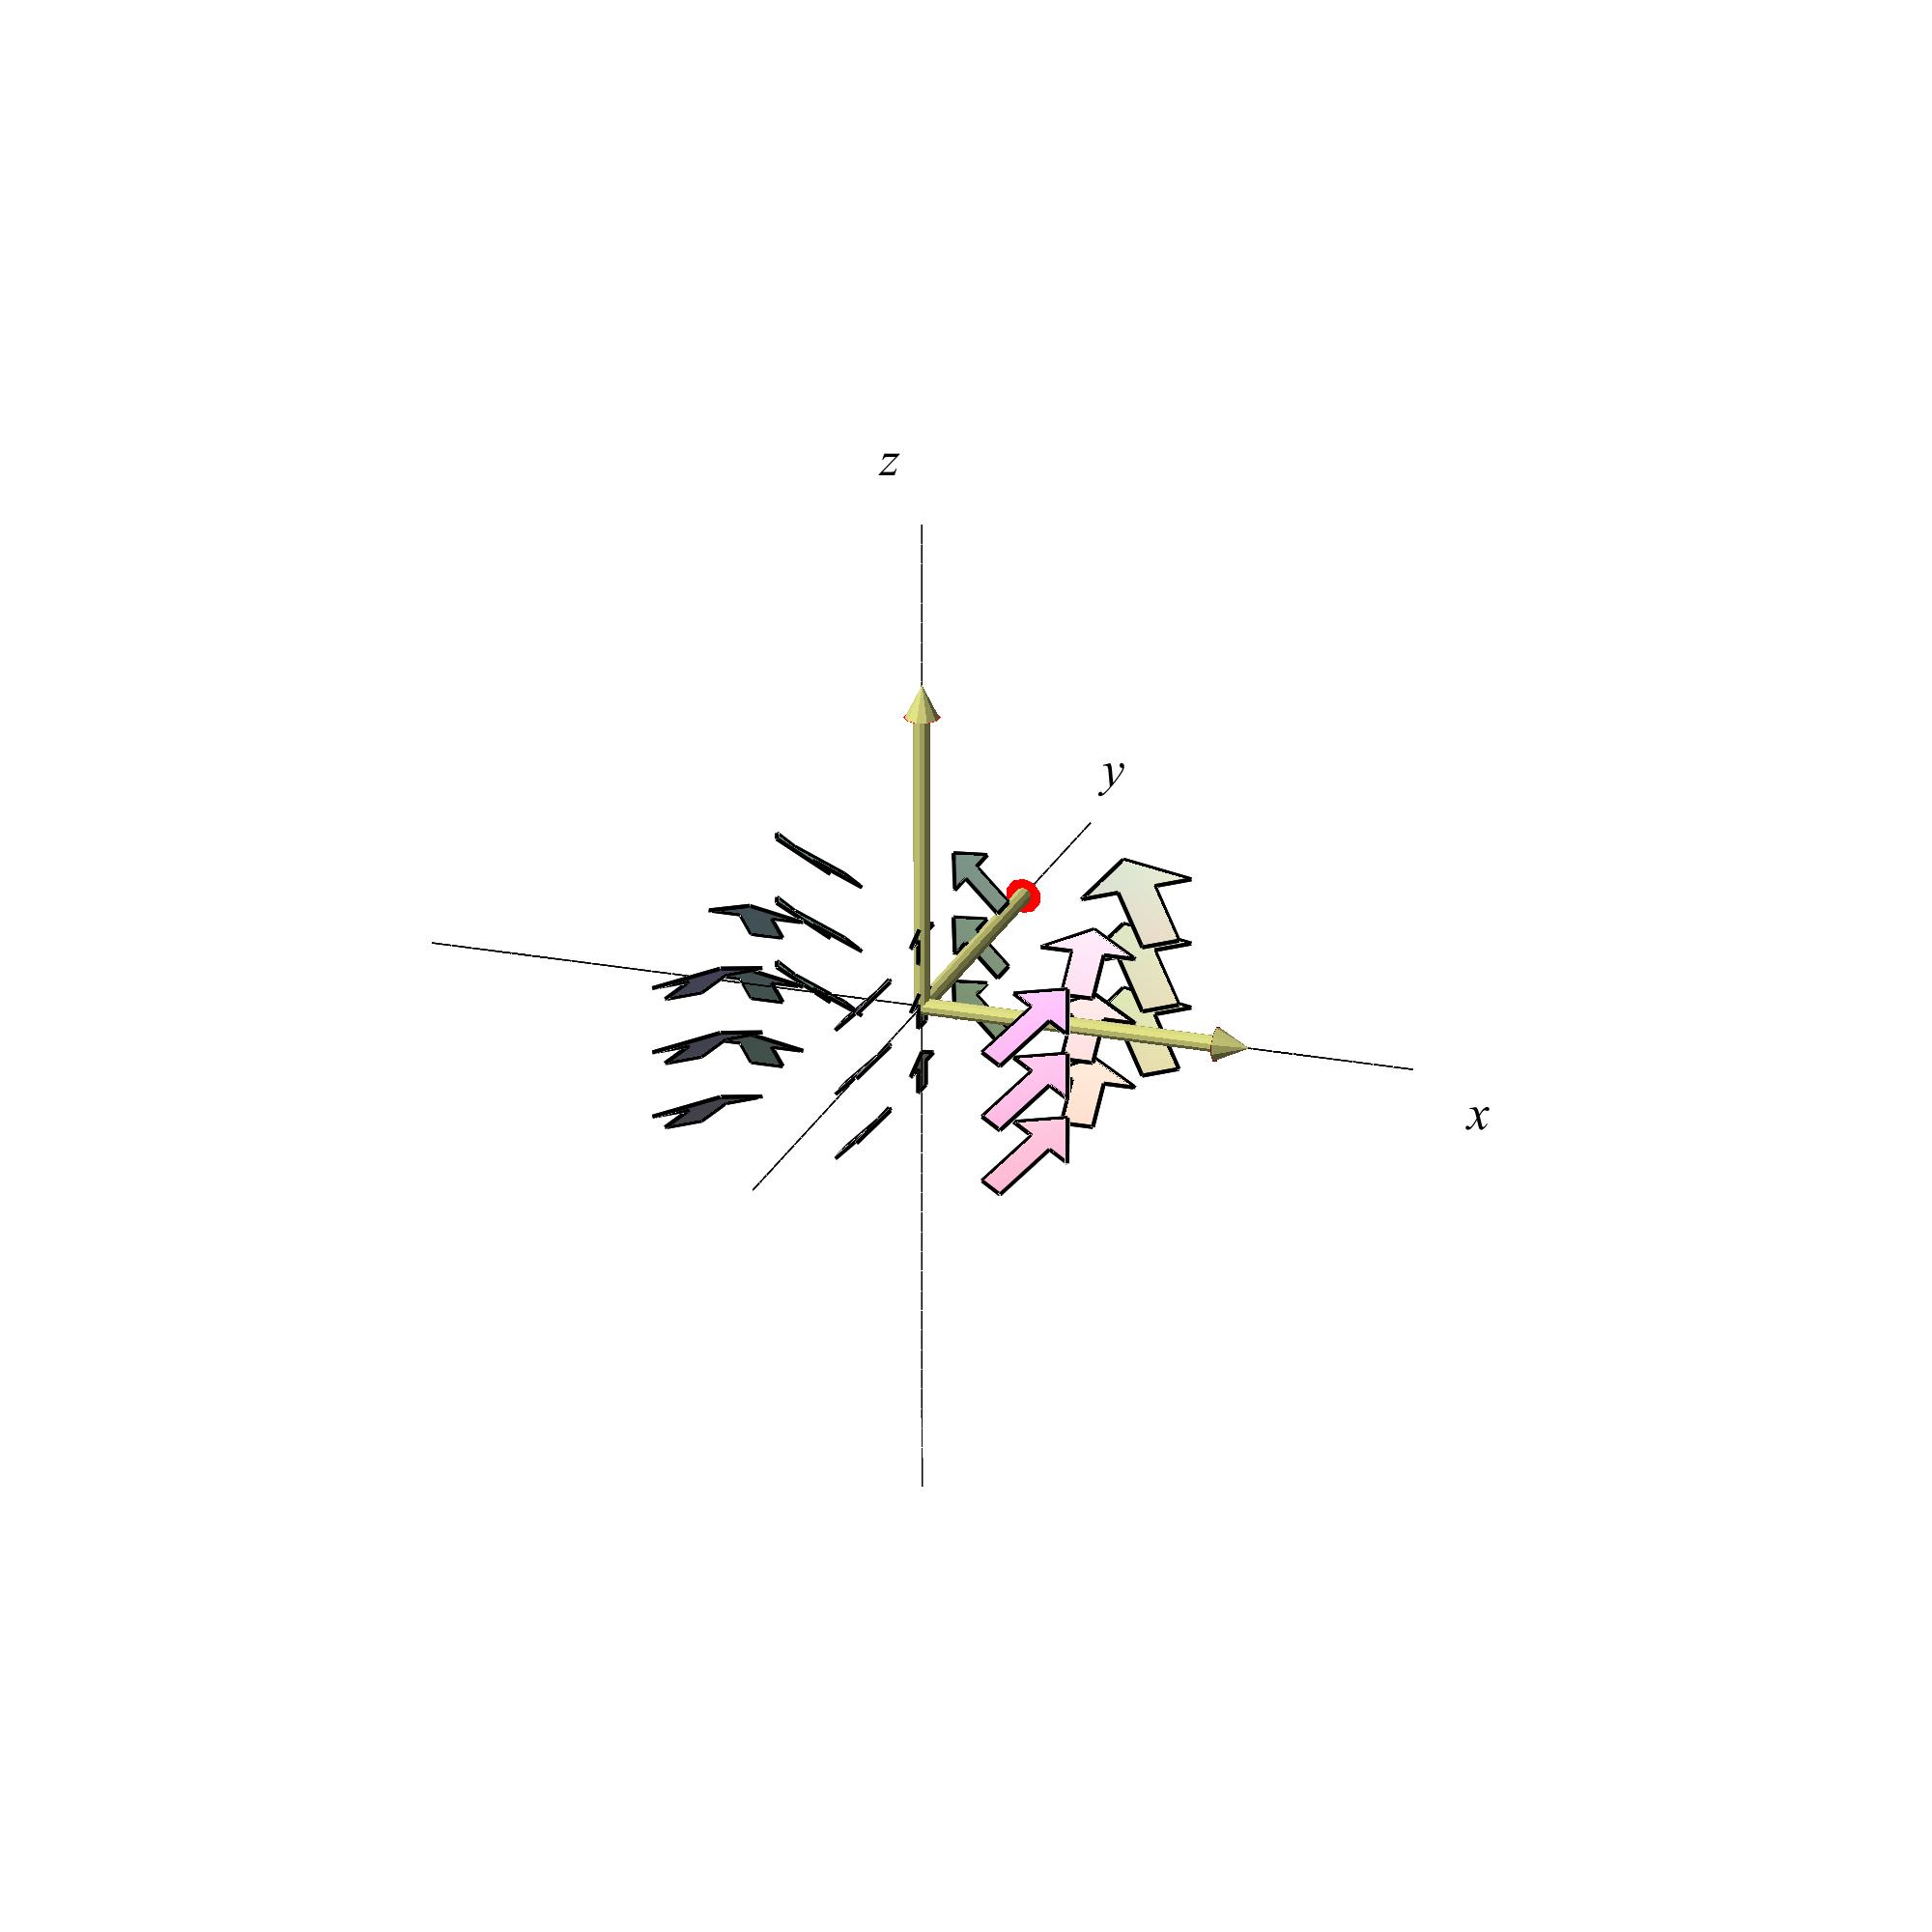
\includegraphics[height=70mm]{FIGS/plotVFUdvidet2Lift}}
\begin{center}
\caption{\small{De tre rumlige vektorfelter fra figur \ref{figVFUdvidet} er her modificerede til at have  $W_{3} = 1/2$ i stedet for $W_{3} = 0$ .}}
\label{figVFUdvidetLift}
\end{center}
\end{figure}



Nogle vektorfelter er særlig simple. Det gælder især
de vektorfelter hvor alle 3 koordinatfunktioner
er polynomier af højest første grad i de rumlige
variable $(x,y,z)$, dvs.
\begin{equation}
\begin{aligned}
{\mathbf{V}}(x,y,z) = (&a_{11}x + a_{12}y + a_{13}z + b_{1}\,\, , \\
&a_{21}x + a_{22}y + a_{23}z + b_{2}\, \, , \\   &a_{31}x + a_{32}y + a_{33}z +
b_{3}\,) \quad .
\end{aligned}
\end{equation}
I så fald kan vektorfeltet skrives kort ved hjælp af den matrix,
$\,{\mathbf{A}}\,$, der har elementerne $\,a_{ij}\,$ og den vektor,
${\mathbf{b}}$, der har koordinaterne $\,b_{i}\,$:

\begin{definition}[Vektorfelt af første grad] \label{defVFgrad1}
Et {\em{{vektorfelt  af første grad}}} er et
vektorfelt  ${\mathbf{V}}(x,y,z)$, der kan skrives på følgende form ved
hjælp af en konstant matrix ${\,\mathbf{A}\,}$ og en
konstant vektor $\,{\mathbf{b}}\,$:
\begin{equation} \label{eqVFmatrix}
{\mathbf{V}}^{\top} \, = \,  \left({\mathbf{V}}(x,y,z)\right)^{\top}\, = \,{\mathbf{A}}\cdot \left[
                                                                \begin{array}{ccc}
                                                                  x & y & z\\
                                                                \end{array}
                                                              \right]
^{\top} + \, {\mathbf{b}}^{\top} \quad ,
\end{equation}
hvor $\, \, ^{\top}$ betyder transponering af de respektive matricer, sådan at
\begin{equation}
\left[
  \begin{array}{c}
    V_{1}(x,y,z) \\
    V_{2}(x,y,z) \\
    V_{3}(x,y,z) \\
  \end{array}\right] \, = \, \left[
                        \begin{array}{ccc}
                          a_{11} & a_{12} & a_{13} \\
                          a_{21} & a_{22} & a_{23} \\
                          a_{31} & a_{32} & a_{33} \\
                        \end{array}\right]\cdot \left[
                                        \begin{array}{c}
                                          x \\
                                          y \\
                                          z \\
                                        \end{array}
                                      \right] \, + \, \left[
                                                        \begin{array}{c}
                                                          b_{1} \\
                                                          b_{2} \\
                                                          b_{3} \\
                                                        \end{array}
                                                      \right] \quad .
\end{equation}
\end{definition}



\begin{example}[Konstant vektorfelt] \label{exVFkonstant}
Et konstant vektorfelt kan for eksempel modellere en konstant vind lokalt tæt
ved $(x,y)$-planen (jord\-over\-fla\-den):
\begin{equation}
{\mathbf{V}}(x,y,z) = {\mathbf{b}} \quad ,
\end{equation}
hvor ${\mathbf{b}}$ er en konstant vektor, f.eks. ${\mathbf{b}} = (0, 7,
0)$  -- hvis vinden blæser med $7 km/t$ i $y$-aksens retning.
\end{example}


\begin{example}[Roterende vektorfelt] \label{exVFrot}
Et eksempel på et såkaldt {\emph{roterende vektorfelt}} er givet ved
\begin{equation}
{\mathbf{V}}(x,y,z) = (-y, x, 0) \quad .
\end{equation}
Se figur \ref{figVFUdvidet} i midten.
\end{example}


\begin{definition} \label{defSpor}
Sporet af en kvadratisk $n \times n$-matrix $\bm{A}$ med elementerne $a_{i\,j}$ er summen af matricens $n$ diagonalelementer:
\begin{equation}
\textbf{spor}(\bm{A}) = \sum_{i=1}^{i=n} a_{i\,i} \quad .
\end{equation}
\end{definition}


\begin{exercise}\label{exerVFrot}
Find ${\,\mathbf{A}\,}$ og $\,{\mathbf{b}}\,$ (som i Definition \ref{defVFgrad1}) for vektorfeltet i
eksempel  \ref{exVFrot}. Hvad er sporet af ${\,\mathbf{A}\,}$ i dette tilfælde tilfælde? Kan ${\,\mathbf{A}\,}$ diagonaliseres (diagonalisering beskrives i \tref{NUID3-tn4}{eNote})?
\end{exercise}


\begin{example}[Eksplosions- og implosions-vektorfelter] \label{exVFexplode}
Et eksempel på hvad vi kunne kalde et {\emph{eksplosionsvektorfelt}} er givet
ved følgende koordinatfunktioner (se hvorfor i figur \ref{figVFexplode}):
\begin{equation}
{\mathbf{V}}(x,y,z) = (x, y, z) \quad .
\end{equation}
Tilsvarende er følgende et eksempel på et vektorfelt, som vi kan kalde et \emph{implosionsvektorfelt} (se hvorfor i figur \ref{figVFimplode}):
\begin{equation}
{\mathbf{V}}(x,y,z) = (-x, -y, -z) \quad .
\end{equation}
\end{example}

\begin{exercise} \label{exerVFexplode}
Find ${\,\mathbf{A}\,}$ og $\,{\mathbf{b}}\,$ for vektorfelterne i ovenstående
eksempel \ref{exVFexplode}. Hvad er sporet af ${\,\mathbf{A}\,}$ for de to vektorfelter? Kan
${\,\mathbf{A}\,}$ diagonaliseres?
\end{exercise}

Vi vil nu begrunde de (dynamiske) navne, som vi har givet
vektorfelterne i ovenstående eksempler \ref{exVFrot} og \ref{exVFexplode}.
For at gøre det vil vi bevæge os sammen med -- eller flyde langs med -- vektorfeltet i en meget præcis forstand,
som vi nu vil definere.

%%%%%%%%%%%%%%%%%%%%%%%%%%%%%%%%%%%%%%%%%%%%%%%%%%%%%%%%%%%%%%%%%%%%%%%%%%%%%
%%%%%%%%%%%%%%%%%%%%%%%%%%%%%%%%%%%%%%%%%%%%%%%%%%%%%%%%%%%%%%%%%%%%%%%%%%%%%

\section{Flowkurver for et vektorfelt} \label{secFlow}
Lad os først repetere, at hvis vi har
givet en kurve med en parameterfremstilling
\begin{equation}
K_{\mathbf r}: \quad {\mathbf r}(t) \, = \, \left(x(t), y(t), z(t)\right)
\in \mathbb{R}^3 \quad , \, \, \,  t \in [a,b] \quad,
\end{equation}
så har denne kurve til enhver værdi af parameteren $t$  en tangentvektor nemlig
\begin{equation}
{\mathbf{r'}}(t) = (x'(t), \,y'(t),
\,z'(t))\quad .
\end{equation}
Hvis vi betragter parameteren $t\in [a,b]$ som en \emph{tids-parameter} for den
bevægelse (af en partikel)  i rummet, der er givet ved ${\mathbf r}(t)$, så er
${\mathbf{r'}}(t)$ hastigheden af partiklen til tidspunktet $t$.\\

Hvis vi konstruerer tilstrækkelig mange kurver (en kurve igennem ethvert punkt i rummet), der ikke skærer hverken sig selv eller hinanden får
vi på den måde et vektorfelt i rummet.\\

Det oplagte {\em{omvendte}} spørgsmål er nu: Givet et startpunkt $p
= (x_{0}, y_{0}, z_{0})$ og givet et vektorfelt ${\mathbf{V}}(x,y,z)$ i
rummet, findes der så en parametriseret kurve $\,{\mathbf{r}}(t)$
igennem $p$ (med $\,{\mathbf{r}}(0) = (x_{0}, y_{0}, z_{0})\,$), således
at kurvens tangentvektorfelt hele vejen {\em{langs med kurven}}
netop er det givne vektorfelt ${\mathbf{V}}(x,y,z)$ {\em{langs med
kurven}}? Hvis det er tilfældet så vil vi kalde kurven $\,{\mathbf{r}}(t)$
en \emph{integralkurve} eller en \emph{flowkurve} for vektorfeltet.
Disse
navne skyldes dels at kurven kan findes ved integration (løsning af et
differentialligningssystem) og dels at bevægelsen langs kurven er
som at flyve eller flyde  med det givne vektorfelt, altså med en fart og en
retning, som vektorfeltet angiver på ethvert sted for bevægelsen, idet kravet til bevægelsen
$\mathbf{r}(t)$  jo udtrykkes ved:

\begin{definition}[Flowkurver, Integralkurver] \label{defFlowIntKurver}
Lad $\mathbf{V}(x,y,z)$ betegne et glat vektorfelt i rummet. En parametriseret kurve
\begin{equation}
K_{\mathbf r}: \quad {\mathbf r}(t) \, = \, \left(x(t), y(t), z(t)\right) \quad , \, \, \,  t \in [a,b] \quad,
\end{equation}
kaldes en \emph{flowkurve} eller \emph{integralkurve} for vektorfeltet $\mathbf{V}(x,y,z)$ hvis ${\mathbf r}(t)$
opfylder flowkurve-ligningen:
\begin{equation}
{\mathbf{V}}(\mathbf{r}(t)) = \mathbf{r}'(t) \quad \textrm{for alle} \quad t \in [a,b]\quad ,
\end{equation}
som er ækvivalent med følgende første ordens differential-ligningssystem
\begin{equation}
\left[
  \begin{array}{c}
    x'(t) \\
    y'(t) \\
    z'(t) \\
  \end{array}
\right] = \left(\mathbf{V}(x(t), y(t), z(t))\right)^{\top} = \left[
                                                  \begin{array}{c}
                                                    V_{1}(x(t), y(t), z(t)) \\
                                                     V_{2}(x(t), y(t), z(t)) \\
                                                     V_{3}(x(t), y(t), z(t)) \\
                                                  \end{array}
                                                \right] \quad .
\end{equation}
\end{definition}


\begin{aha}
Hvis $\mathbf{V}(x,y,z)$ er givet og hvis vi har fået givet et startpunkt $p = \mathbf{r}(a)$ for en flowkurve, så er opgaven selvfølgelig den typiske, at finde løsningen til differentialligningssystemet med denne begyndelsesbetingelse, dvs. finde koordinatfunktionerne $x(t)$, $y(t)$, og $z(t)$ således at $p = (x(a), y(a), z(a))$. \\

Med andre ord:
Hvis vi har givet et vektorfelt i rummet så går opgaven ud på at starte en bevægelse af en partikel (en lille kugle) langs vektorfeltet
sådan at kuglens hastighedsvektor til ethvert tidspunkt er givet ved vektorfeltets værdi i det punkt hvor kuglen befinder sig til det tidspunkt.
Og det er naturligvis interessant at kunne afgøre \emph{hvor} kuglen befinder sig efter lang tid. Og det er interessant at finde ud af, hvordan en kugle-hob
(partikler som til start er tæt på hinanden) udvikler sig i tiden -- bliver hoben tættere eller tyndere, mast sammen eller trukket ud?
\end{aha}


Der gælder følgende eksistens- og entydighedssætning som er grundlaget for vore første eksempler og de første overvejelser om de naturlige spørgsmål der vedrører flowkurver og deres opførsel.

\begin{theorem}[Eksistens og entydighedssætningen] \label{thmVFgrad1}
Lad  $\,{\mathbf{V}}(x,y,z)\,$ være et vektorfelt af  \emph{første grad},  givet ved en koefficientmatrix $\mathbf{A}$ og en vektor $\mathbf{b}$ som i definition \ref{defVFgrad1}. Lad
 $\,(x_{0}, y_{0}, z_{0})\,$ betegne et vilkårligt punkt i rummet. Så
findes der netop \'{e}n kurve $\,{\mathbf{r}}(t)$,
der opfylder de to betingelser:
\begin{equation}\label{eqDifSystVF}
\begin{aligned}
\,{\mathbf{r}}(0) \, &= \, (x_{0}, y_{0}, z_{0}) \quad  {\rm{og}} \\ \\
\,{\mathbf{r}}\,'(t)\, &= \,{\mathbf{V}}(x(t), y(t), z(t)) \quad  {\rm{for}}\quad  {\rm{alle}} \quad
 t \in [-\infty, \infty] \quad .
\end{aligned}
\end{equation}
Den sidste ligning (\ref{eqDifSystVF})  er ækvivalent med følgende differentialligningssystem med en konstant koefficientmatrix $\mathbf{A}$:
\begin{equation}
\begin{aligned}
\left[
  \begin{array}{c}
    x'(t) \\
    y'(t) \\
    z'(t) \\
  \end{array}
\right] &= \left(\mathbf{V}(x(t), y(t), z(t))\right)^{\top}\\
 &= \mathbf{A}\cdot \left[
                                                                               \begin{array}{ccc}
                                                                                 x(t) & y(t) & z(t) \\
                                                                               \end{array}
                                                                             \right]^{\top} + \mathbf{b}^{\top} \\
&=
 \left[
                        \begin{array}{ccc}
                          a_{11} & a_{12} & a_{13} \\
                          a_{21} & a_{22} & a_{23} \\
                          a_{31} & a_{32} & a_{33} \\
                        \end{array}\right]\cdot \left[
                                        \begin{array}{c}
                                          x(t) \\
                                          y(t)\\
                                          z(t) \\
                                        \end{array}
                                      \right] \, + \, \left[
                                                        \begin{array}{c}
                                                          b_{1} \\
                                                          b_{2} \\
                                                          b_{3} \\
                                                        \end{array}
                                                      \right] \quad .
\end{aligned}
\end{equation}
\end{theorem}

Hvis vi har givet et vektorfelt af  første
grad, så kan vi altså ''starte'' et punkt, en partikel, et vilkårligt sted i rummet og lade den ''flyde'' med vektorfeltet sådan at partiklen
befinder sig på en entydigt bestemt flowkurve til enhver tid derefter.

\begin{aha}
To flowkurver kan ikke skære hinanden, fordi hvis de gjorde det ville der jo ikke være en \emph{entydig} flowkurve igennem skæringspunktet.
\end{aha}

\begin{info}
Sætningen kan udvides til vektorfelter der ikke
nødvendigvis er af  første grad, men så er
det ikke længere sikkert, at alle
tids-parameterintervallerne for flowkurverne er
hele det dobbeltuendelige interval $\,\mathbb{R}= ]-\infty,
\infty[\,$. Integralkurverne for et vektorfelt af
 første grad kan findes og vises med
Maple og er eksemplificeret i
figurerne \ref{figVFrot}, \ref{figVFexplode}, og
\ref{figVFimplode}. \\

Hvis vektorfeltet ikke er af
 første grad er der som sagt ingen garanti
for, at flowkurverne kan bestemmes explicit (heller ikke
med Maple), men i visse tilfælde kan numeriske værktøjer jo
alligevel benyttes med succes indenfor de ''vinduer'' hvor løsningerne findes og er veldefinerede.
\end{info}

Begrundelsen, beviset, for sætning
\ref{thmVFgrad1} er kendt fra studiet af systemer af lineære
koblede differentialligninger, se \tref{NUID13-tn12}{eNote}. Lad os kort
repetere de overvejelser, der skal i sving ved at finde flowkurverne for nogle af de simpleste vektorfelter.

\begin{example}[Flowkurver for et konstant vektorfelt]\label{exVFkonstantFlow}
Det konstante vektorfelt ${\mathbf{V}}(x,y,z) = (0,7,0)$ har flowkurver
$(x(t), y(t), z(t))$ som skal opfylde de to betingelser:
Begyndelsebetingelsen $(x(0), y(0), z(0)) = (x_{0}, y_{0}, z_{0})$
og de $3$ differentialligninger for $x(t)$, $y(t)$, og $z(t)$, som
følger af hastighedsvektor-betingelsen
\begin{equation}
{\mathbf{r}}'(t) = (x'(t),
y'(t), z'(t)) = {\mathbf{V}}(x(t), y(t), z(t)) = (0, 7, 0) \quad .
\end{equation}
Opgaven er at finde de tre koordinatfunktioner  $x(t)$, $y(t)$, og $z(t)$ sådan at
\begin{equation}
\begin{aligned}
x'(t) &= 0 \\
y'(t) &=  7 \\
z'(t) &= 0  \quad .
\end{aligned}
\end{equation}
De 3
differentialligninger er i dette tilfælde ikke koblede og de løses
direkte med de angivne begyndelsebetingelser med følgende resultat:
$x(t) = x_{0}$, $y(t) = y_{0} + 7\,t$, og $z(t) = z_{0}$. Dvs.
flowkurverne er (ikke overraskende) alle de rette linjer parallelle
med $y$-aksen, parametriseret sådan at alle har farten $7$.
\end{example}


\begin{example}[Flowkurver for et roterene vektorfelt]\label{exVFrotFlow}
Eksemplet med det roterende vektorfelt $
{\mathbf{V}}(x,y,z) = (-y, x, 1)$ har tilsvarende
flow\-kurver, der nu tilfredsstiller
betingelserne: $(x(0), y(0), z(0)) = (x_{0},
y_{0}, z_{0})$ samt differential\-lig\-nin\-gerne
\begin{equation}
{\mathbf{r}}'(t) = (x'(t), y'(t), z'(t)) = (-y(t), x(t), 1) \quad.
\end{equation}
Opgaven er altså her at finde de tre koordinatfunktioner  $x(t)$, $y(t)$, og $z(t)$ sådan at
\begin{equation}
\begin{aligned}
x'(t) &= -y(t) \\
y'(t) &=  x(t) \\
z'(t) &=  1 \quad .
\end{aligned}
\end{equation}

Differentialligningerne for $x(t)$ og
$y(t)$ er koblede lineære differentialligninger
med konstante koefficienter og løses præcis som i
 \tref{NUID13-tn12}{eNote} . Bemærk, at systemmatricen
allerede er fundet i opgave \ref{exerVFrot}.
Resultatet er $x(t) = x_{0}\cos(t) -
y_{0}\sin(t)\,$, $y(t) =
x_{0}\sin(t)+y_{0}\cos(t)\,$, og $z(t) = z_{0} +
t$. Disse flowkurver kan findes og inspiceres med
Maple. Det fremgår også
deraf at det er ganske rimeligt at kalde
vektorfeltet et roterende vektorfelt. Se figur
\ref{figVFrot}.
\end{example}


\begin{figure}[h]
\centerline{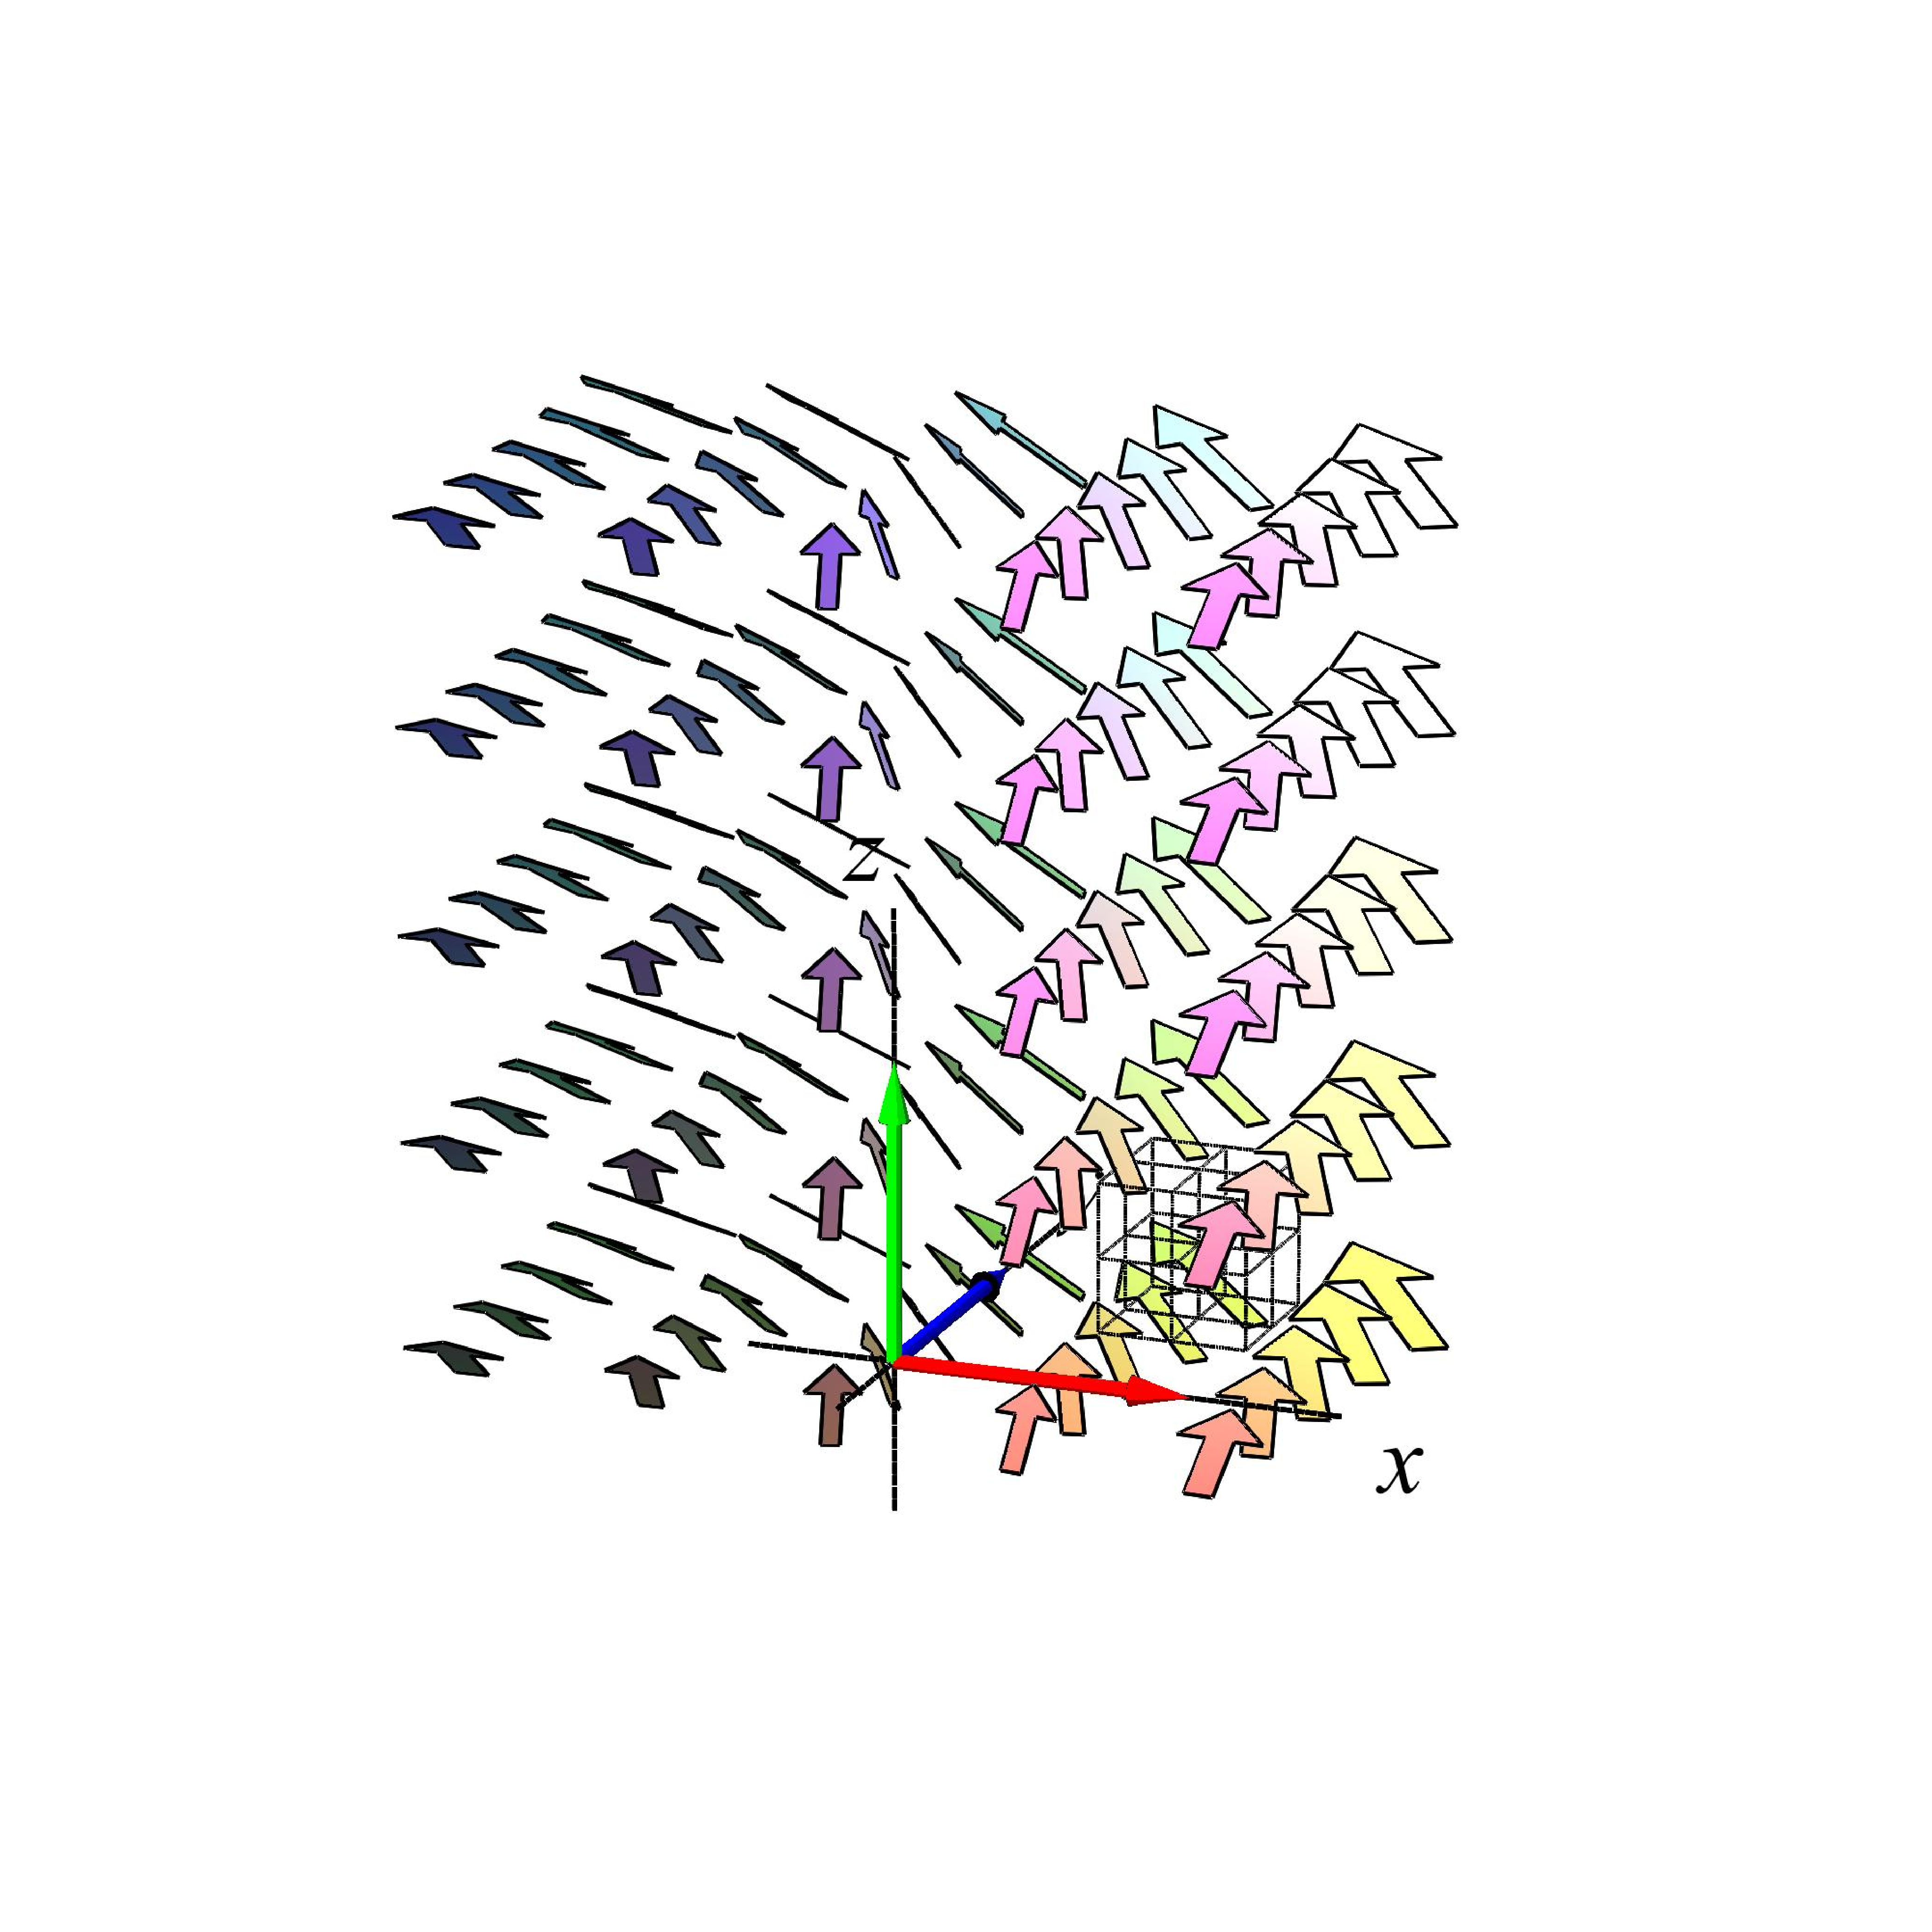
\includegraphics[height=70mm]{FIGS/plotVFrot1}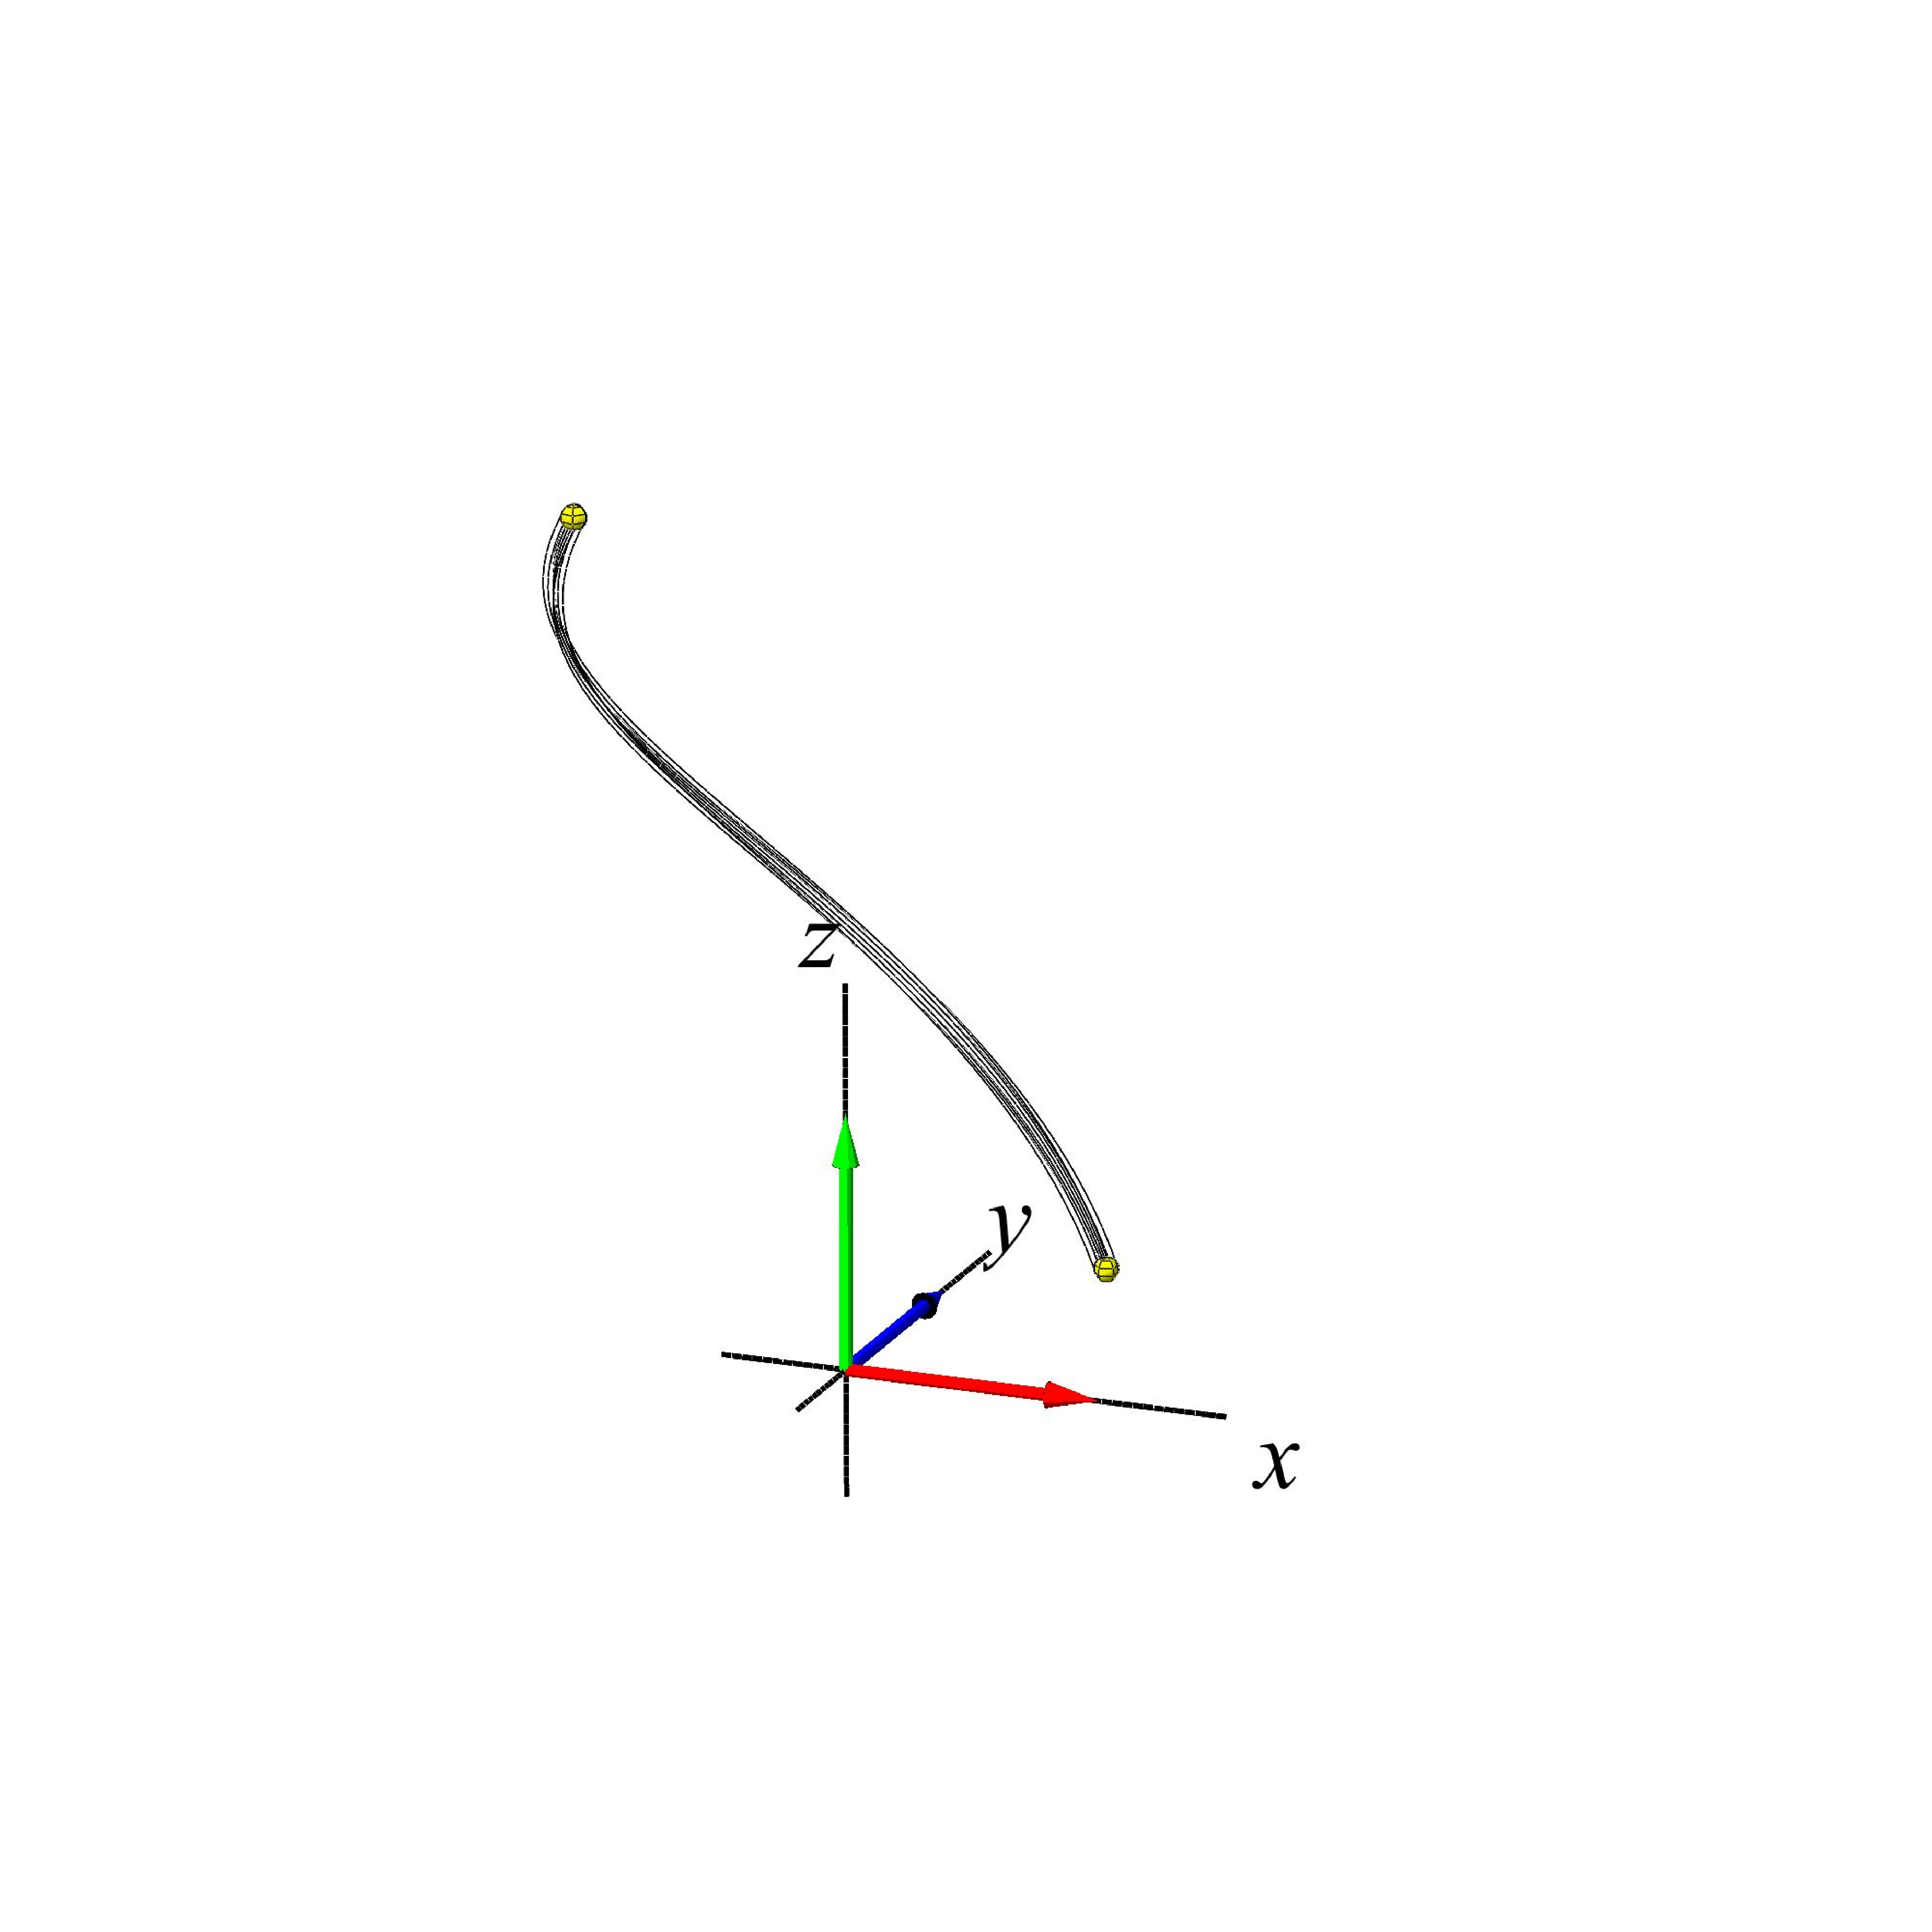
\includegraphics[height=70mm]{FIGS/plotVFrot2}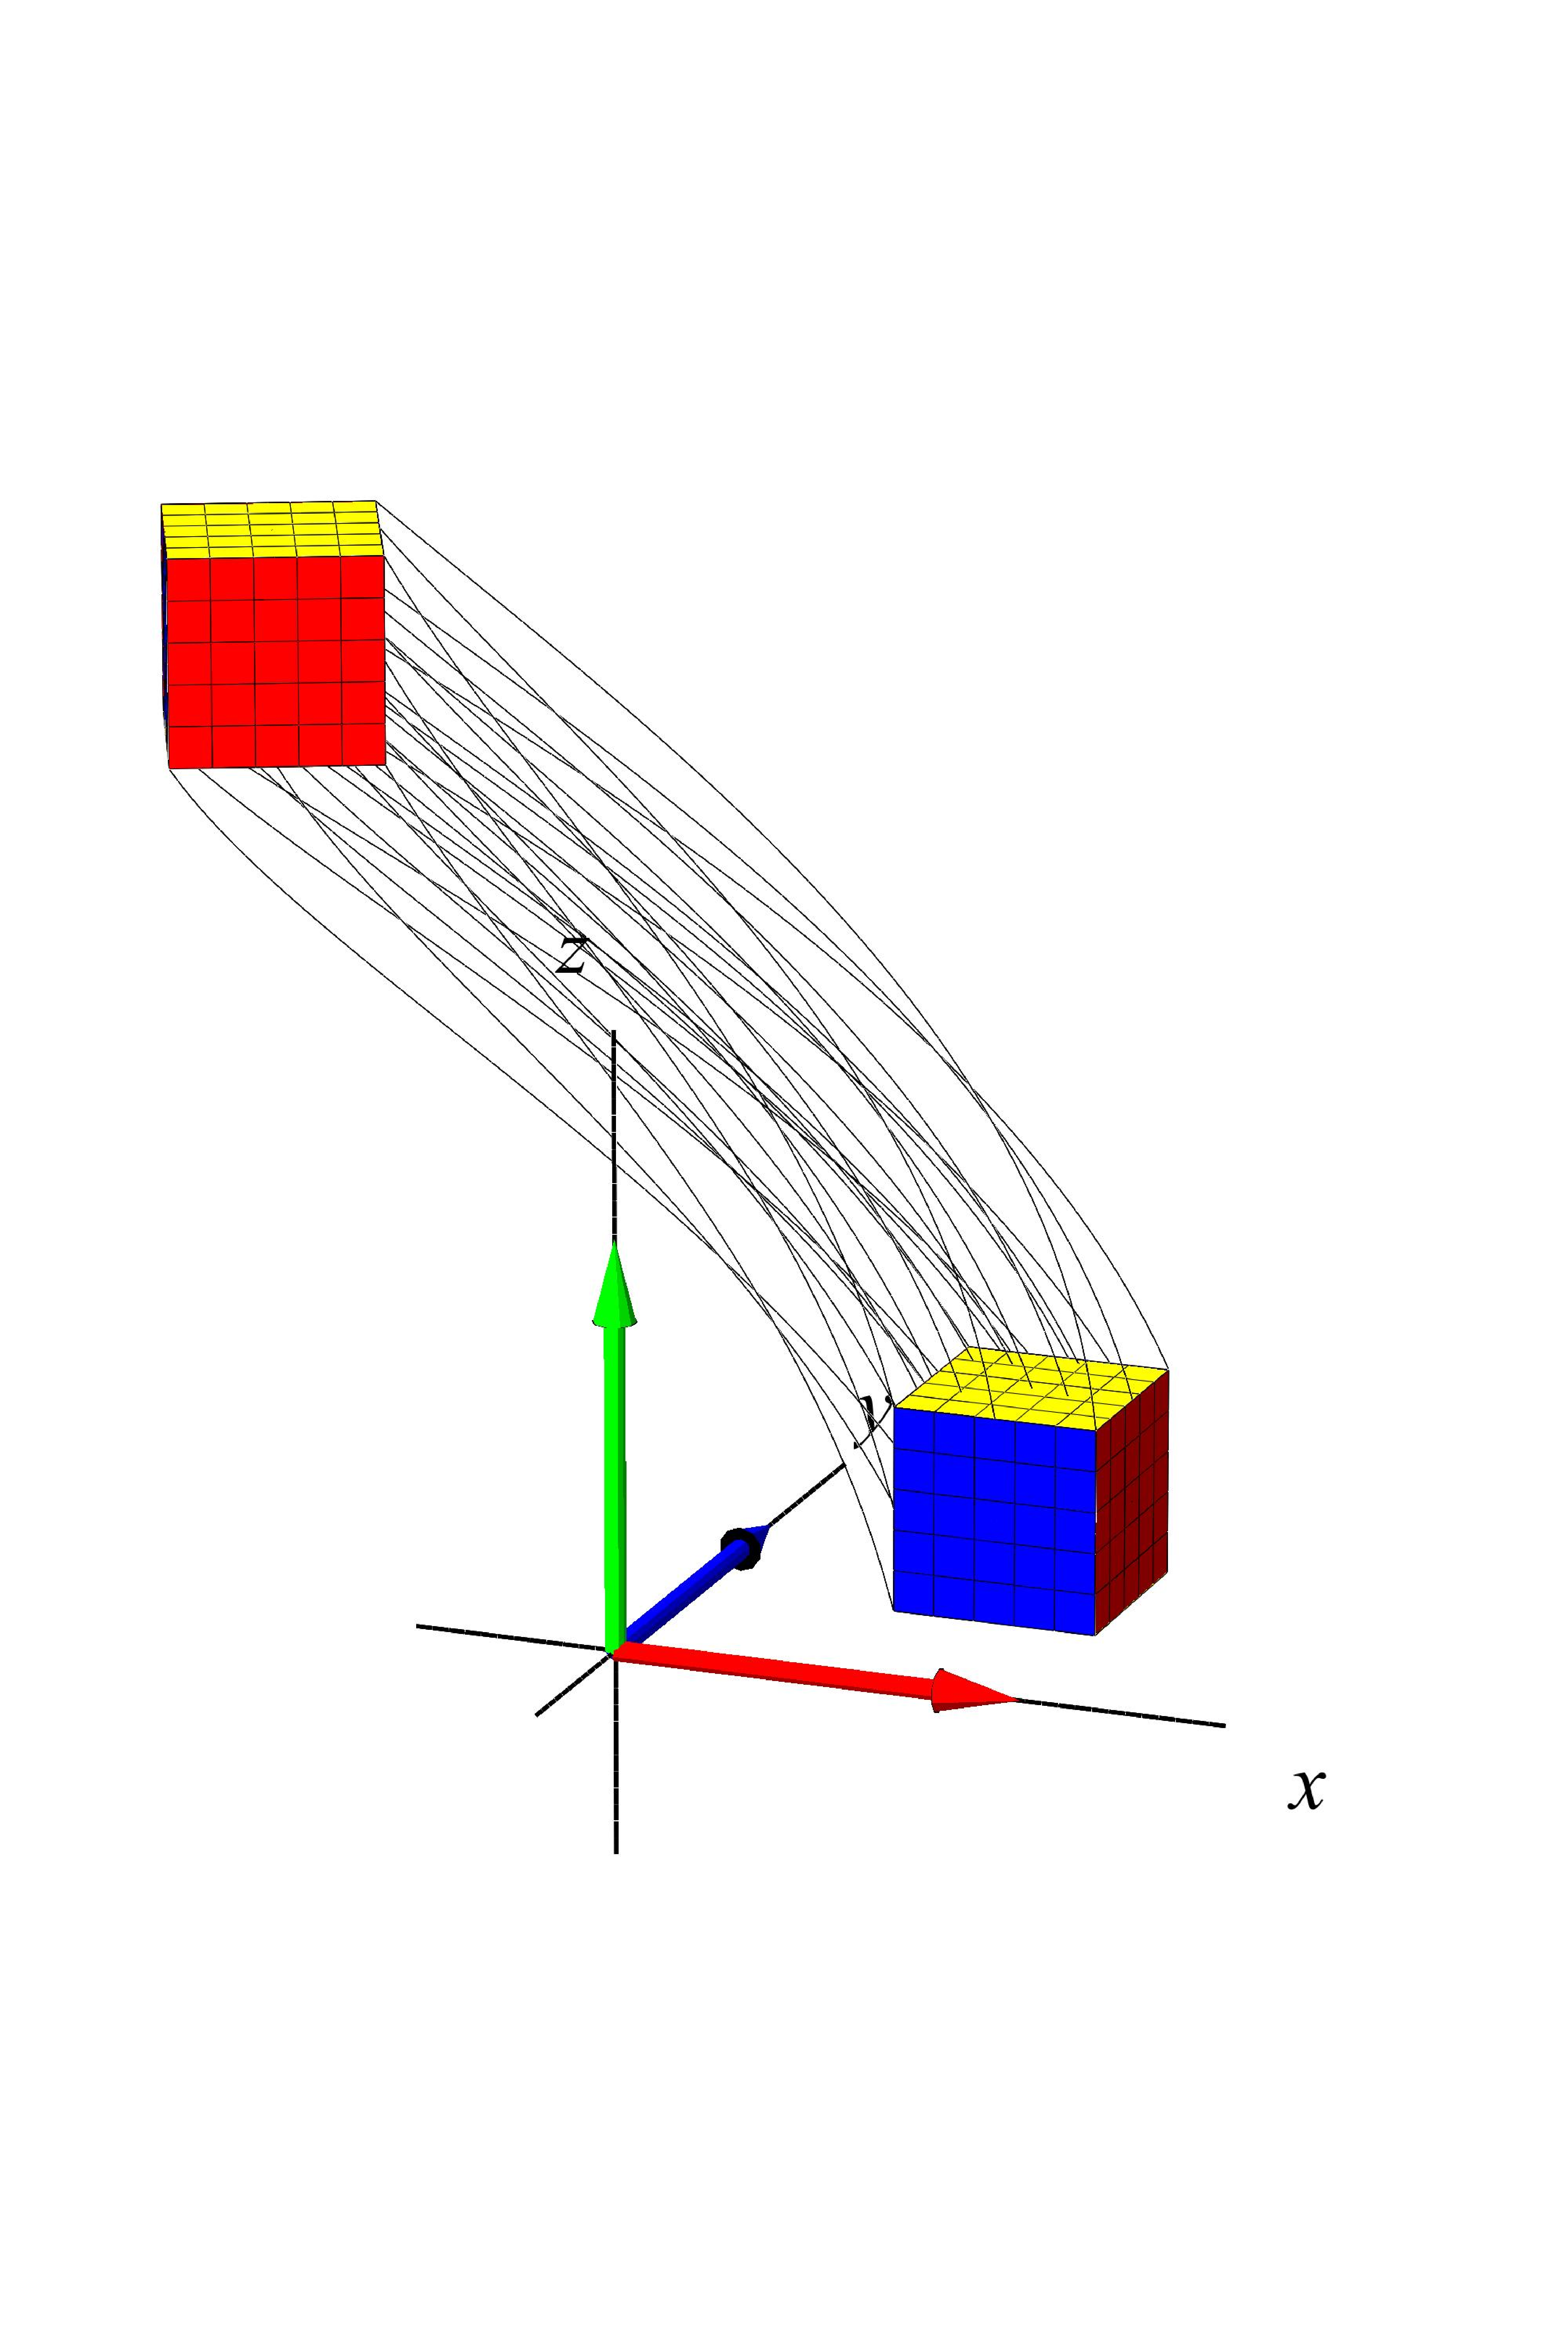
\includegraphics[height=70mm]{FIGS/plotVFrot3}}
\begin{center}
\caption{\small{Det roterende vektorfelt fra
eksempel \ref{exVFrotFlow}, en ''flowkurve'' for en enkelt partikel og  systemet af
flowkurver, som går igennem en terning (den nederste terning flyder langs flowkurverne med vektorfeltet indtil tiden $\pi$.}}
\label{figVFrot}
\end{center}
\end{figure}


\begin{exercise} \label{exerFlowDeform}
Lad $\,{\mathbf{V}}(x,y,z) = (-y, x, 0)\,$ og benyt Maple
til at finde flowkurver og bevægelsen af punkter i samme terning som i figur
\ref{figVFrot} når tidsintervallet for flowet sættes til $\,T = [0,
2\,\pi]\,$. Sammenlign dernæst med 'virkningen' af vektorfelterne
$\,{\mathbf{W}}(x,y,z) = (-y, -x, 0)\,$  $\,{\mathbf{W}}(x,y,z) = (-y, 2\,x, 0)\,$ på terningens punkter i samme
tidsinterval. Forklar forskellene på de tre 'virkninger' af de tre
forskellige vektorfelter på terningen.
\end{exercise}



\begin{example}[Flowkurver for et eksplosions- hhv. implosions-vektorfelt]\label{exVFexplodeFlow}
Eksplosionsvektorfeltet
\begin{equation}
{\mathbf{V}}(x,y,z) = (x, y, z)
\end{equation}
har flowkurver, der tilfredsstiller en begyndelsesbetingelse
\begin{equation}
(x(0), y(0), z(0)) = (x_{0},
y_{0}, z_{0})
\end{equation}
og differentialligningerne
\begin{equation}
{\mathbf{r}}'(t) = (x'(t),
y'(t), z'(t)) = (x(t), y(t), z(t)) \quad .
\end{equation}
Vi  finder de tre koordinatfunktioner  $x(t)$, $y(t)$, og $z(t)$ sådan at
\begin{equation}
\begin{aligned}
x'(t) &= x(t) \\
y'(t) &=  y(t) \\
z'(t) &=  z(t) \quad .
\end{aligned}
\end{equation}
 Differentialligningerne
for $x(t)$, $y(t)$, og $z(t)$ er her u-koblede lineære
differentialligninger, som let løses en af gangen. Resultatet er
\begin{equation}
x(t) = x_{0}\exp(t)\quad , \qquad
y(t) = y_{0}\exp(t)\quad , \quad \textrm{og}
\quad z(t) = z_{0}\exp(t) \quad .
\end{equation}
 Bemærk, at
hvis $(x(0), y(0), z(0)) = (0,0,0)$ så er $(x(t),
y(t), z(t)) = (0,0,0)$ for alle $\, t \in
[-\infty, \infty] \,$. Flowkurven 'igennem'
punktet $\,(0,0,0)\,$ er derfor ikke nogen
egentlig 'kurve' men består 'kun' af punktet
selv. Bemærk også, at alle andre flowkurver
kommer vilkårligt tæt på punktet $(0,0,0)$ for $t
\to -\infty$, idet $\,\exp(t) \to 0$ for $t \to
-\infty\,$, men de går ikke igennem punktet. Hvis
vi følger flowkurverne i figur \ref{figVFexplode}
tilbage i tid fra $t = 0$ igennem negative
værdier vil vi derfor se en eksponentielt
aftagende {\em{{implosion}}} af terningen. Hvis vi
derimod følger flowkurverne frem i tid fra $t =
0$ igennem større og større positive værdier for
$t$ vil vi se en eksponentielt voksende
eks\-plo\-sion af terningen. Flowkurverne kan
igen findes og inspiceres med
Maple. Se figur
\ref{figVFexplode}.\\

Implosionsvektorfeltet er givet ved
\begin{equation}
{\mathbf{V}}(x,y,z) = (-x, -y, -z)
\end{equation}
med de ''tids-omvendte'' løsninger (i forhold til eksplosionsvektorfeltet)
\begin{equation}
x(t) = x_{0}\exp(-t)\quad , \qquad
y(t) = y_{0}\exp(-t)\quad , \quad \textrm{og}
\quad z(t) = z_{0}\exp(-t) \quad .
\end{equation}
Se figur \ref{figVFimplode}.
\end{example}



\begin{figure}[h]
\centerline{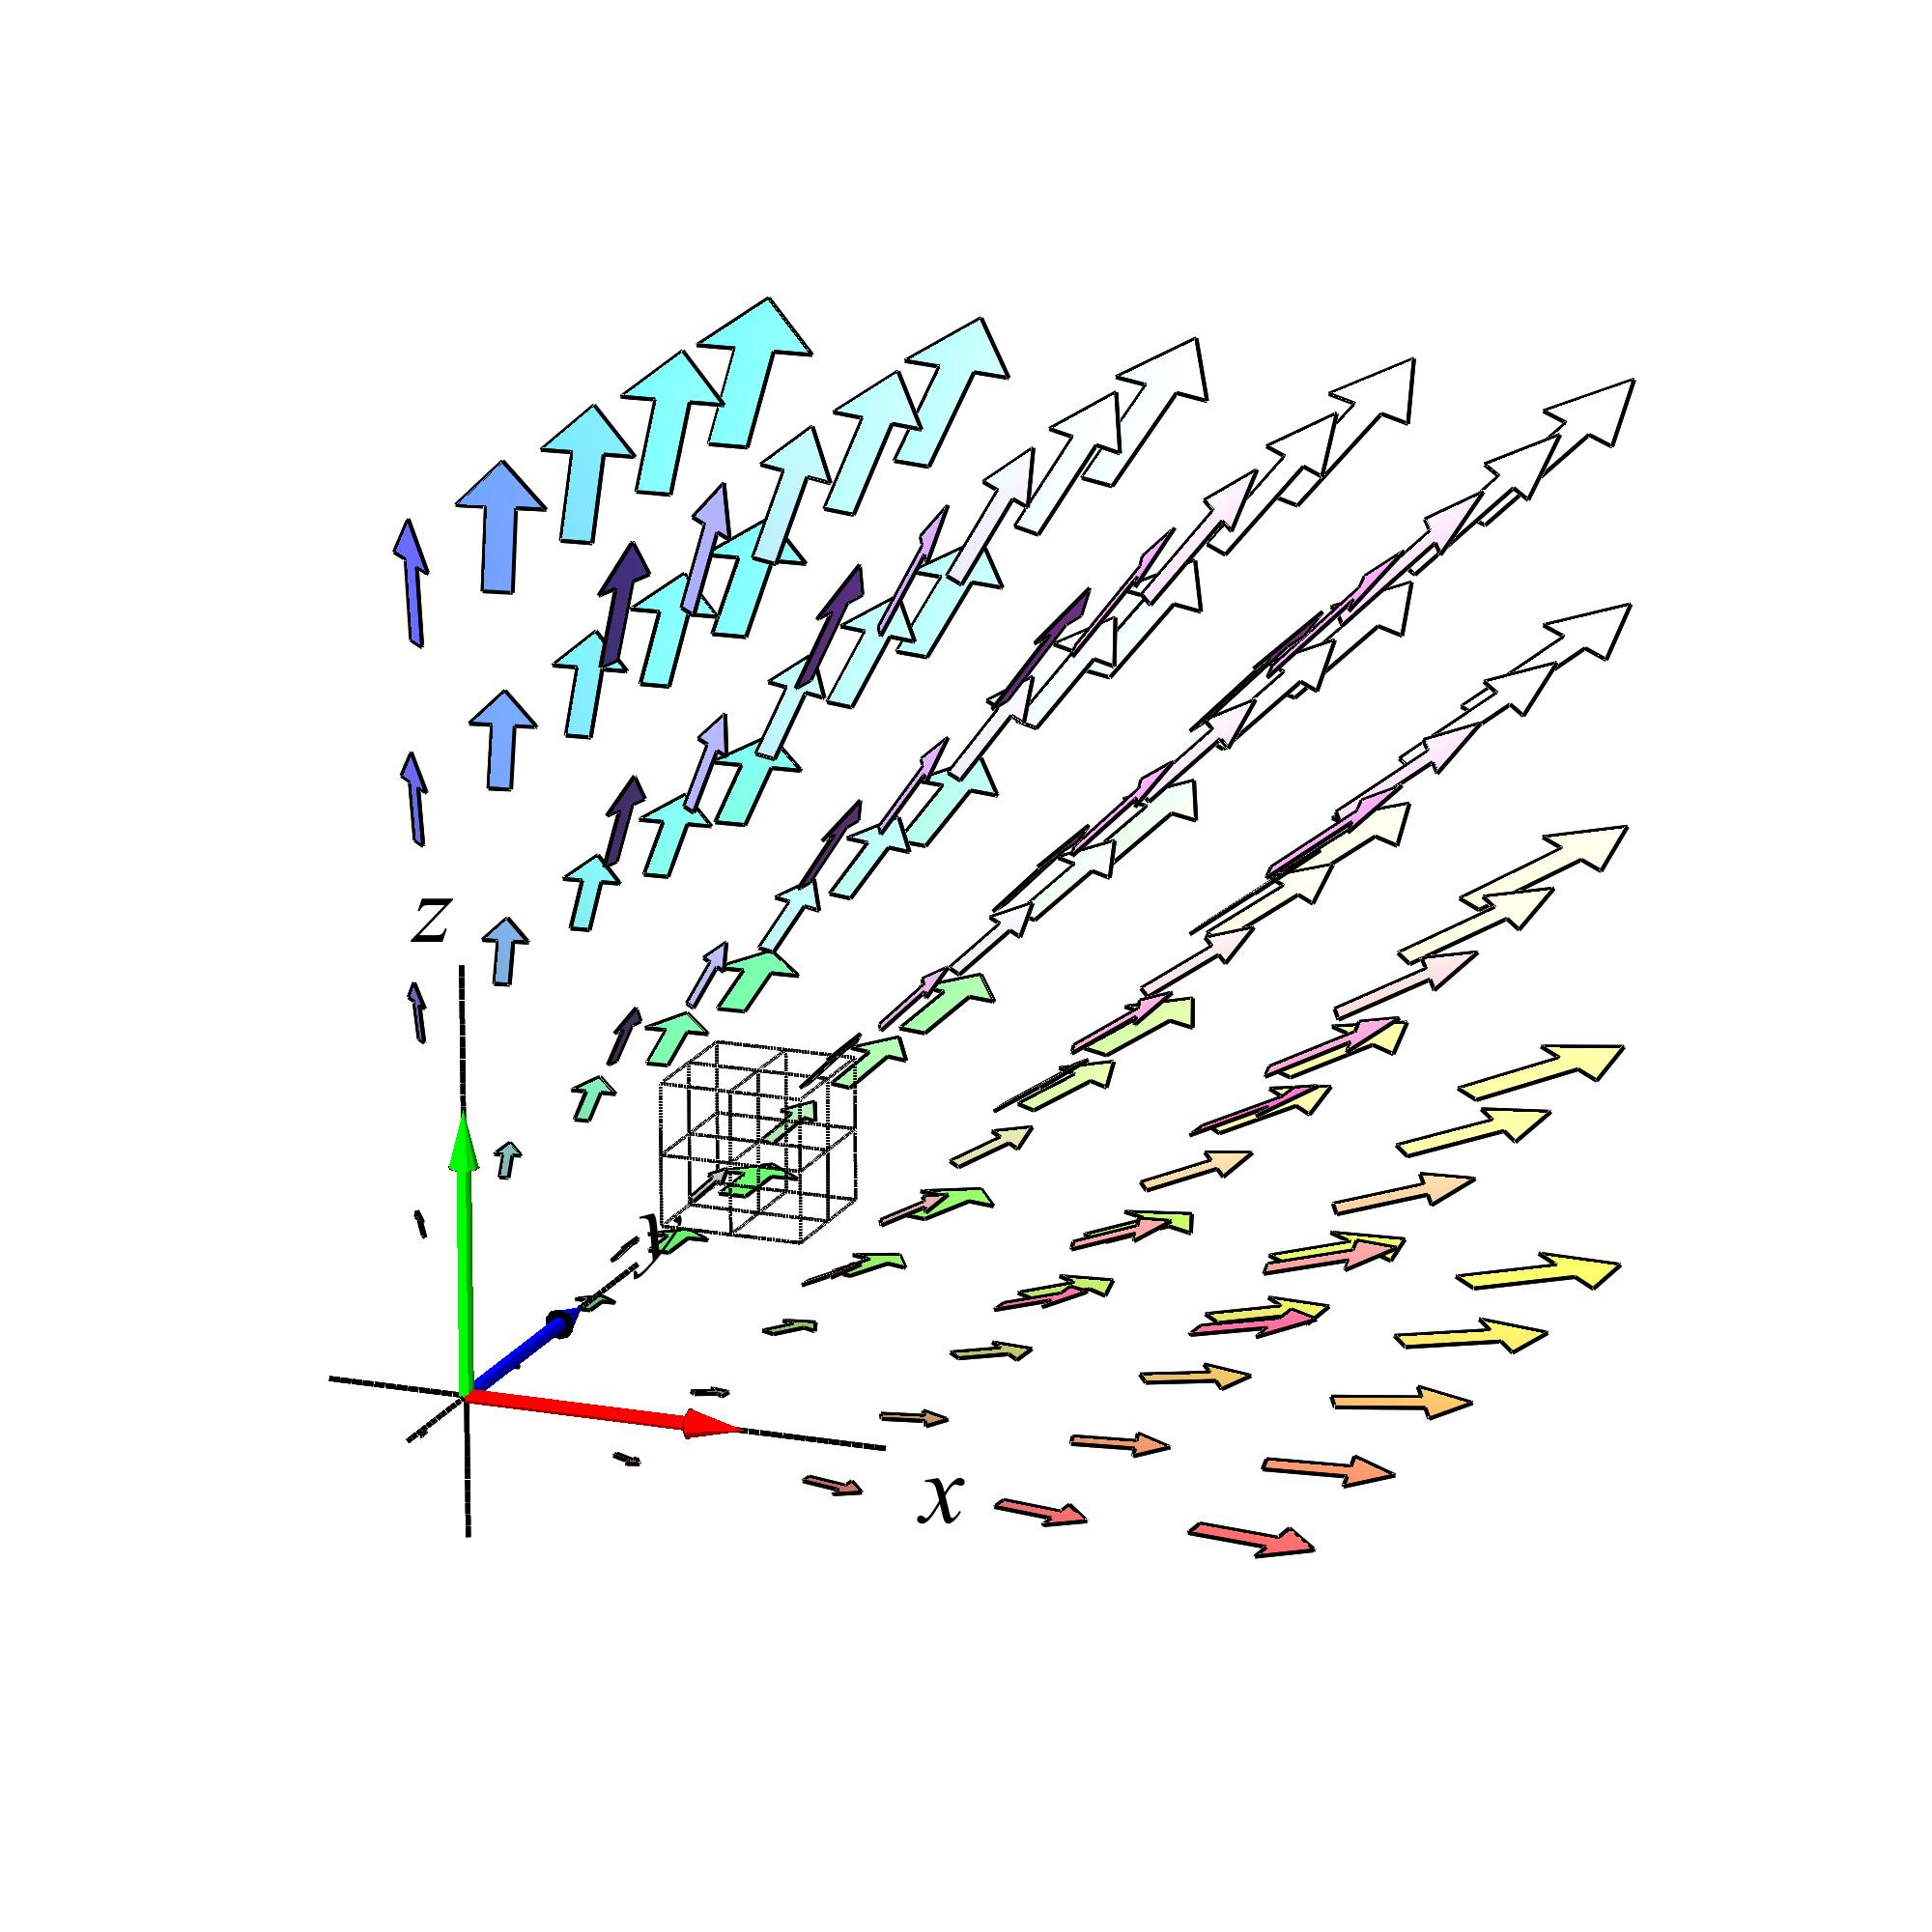
\includegraphics[height=70mm]{FIGS/plotVFexplode1}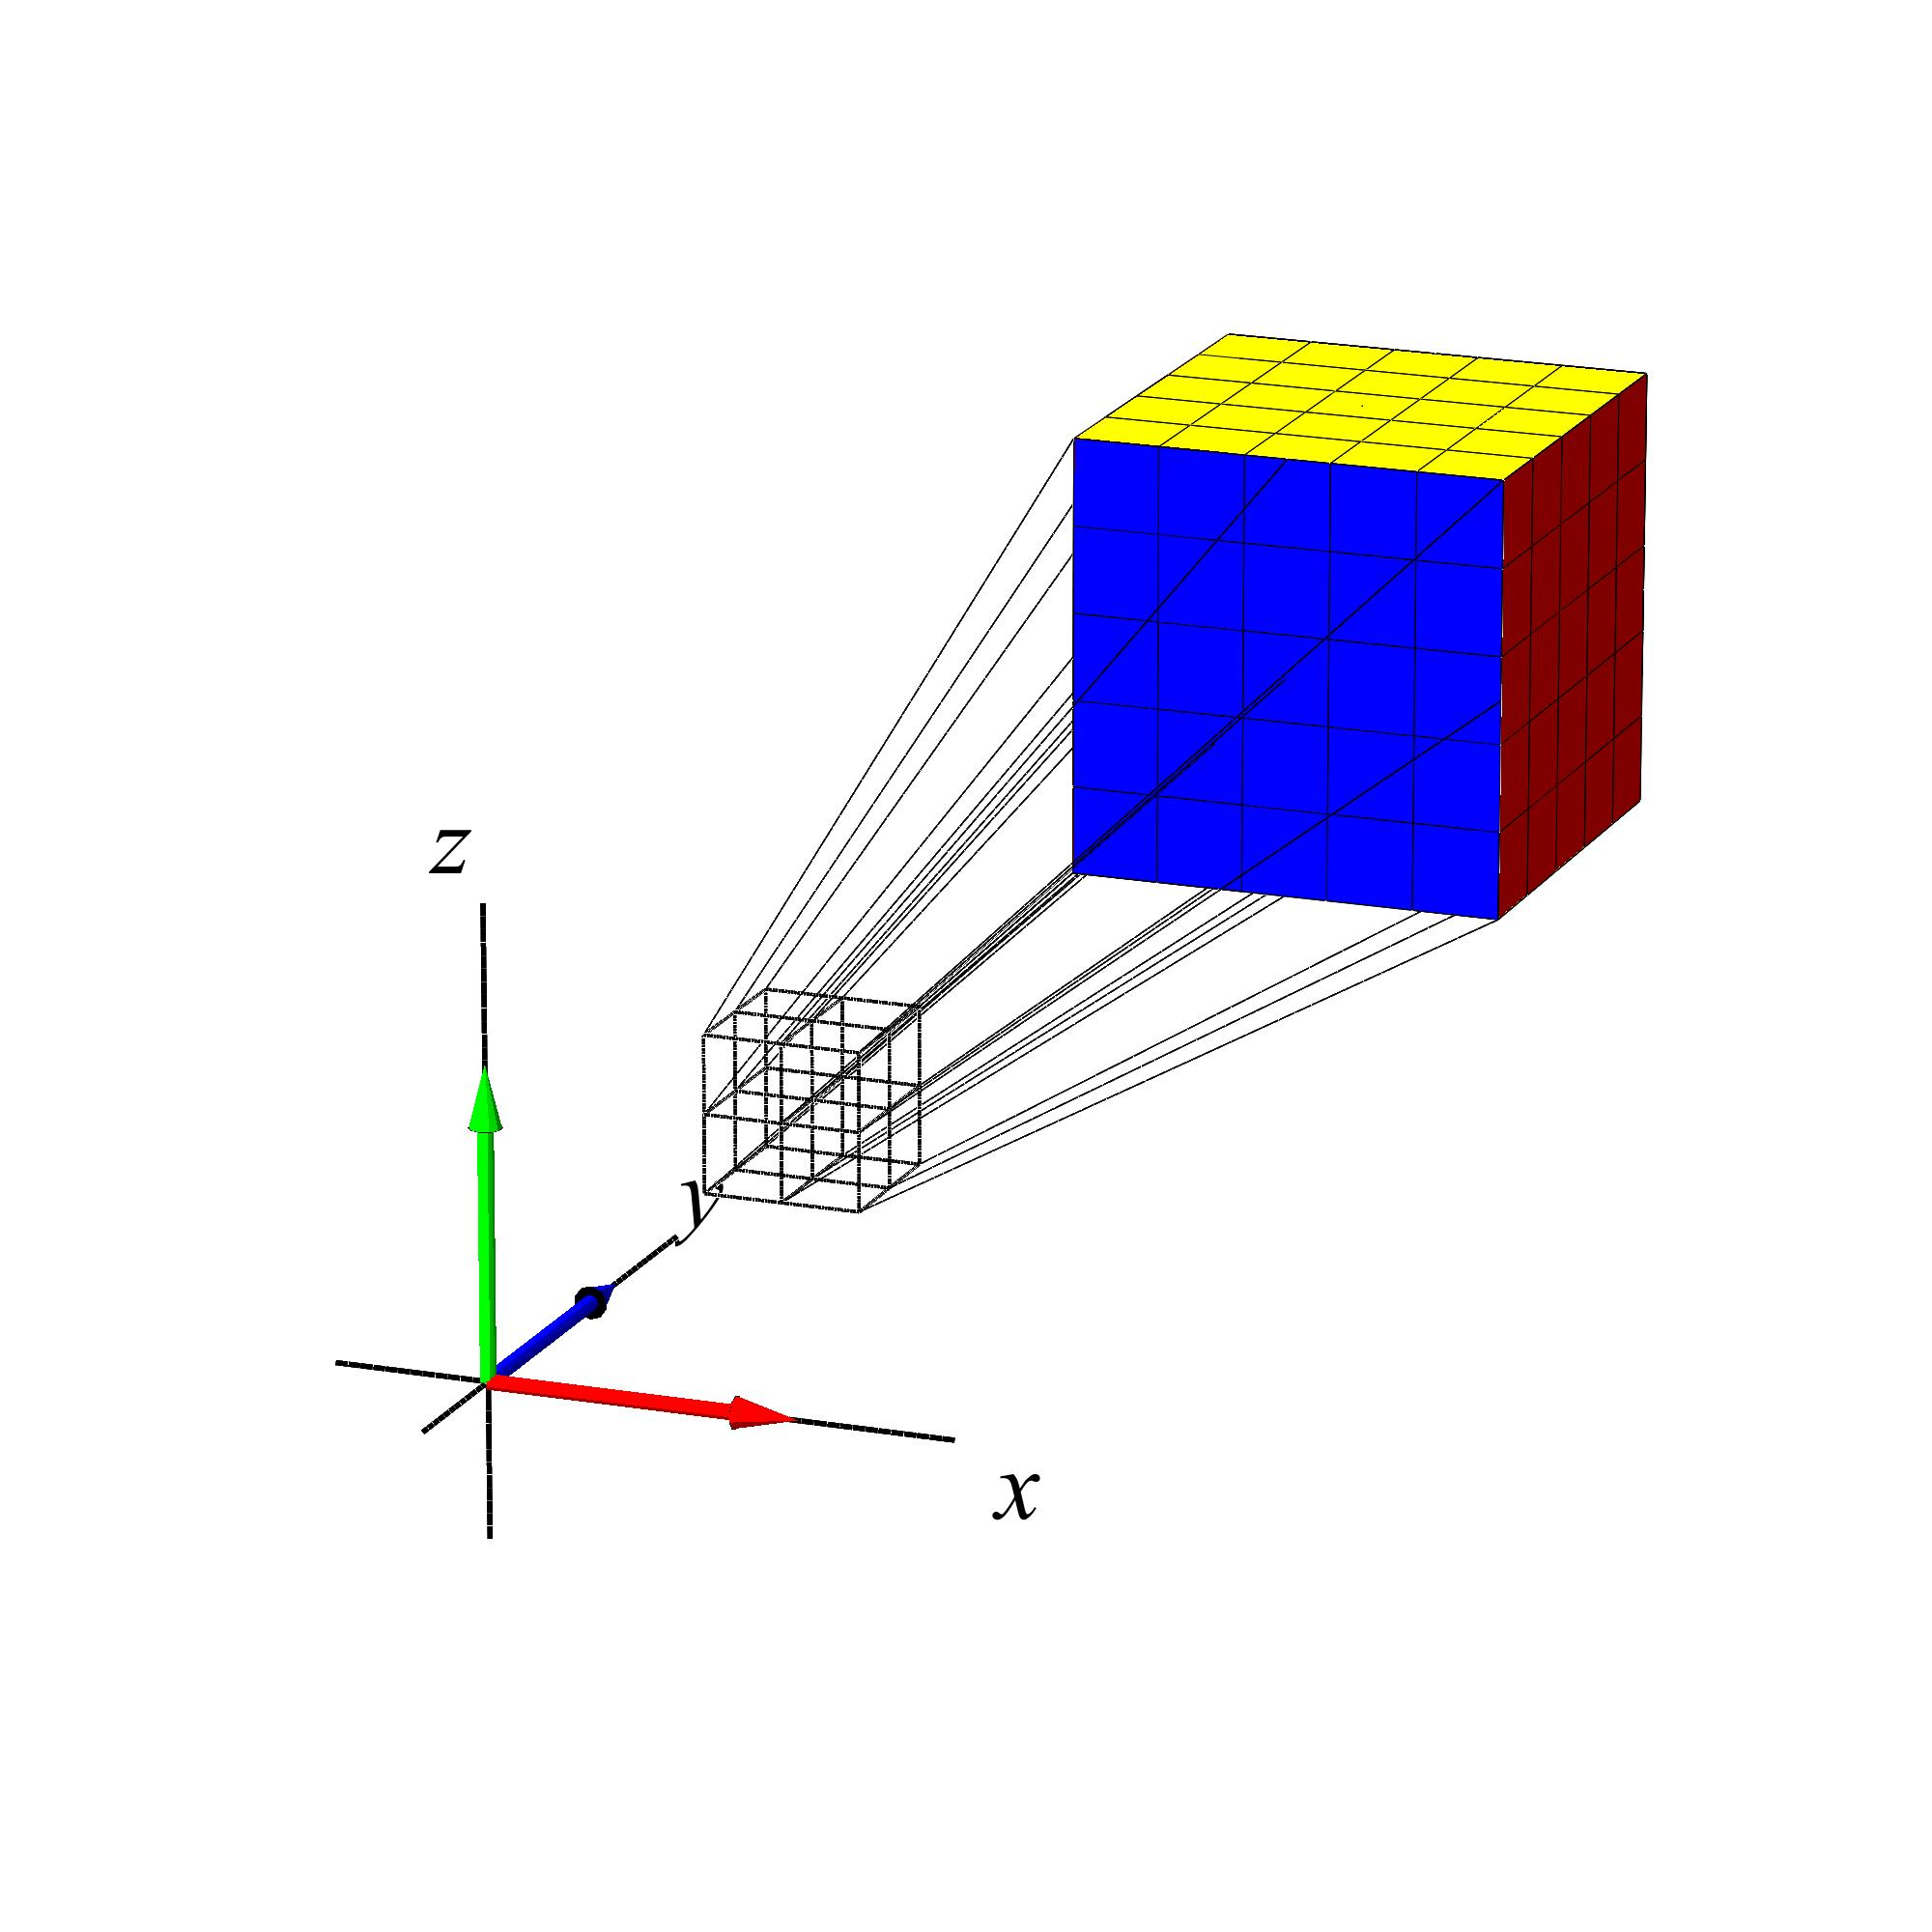
\includegraphics[height=70mm]{FIGS/plotVFexplode2}}
\begin{center}
\caption{\small{Eksplosionsvektorfeltet fra
eksempel \ref{exVFexplodeFlow} sammen med de
integralkurver, som går igennem en terning. Terningen er vist solid til tiden $t=1$ og ''åben'' til tiden $t=0$. Sammenlign med figur \ref{figVFimplode}.}}
\label{figVFexplode}
\end{center}
\end{figure}


\begin{figure}[h]
\centerline{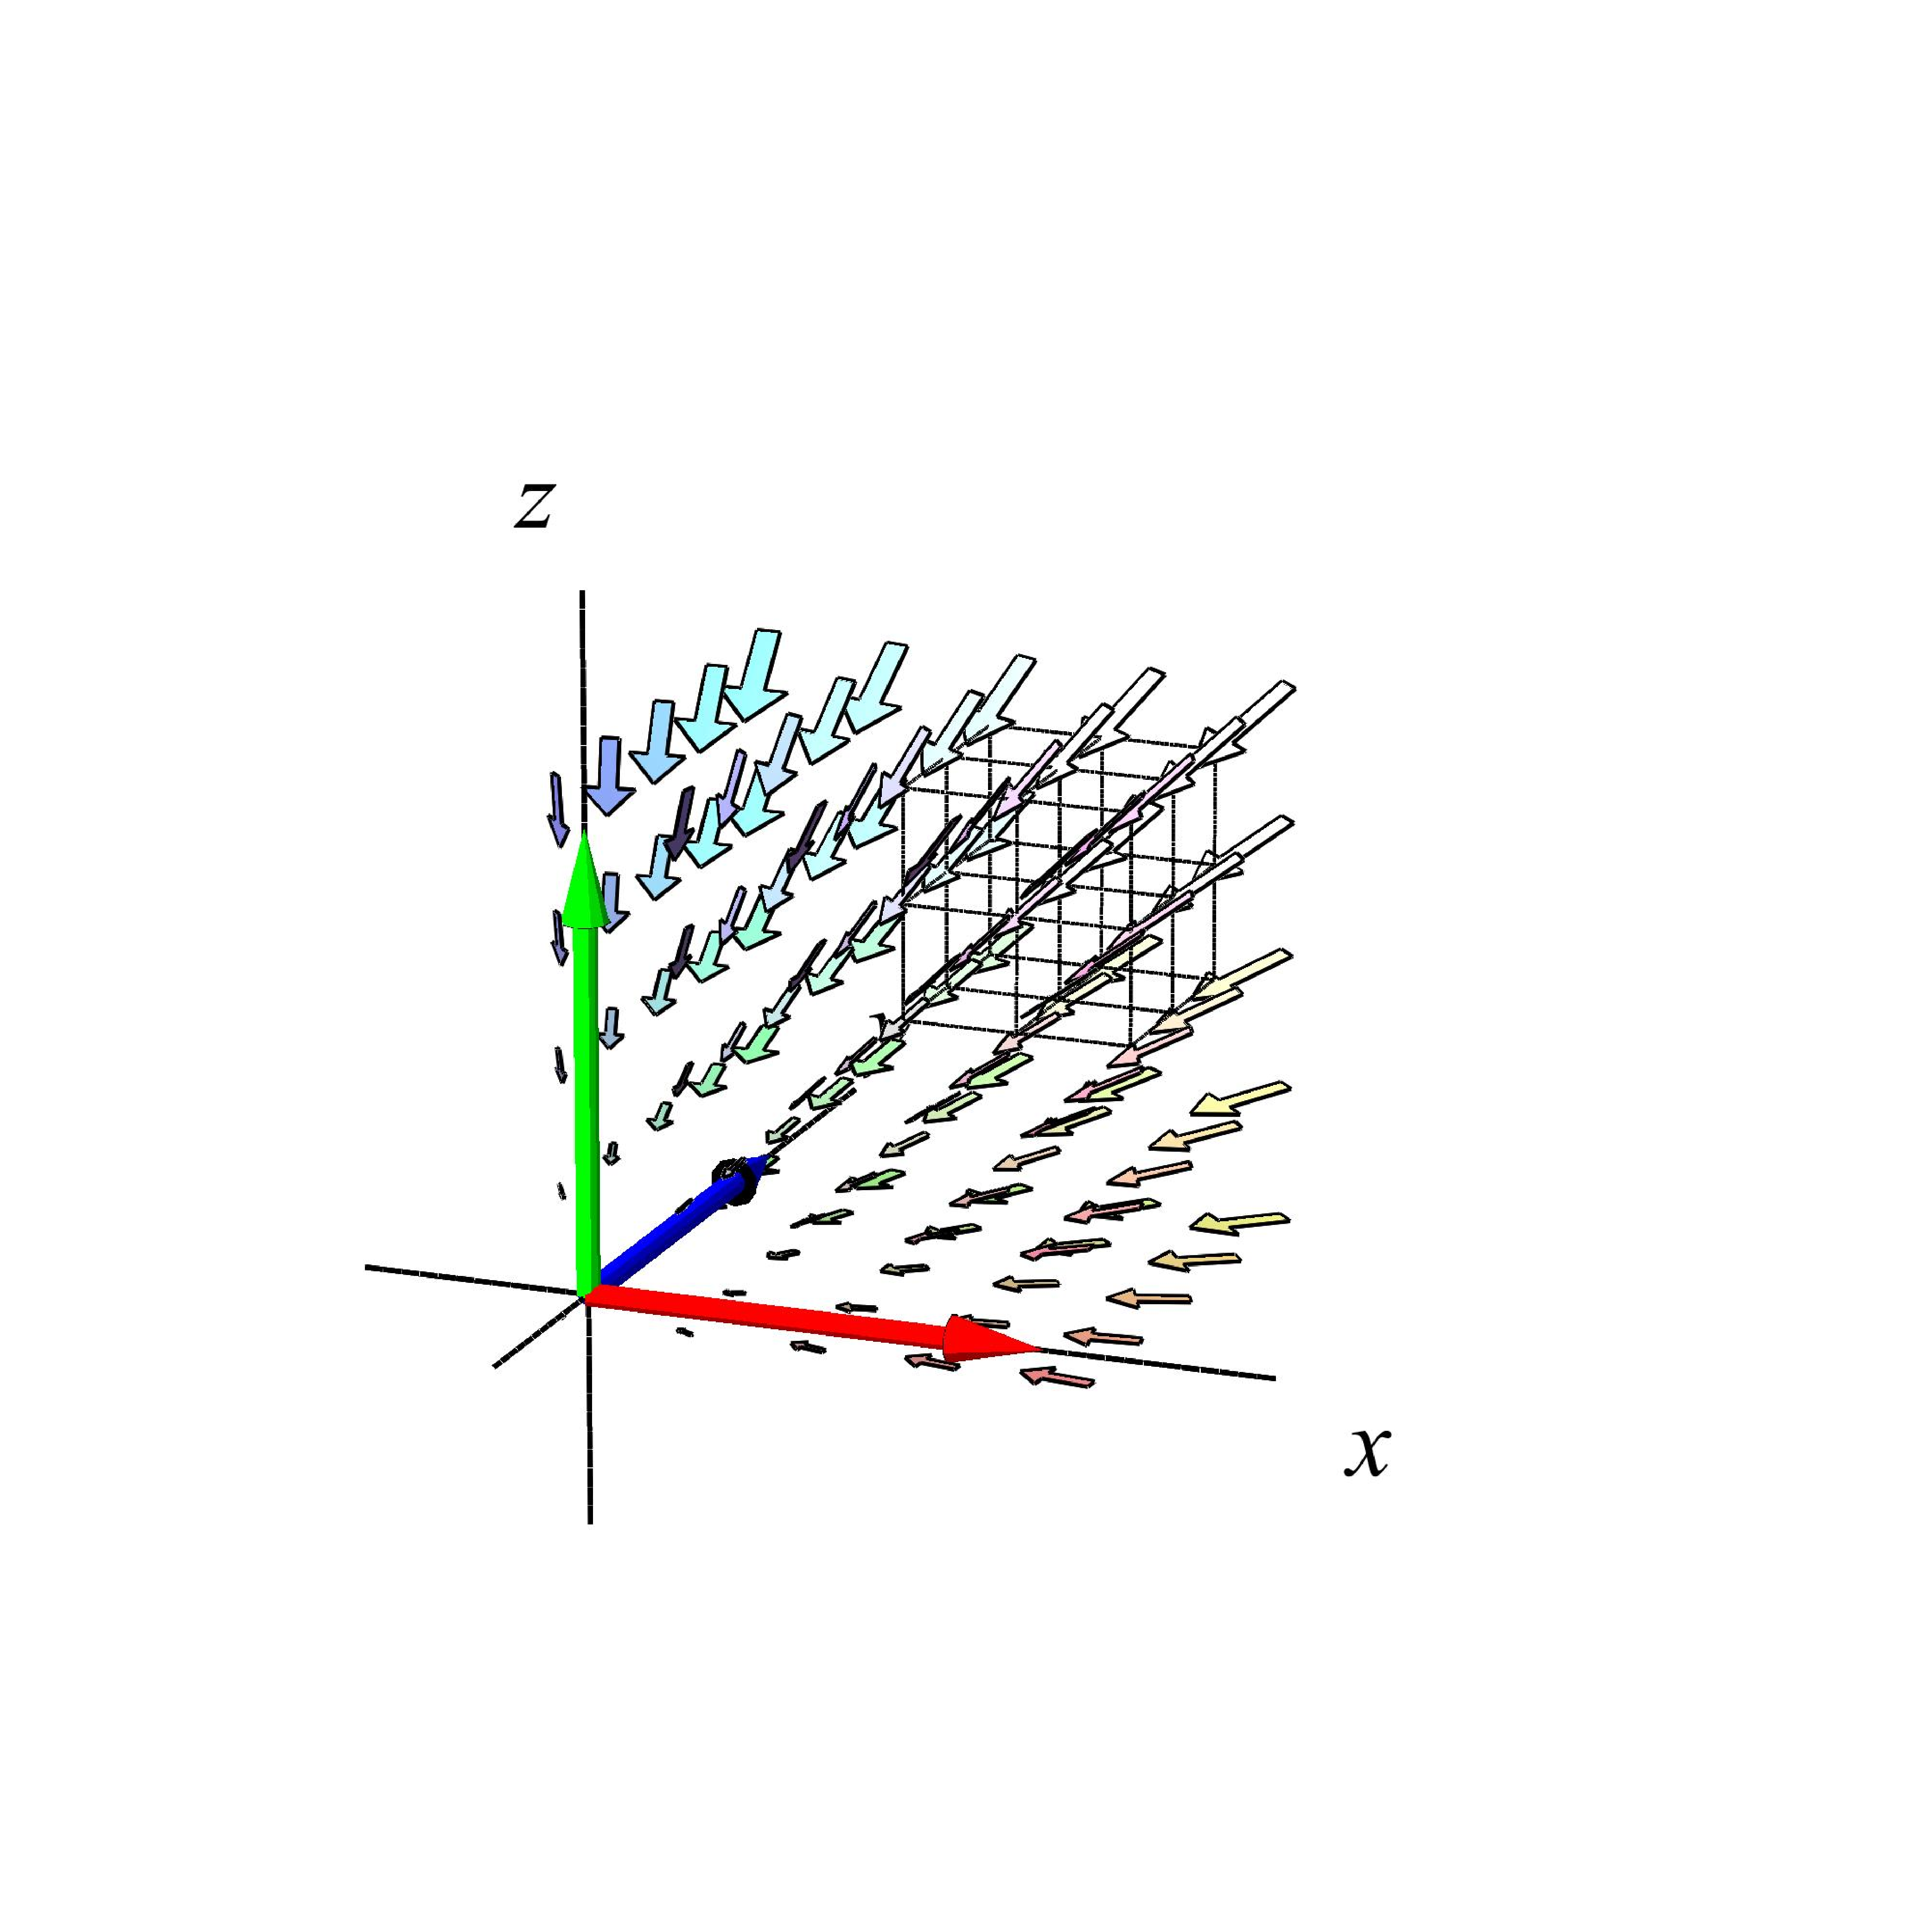
\includegraphics[height=70mm]{FIGS/plotVFimplode1}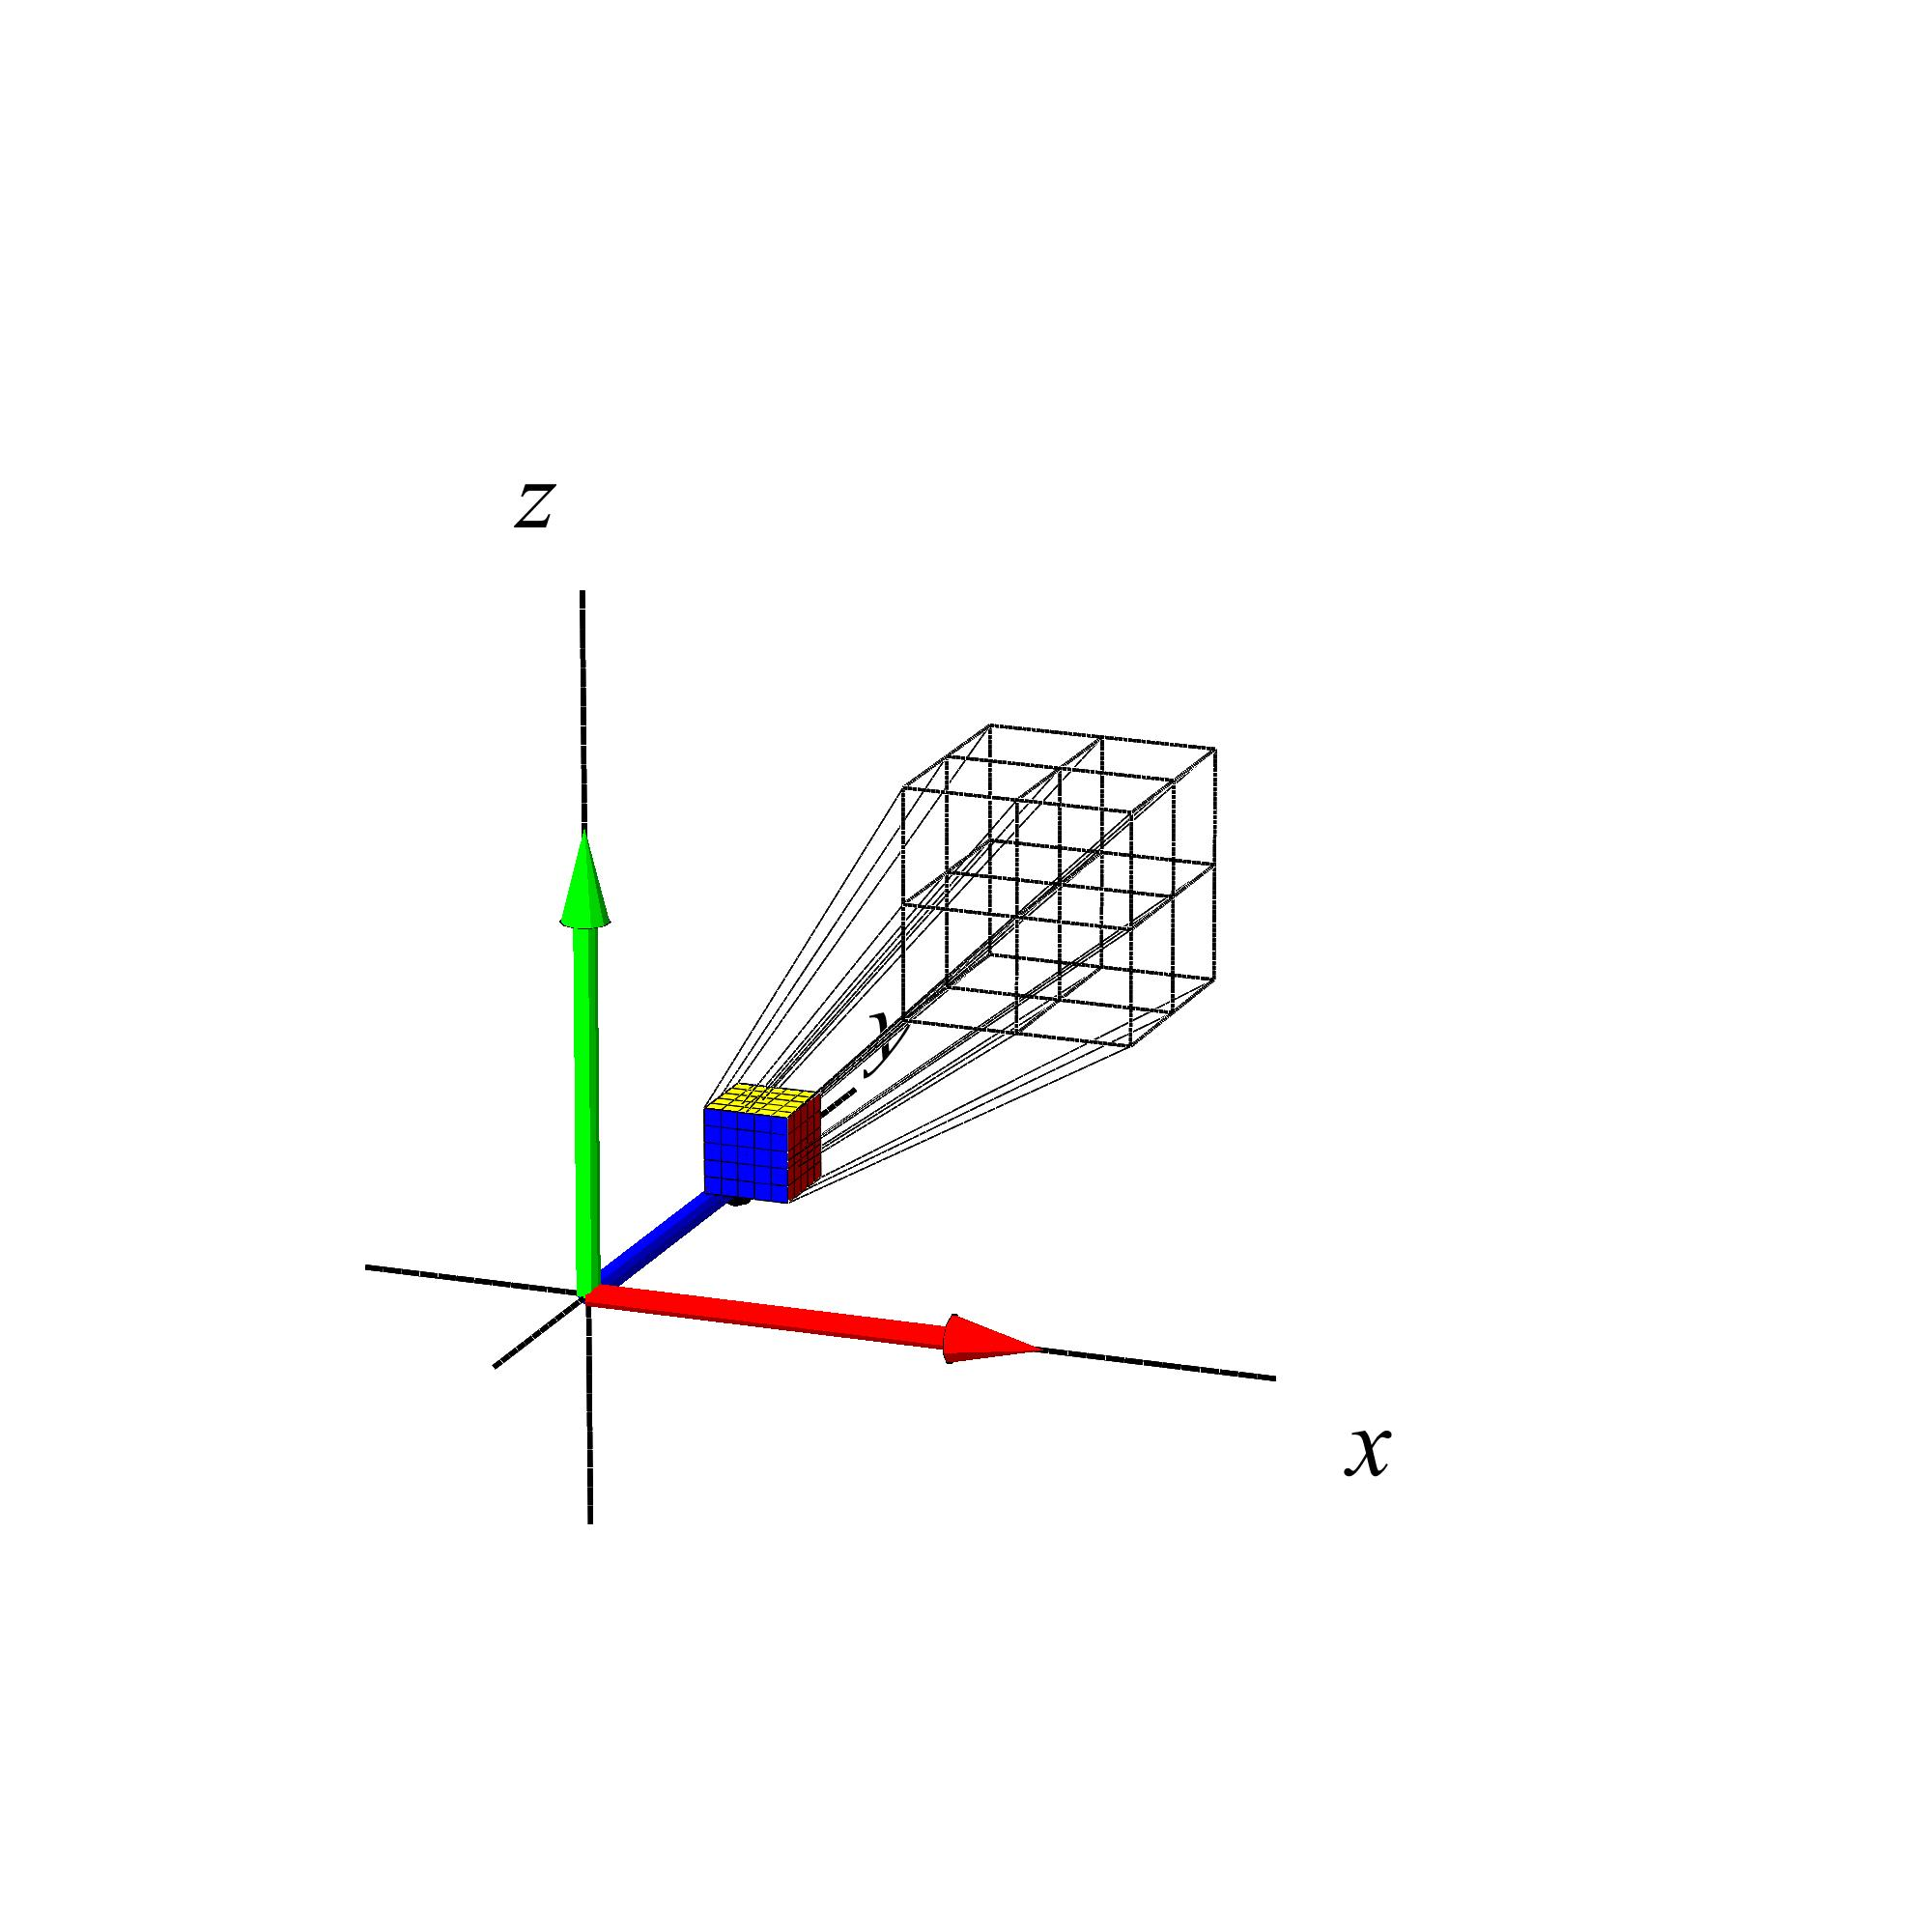
\includegraphics[height=70mm]{FIGS/plotVFimplode2}}
\begin{center}
\caption{\small{Implosionsvektorfeltet fra
eksempel \ref{exVFexplodeFlow} sammen med de
integralkurver, som går igennem en terning.  Terningen er vist solid til tiden $t=1$ og ''åben'' til tiden $t=0$. Sammenlign med figur \ref{figVFexplode}.}}
\label{figVFimplode}
\end{center}
\end{figure}




\begin{exercise}
Lad ${\mathbf{V}}$ betegne vektorfeltet $\,
{\mathbf{V}}(x,y,z) = (-x, -2y, -3z)\, $. Find og vis
 et passende antal af
flowkurverne for vektorfeltet igennem den kugle
der har centrum i $(1,0,0)$ og radius
$\frac{1}{4}$.
\end{exercise}





%%%%%%%%%%%%%%%%%%%%%%%%%%%%%%%%%%%%%%%%%%%%%%%%%%%
%%%%%%%%%%%%%%%%%%%%%%%%%%%%%%%%%%%%%%%%%%%%%%%%%%%
%%%%%%%%%%%%%%%%%%%%%%%%%%%%%%%%%%%%%%%%%%%%%%%%%%%
%%%%%%%%%%%%%%%%%%%%%%%%%%%%%%%%%%%%%%%%%%%%%%%%%%%







\section{Divergensen af et vektorfelt} \label{secDiv}

Med henblik på den geometriske analyse af vektorfelter og deres flowkurve-egenskaber vil vi her indføre to værktøjer, to begreber,  til
lokal beskrivelse af generelle glatte vektorfelter. Beskrivelsen er lokal fordi begge begreberne er udtrykt ved de partielle afledede af vektorfeltets koordinatfunktioner.

\begin{definition}
Lad ${\mathbf{V}}(x,y,z) \,= \, (V_{1}(x,y,z), \, V_{2}(x,y,z), \,
V_{3}(x,y,z) \,)\,$ være et vektorfelt i rummet. {\em{{Divergensen}}}
af $\,{\mathbf{V}}\,$ i punktet $\,(x_{0},y_{0},z_{0})\,$ defineres
således:
\begin{equation}
\operatorname{Div}({\mathbf{V}})(x_{0},y_{0},z_{0}) \, = \,
\frac{\partial V_{1}}{\partial
x}(x_{0},y_{0},z_{0}) + \frac{\partial
V_{2}}{\partial y}(x_{0},y_{0},z_{0}) +
\frac{\partial V_{3}}{\partial
z}(x_{0},y_{0},z_{0}) \quad .
\end{equation}
Hvis ${\mathbf{V}}(x,y) \,= \, (V_{1}(x,y), \, V_{2}(x,y)\,)\,$  er et \emph{plant vektorfelt} definerer vi helt tilsvarende:
\begin{equation}
\operatorname{Div}({\mathbf{V}})(x_{0},y_{0}) \, = \,
\frac{\partial V_{1}}{\partial
x}(x_{0},y_{0}) + \frac{\partial
V_{2}}{\partial y}(x_{0},y_{0}) \quad .
\end{equation}
\end{definition}

\begin{think}
Divergensen af et glat vektorfelt i $\mathbf{R}^{3}$ er en glat \emph{funktion} i $\mathbf{R}^{3}$.
\end{think}

\begin{aha}
Læg mærke til, at divergensen af et plant vektorfelt er det samme som divergensen af feltets rumlige udvidelse.
\end{aha}


\begin{example}[Simple divergenser] \label{exampDivExplode}
Ethvert konstant vektorfelt ${\mathbf{V}}(x,y,z) = \mathbf{b}$ har
divergens $\,\operatorname{Div}({\mathbf{V}}) = 0\,$. \\

Eksplosionsvektorfeltet ${\mathbf{V}}(x,y,z) = (x, y, z)$ har konstant
divergens $\,\operatorname{Div}({\mathbf{V}}) = 3\,$. \\

Implosionsvektorfeltet ${\mathbf{V}}(x,y,z) = (-x, -y, -z)$ har divergensen
 $\,\operatorname{Div}({\mathbf{V}}) = -3\,$. \\

 Det roterende vektorfelt
$\,{\mathbf{V}}(x,y,z) = (-y, x, 0)$ har også konstant divergens:
$\,\operatorname{Div}({\mathbf{V}}) = 0\,$.
\end{example}


\begin{exercise}
Lad ${\mathbf{V}}(x,y,z) = (x + \sin(y),\, z + \cos(y),\, x+y-z)$.
Bestem $\,\operatorname{Div}({\mathbf{V}})\,$ i ethvert punkt i rummet.
\end{exercise}

\begin{exercise}
Lad ${\mathbf{V}}(x,y,z)$ være et vektorfelt af
  første grad med matrix-fremstilling som i
ligning (\ref{eqVFmatrix}). Vis, at divergensen
af ${\mathbf{V}}(x,y,z)$ er konstant lig med sporet
af ${\mathbf{A}}$.
\end{exercise}



\begin{exercise}
Lad ${\mathbf{V}}(x,y,z) = {\bm{\nabla}}h(x,y,z)$ være gradientvektorfeltet
for en given funktion $\,h(x,y,z)\,$. Vis, at divergensen af
${\mathbf{V}}(x,y,z)$ er
\begin{equation}
\operatorname{Div}({\bm{\nabla}}h(x,y,z)) = \frac{\partial^{2}\,h}{\partial\,x^{2}} +
\frac{\partial^{2}\,h}{\partial\,y^{2}} +
\frac{\partial^{2}\,h}{\partial\,z^{2}} \quad .
\end{equation}
\end{exercise}

 I anvendelserne af vektoranalysen benyttes meget ofte divergensen af gradienvektorfelter for givne funktioner, $\operatorname{Div}({\bm{\nabla}}h(x,y,z))$, som derfor
gives sin egen betegnelse:

\begin{definition}
Lad $h(x,y,z)$ betegne en glat funktion i $\mathbb{R}^{3}$. Så skriver vi:
\begin{equation}
\begin{aligned}
\Delta h(x,y,z) &= \operatorname{Div}({\bm{\nabla}}h(x,y,z)) \\
 &= \frac{\partial^{2}\,h}{\partial\,x^{2}} +
\frac{\partial^{2}\,h}{\partial\,y^{2}} +
\frac{\partial^{2}\,h}{\partial\,z^{2}} \quad .
\end{aligned}
\end{equation}
Funktionen $\Delta h(x,y,z)$ kaldes {\emph{den Laplace-afledede}} af funktionen $h(x,y,z)$.
\end{definition}

\begin{example}[Laplace afledede]\label{exampLaplacians}
Laplace-afledede af nogle elementære funktioner af tre variable:
\begin{equation}
\begin{array}{|l|c|c|}
  \hline
  % after \\: \hline or \cline{col1-col2} \cline{col3-col4} ...
 \textrm{Funktion} & \bm{\nabla}f(x,y,z) & \Delta f(x,y,z) \\ \hline \hline
 f(x,y,z)= a\cdot x+b\cdot y+c\cdot z & (a,b,c)   & 0             \\ \hline
 f(x,y,z)= x^{2} + y^{2} + z^{2} & (2x, 2y, 2z) & 6                \\ \hline
  f(x,y,z)= y\cdot \sin(x) & (y\cdot \cos(x), \sin(x), \, 0) & -y\cdot \sin(x)                \\ \hline
   f(x,y,z)= \e^{x}\cdot \cos(z) & (\e^{x} \cdot \cos(z), \, 0 \, , -\e^{x} \cdot \sin(z))&        0     \\ \hline
 \hline
\end{array}
\end{equation}
\end{example}

\begin{aha}
Den Laplace afledede af en glat funktion $f(x,y,z)$ er sporet af $3 \times 3$-Hesse-matricen for $f$ (se \tref{NUID33-tn18}{eNote}):
\begin{equation}
\Delta f(x,y,z) = \textbf{spor}(\bm{H}f(x,y,z)) \quad .
\end{equation}
\end{aha}


%%%%%%%%%%%%%%%%%%%%%%%%%%%%%%%%%%%%%%%%%%%%%%%%%%%
%%%%%%%%%%%%%%%%%%%%%%%%%%%%%%%%%%%%%%%%%%%%%%%%%%%
%%%%%%%%%%%%%%%%%%%%%%%%%%%%%%%%%%%%%%%%%%%%%%%%%%%
%%%%%%%%%%%%%%%%%%%%%%%%%%%%%%%%%%%%%%%%%%%%%%%%%%%




\section{Rotationen af et vektorfelt} \label{secRot}

Det andet helt centrale begreb og værktøj til analyse af vektorfelter er følgende:

\begin{definition}[Rotation af vektorfelt] \label{defRot}
Lad ${\mathbf{V}}(x,y,z)\,= \, (V_{1}(x,y,z), \, V_{2}(x,y,z), \,
V_{3}(x,y,z) \,)\,$ være et vektorfelt i rummet. {\em{{Rotationen} }}
af $\,{\mathbf{V}}\,$ i punktet $\,(x_{0},y_{0},z_{0})\,$ defineres som
følgende {\em{vektor}}:
\begin{equation}
\begin{aligned}
\operatorname{\mathbf{Rot}}({\mathbf{V}})(x_{0},y_{0},z_{0}) \, = \, \Large{(} \, \,  &\frac{\partial
V_{3}}{\partial y}(x_{0},y_{0},z_{0}) - \frac{\partial
V_{2}}{\partial z}(x_{0},y_{0},z_{0})\, , \\
&\frac{\partial V_{1}}{\partial z}(x_{0},y_{0},z_{0}) -
\frac{\partial
V_{3}}{\partial x}(x_{0},y_{0},z_{0})\, , \\
&\frac{\partial V_{2}}{\partial x}(x_{0},y_{0},z_{0}) -
\frac{\partial V_{1}}{\partial y}(x_{0},y_{0},z_{0})\,\,  \Large{)} \quad .
\end{aligned}
\end{equation}
\end{definition}

\begin{think}
Rotationen  af et glat vektorfelt i $\mathbf{R}^{3}$ er selv et glat  \emph{vektorfelt} i $\mathbf{R}^{3}$.
\end{think}

\begin{example}[Rotation af simple vektorfelter] \label{exRotationer}

Eksplosionsvektorfeltet ${\mathbf{V}}(x,y,z) = (x, y, z)$ har konstant
rotation $\,\operatorname{\mathbf{Rot}}({\mathbf{V}}) = {\mathbf{0}}\,$. \\

Implosionsvektorfeltet ${\mathbf{V}}(x,y,z) = (-x, -y, -z)$ har (ikke overraskende) også konstant
rotation $\,\operatorname{\mathbf{Rot}}({\mathbf{V}}) = {\mathbf{0}}\,$. \\


Det roterende vektorfeltet (som roterer \emph{mod uret})
$\,{\mathbf{V}}(x,y,z) = (-y, x, 0)$ har (heldigvis) konstant rotation
forskellig fra $\,{\mathbf{0}}\,$:  $\,\operatorname{\mathbf{Rot}}({\mathbf{V}}) = (0, 0, 2)\,$.

Det roterende vektorfeltet (som roterer \emph{med uret})
$\,{\mathbf{V}}(x,y,z) = (y, -x, 0)$ har (heldigvis) også konstant rotation som er den modsatte af rotationen mod uret:
 $\,\operatorname{\mathbf{Rot}}({\mathbf{V}}) = (0, 0, -2)\,$.

\end{example}


\begin{exercise}
Lad ${\mathbf{V}}(x,y,z) = (x + \sin(y),\, z + \cos(y),\, x+y-z)$.
Bestem $\,\operatorname{\mathbf{Rot}}({\mathbf{V}})\,$ i ethvert punkt i rummet.
\end{exercise}

\begin{exercise}
Lad ${\mathbf{V}}(x,y,z)$ være et vektorfelt af
 første grad med matrix-fremstilling som i
ligning (\ref{eqVFmatrix}). Vis, at rotationen af
${\mathbf{V}}(x,y,z)$ er en konstant vektor og udtryk
vektoren ved elementerne i ${\mathbf{A}}$.
\end{exercise}


%%%%%%%%%%%%%%%%%%%%%%%%%%%%%%%%%%%%%%%%%%%%%%%%%%%
%%%%%%%%%%%%%%%%%%%%%%%%%%%%%%%%%%%%%%%%%%%%%%%%%%%
%%%%%%%%%%%%%%%%%%%%%%%%%%%%%%%%%%%%%%%%%%%%%%%%%%%

%%%%%%%%%%%%%%%%%%%%%%%%%%%%%%%%%%%%%%%%%%%%%%%%%%%%%%%%%%%%%%%%%%%%%%%%%%
\section{En bro mellem divergens og rotation} \label{secBridge}

Vi nævner her nogle sammenhænge mellem divergens, rotation og gradientvektorfelter:

\begin{theorem}[Divergens versus Rotation] \label{thmDivversRot}
Lad $h(x,y,z)$ betegne en glat funktion i rummet. Så er
\begin{equation}\label{eqRotAfNabla}
\operatorname{\mathbf{Rot}} ({\bm{\nabla}}h ) \, = \, {\mathbf{0}}\quad .
\end{equation}
Lad $\,{\mathbf{V}}(x,y,z)\,$ og
$\,{\mathbf{W}}(x,y,z)\,$ betegne to vektorfelter i
$\mathbb{R}^{3}$. Så gælder følgende identitet
\begin{equation}\label{eqDivCrossprod}
\operatorname{Div}({\mathbf{V}}\times {\mathbf{W}}) \, = \,
\operatorname{\mathbf{Rot}}({\mathbf{V}})\cdot {\mathbf{W}} - {\mathbf{V}}\cdot
\operatorname{\mathbf{Rot}}({\mathbf{W}}) \quad .
\end{equation}
Specielt har vi derfor: Hvis  $\,{\mathbf{W}}$ er et
gradient-vektorfelt for en funktion $h(x,y,z)$
i $\mathbb{R}^{3}$, dvs.  på kort form $\,{\mathbf{W}} \, = \,
{\bm{\nabla}}h\,$, så er
\begin{equation}\label{eqRotDivGrad}
\operatorname{Div}({\mathbf{V}}\times {\bm{\nabla}}h) =
\operatorname{\mathbf{Rot}}({\mathbf{V}})\cdot{\bm{\nabla}}h \quad .
\end{equation}
\end{theorem}

\begin{exercise}\label{exercRotDivIdent}
Vis ved direkte udregning, at de to ligninger (\ref{eqRotAfNabla}) og (\ref{eqDivCrossprod}) begge er opfyldte.
\end{exercise}




\begin{info}
Ud fra de helt simple overvejelser og eksempler vi har været igennem i denne eNote er det rimeligt at forvente, at divergensen er et mål for hvor meget
en given samling af partikler spredes eller samles når de flyder med vektorfeltet. Det er netop indholdet af Gauss' sætning som er så vigtig for
anvendelserne af disse begreber, at den har sin egen eNote26. \\

 Tilsvarende må vi forvente, at den totale rotation af en samling af partikler, der flyder med vektorfeltet kan udtrykkes ved hjælp af rotationsvektorfeltet for det given vektorfelt. Det er netop indholdet af Stokes' sætning, der også -- af samme grund -- har sin helt egen eNote27.
\end{info}

\section{Flow af kurver og flader}\label{secKurveFladeFlow}
Som allerede antydet med figurerne \ref{figVFrot}, \ref{figVFexplode}, og \ref{figVFimplode} kan vi lade ethvert geometrisk veldefineret område, flade, eller kurve flyde med et givet vektorfelt --  på den måde  at ethvert punkt på objektet følger den entydige flowkurve for vektorfeltet, der netop går igennem punktet. Ideen er som sagt at forstå vektorfeltets geometri ved at observere hvordan det 'flyder rundt med' og deformerer geometriske
objekter. Se også figurerne \ref{figVFKurveFlow} og \ref{figVFfladeFlow}.


\begin{figure}[h]
\centerline{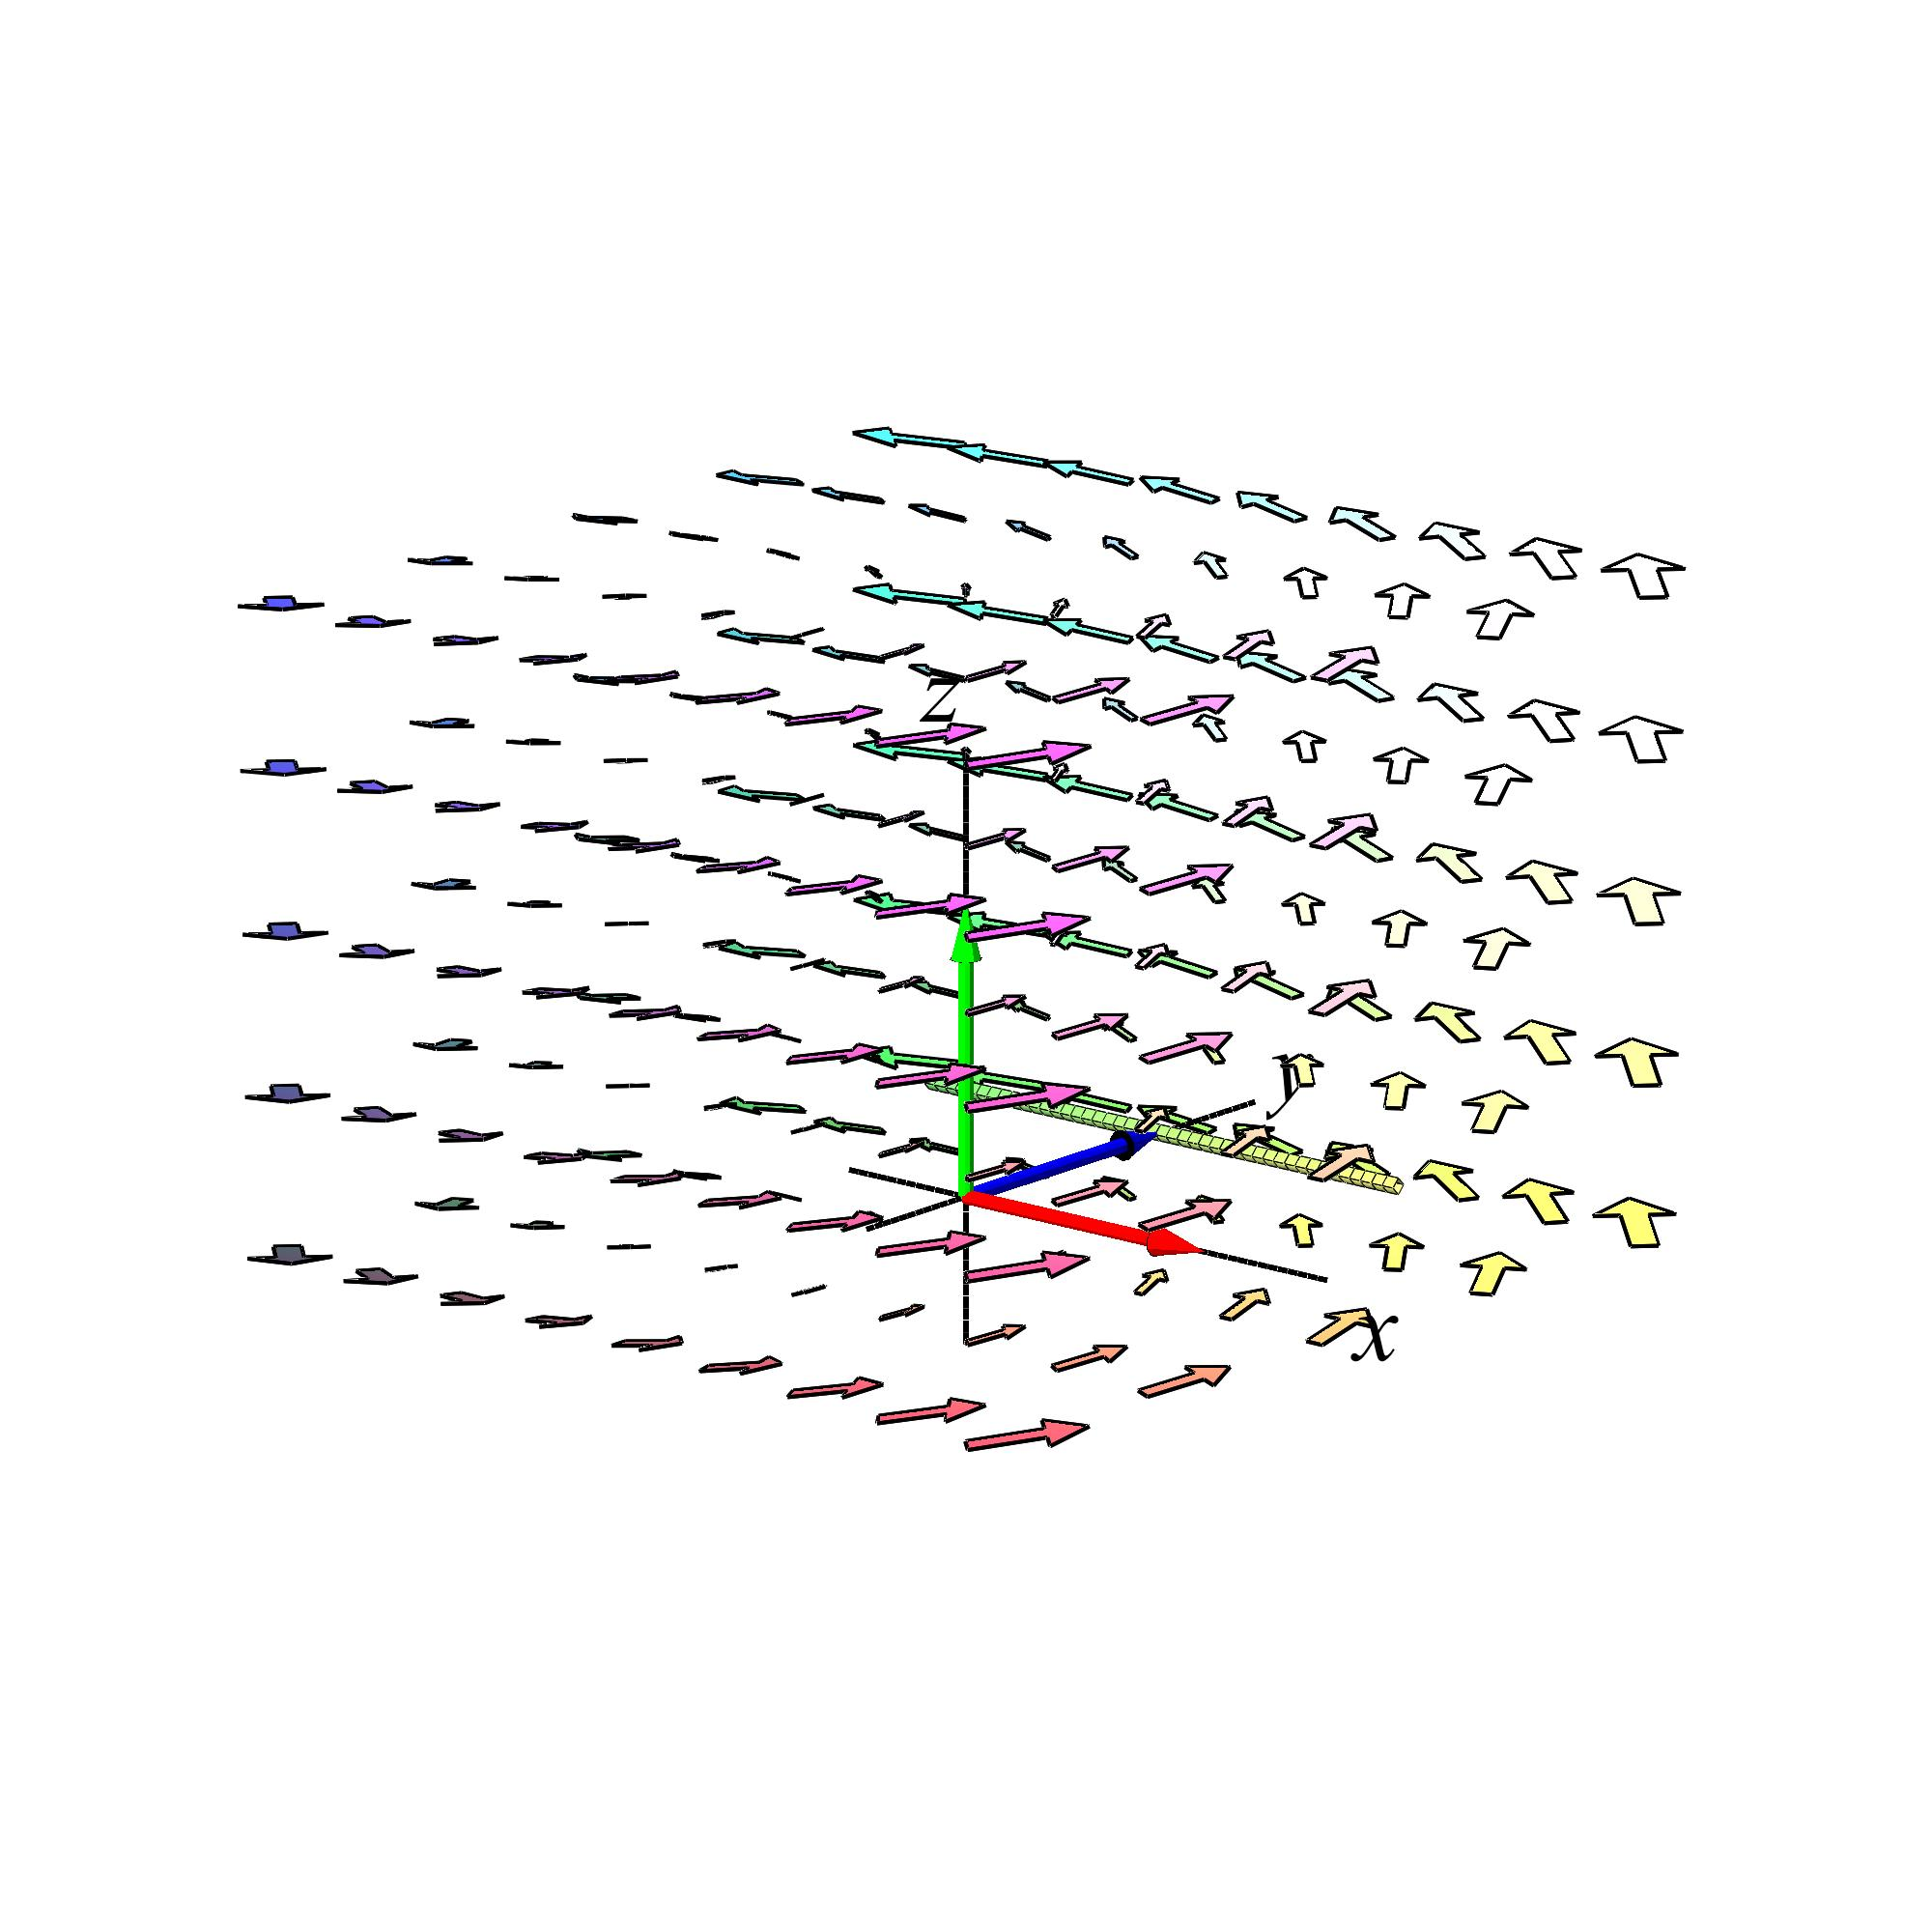
\includegraphics[height=70mm]{FIGS/plotVFkurveflow1}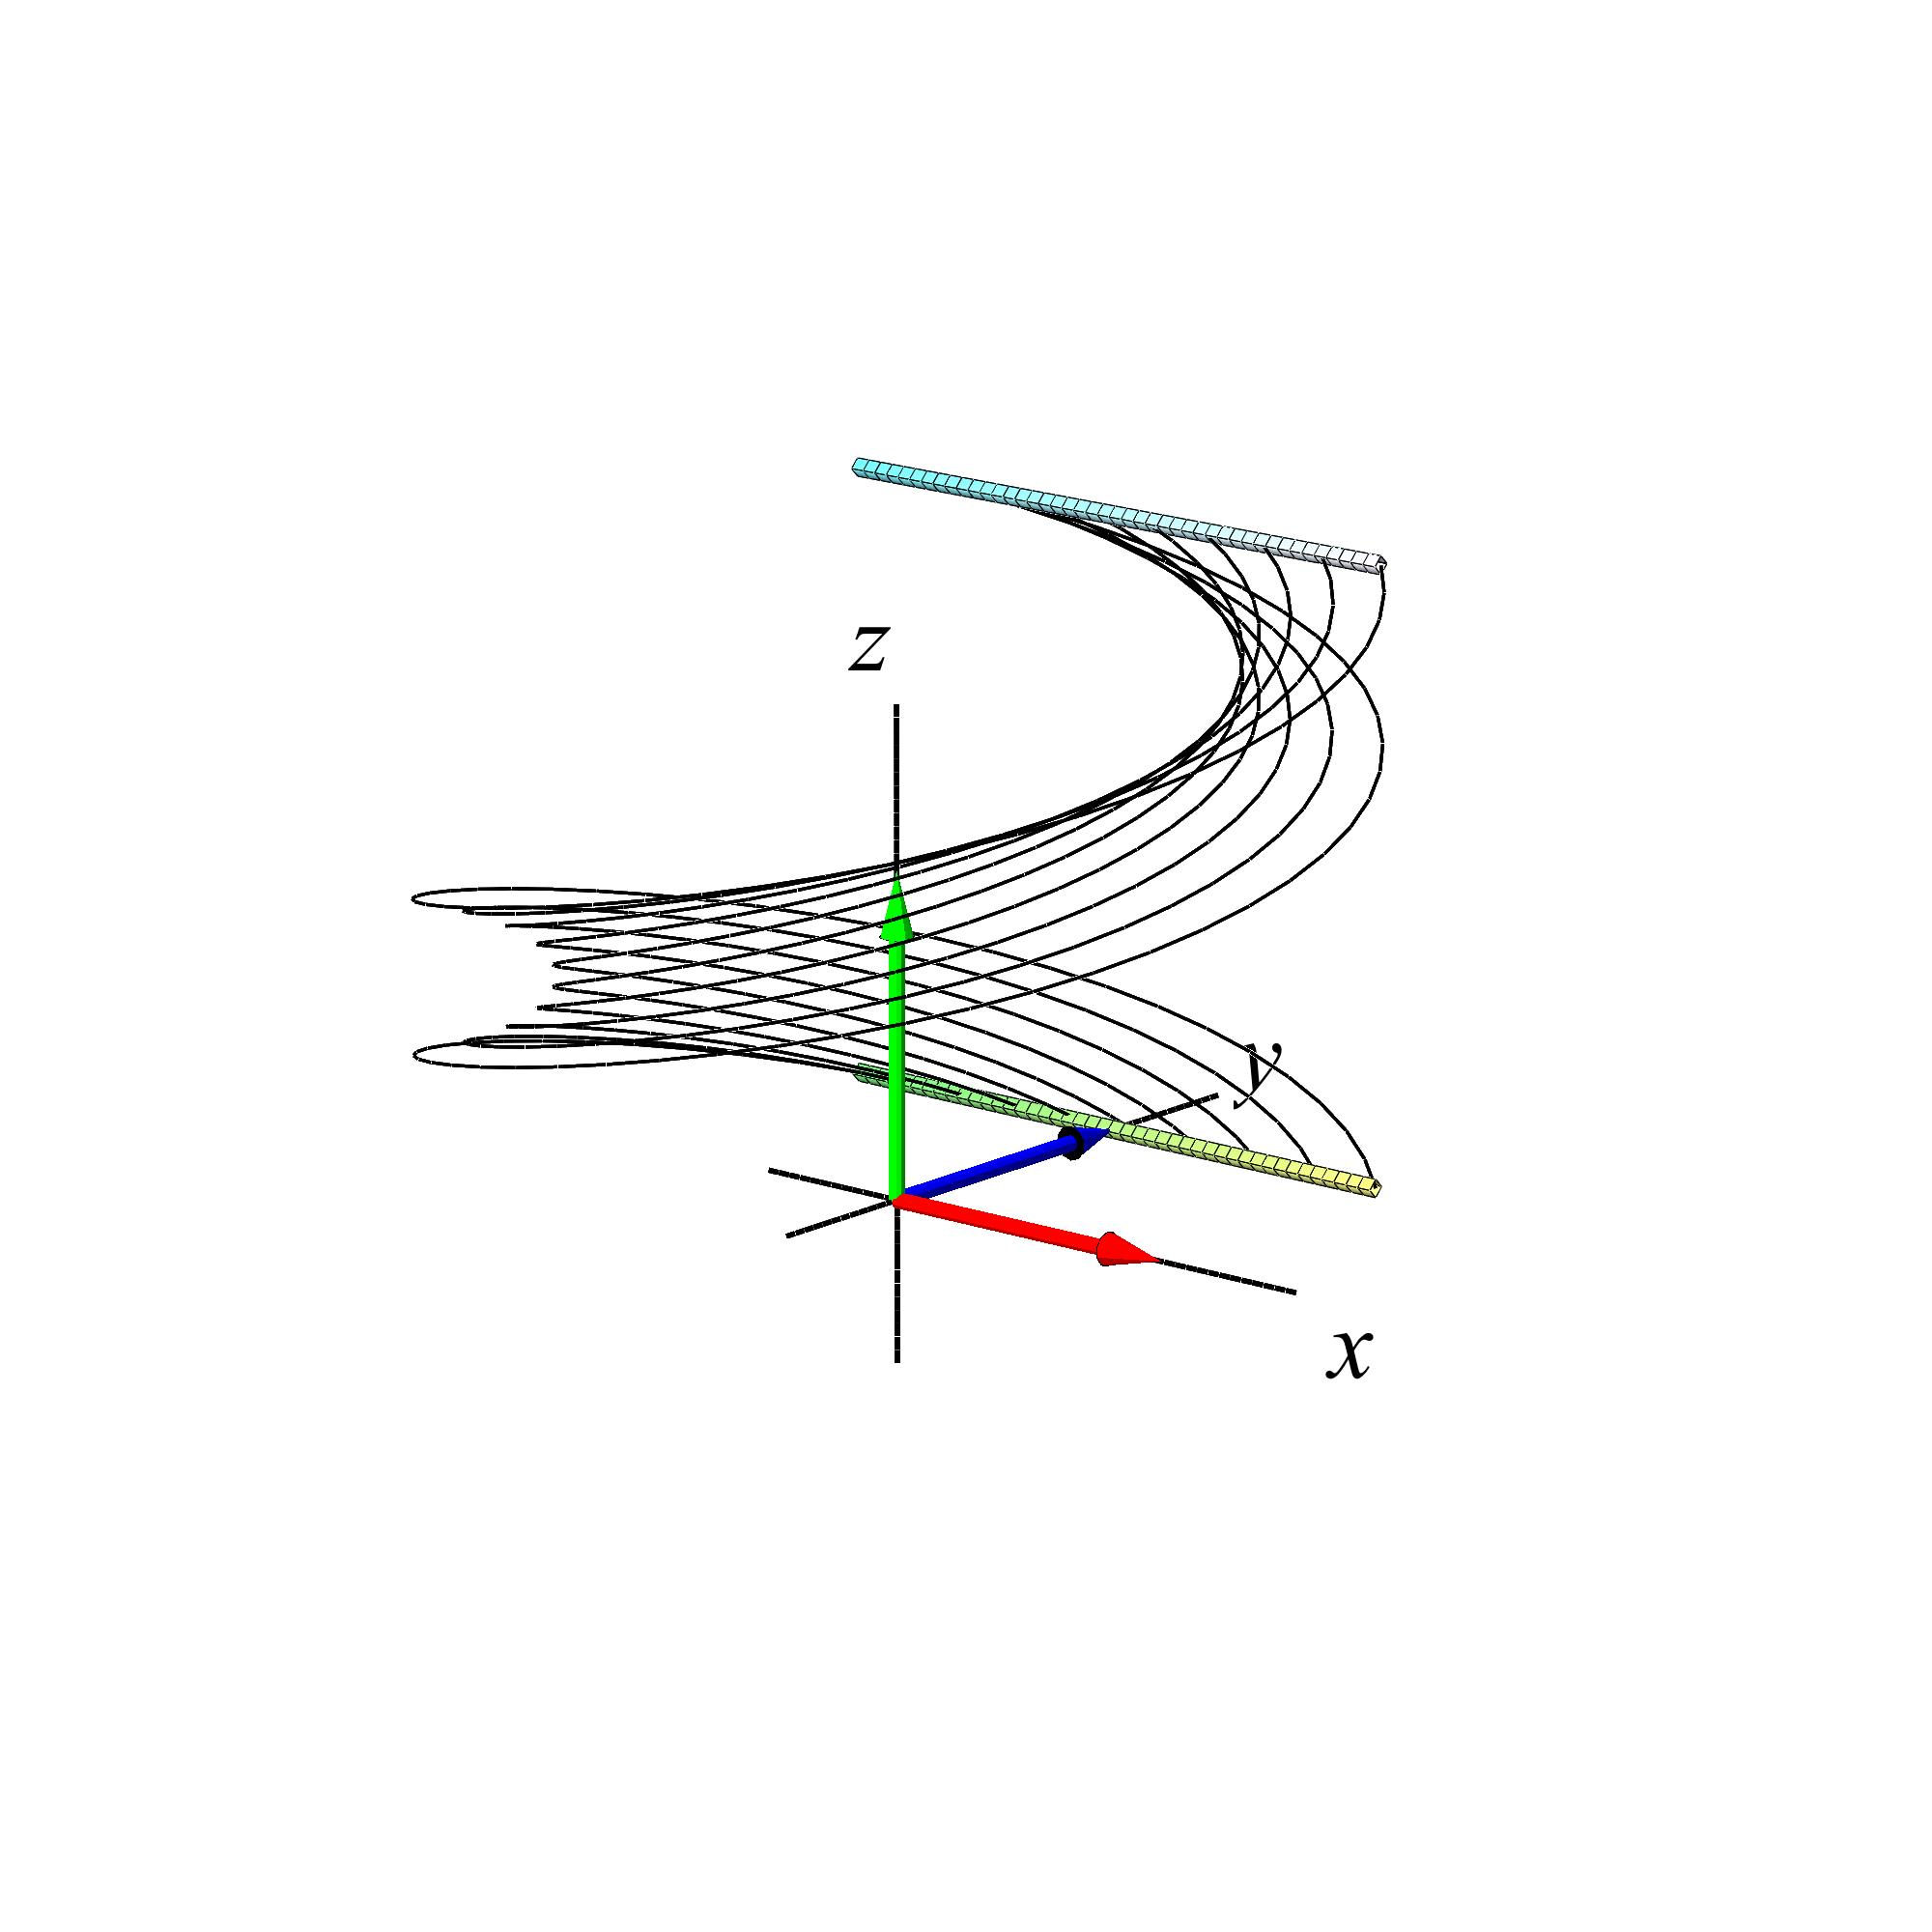
\includegraphics[height=70mm]{FIGS/plotVFkurveflow2}}
\begin{center}
\caption{\small{Et linjestykke flyder med flowkurverne for vektorfeltet $\mathbf{V}(x,y,z)= (-y, x, 0.3)$.}}
\label{figVFKurveFlow}
\end{center}
\end{figure}

\begin{figure}[h]
\centerline{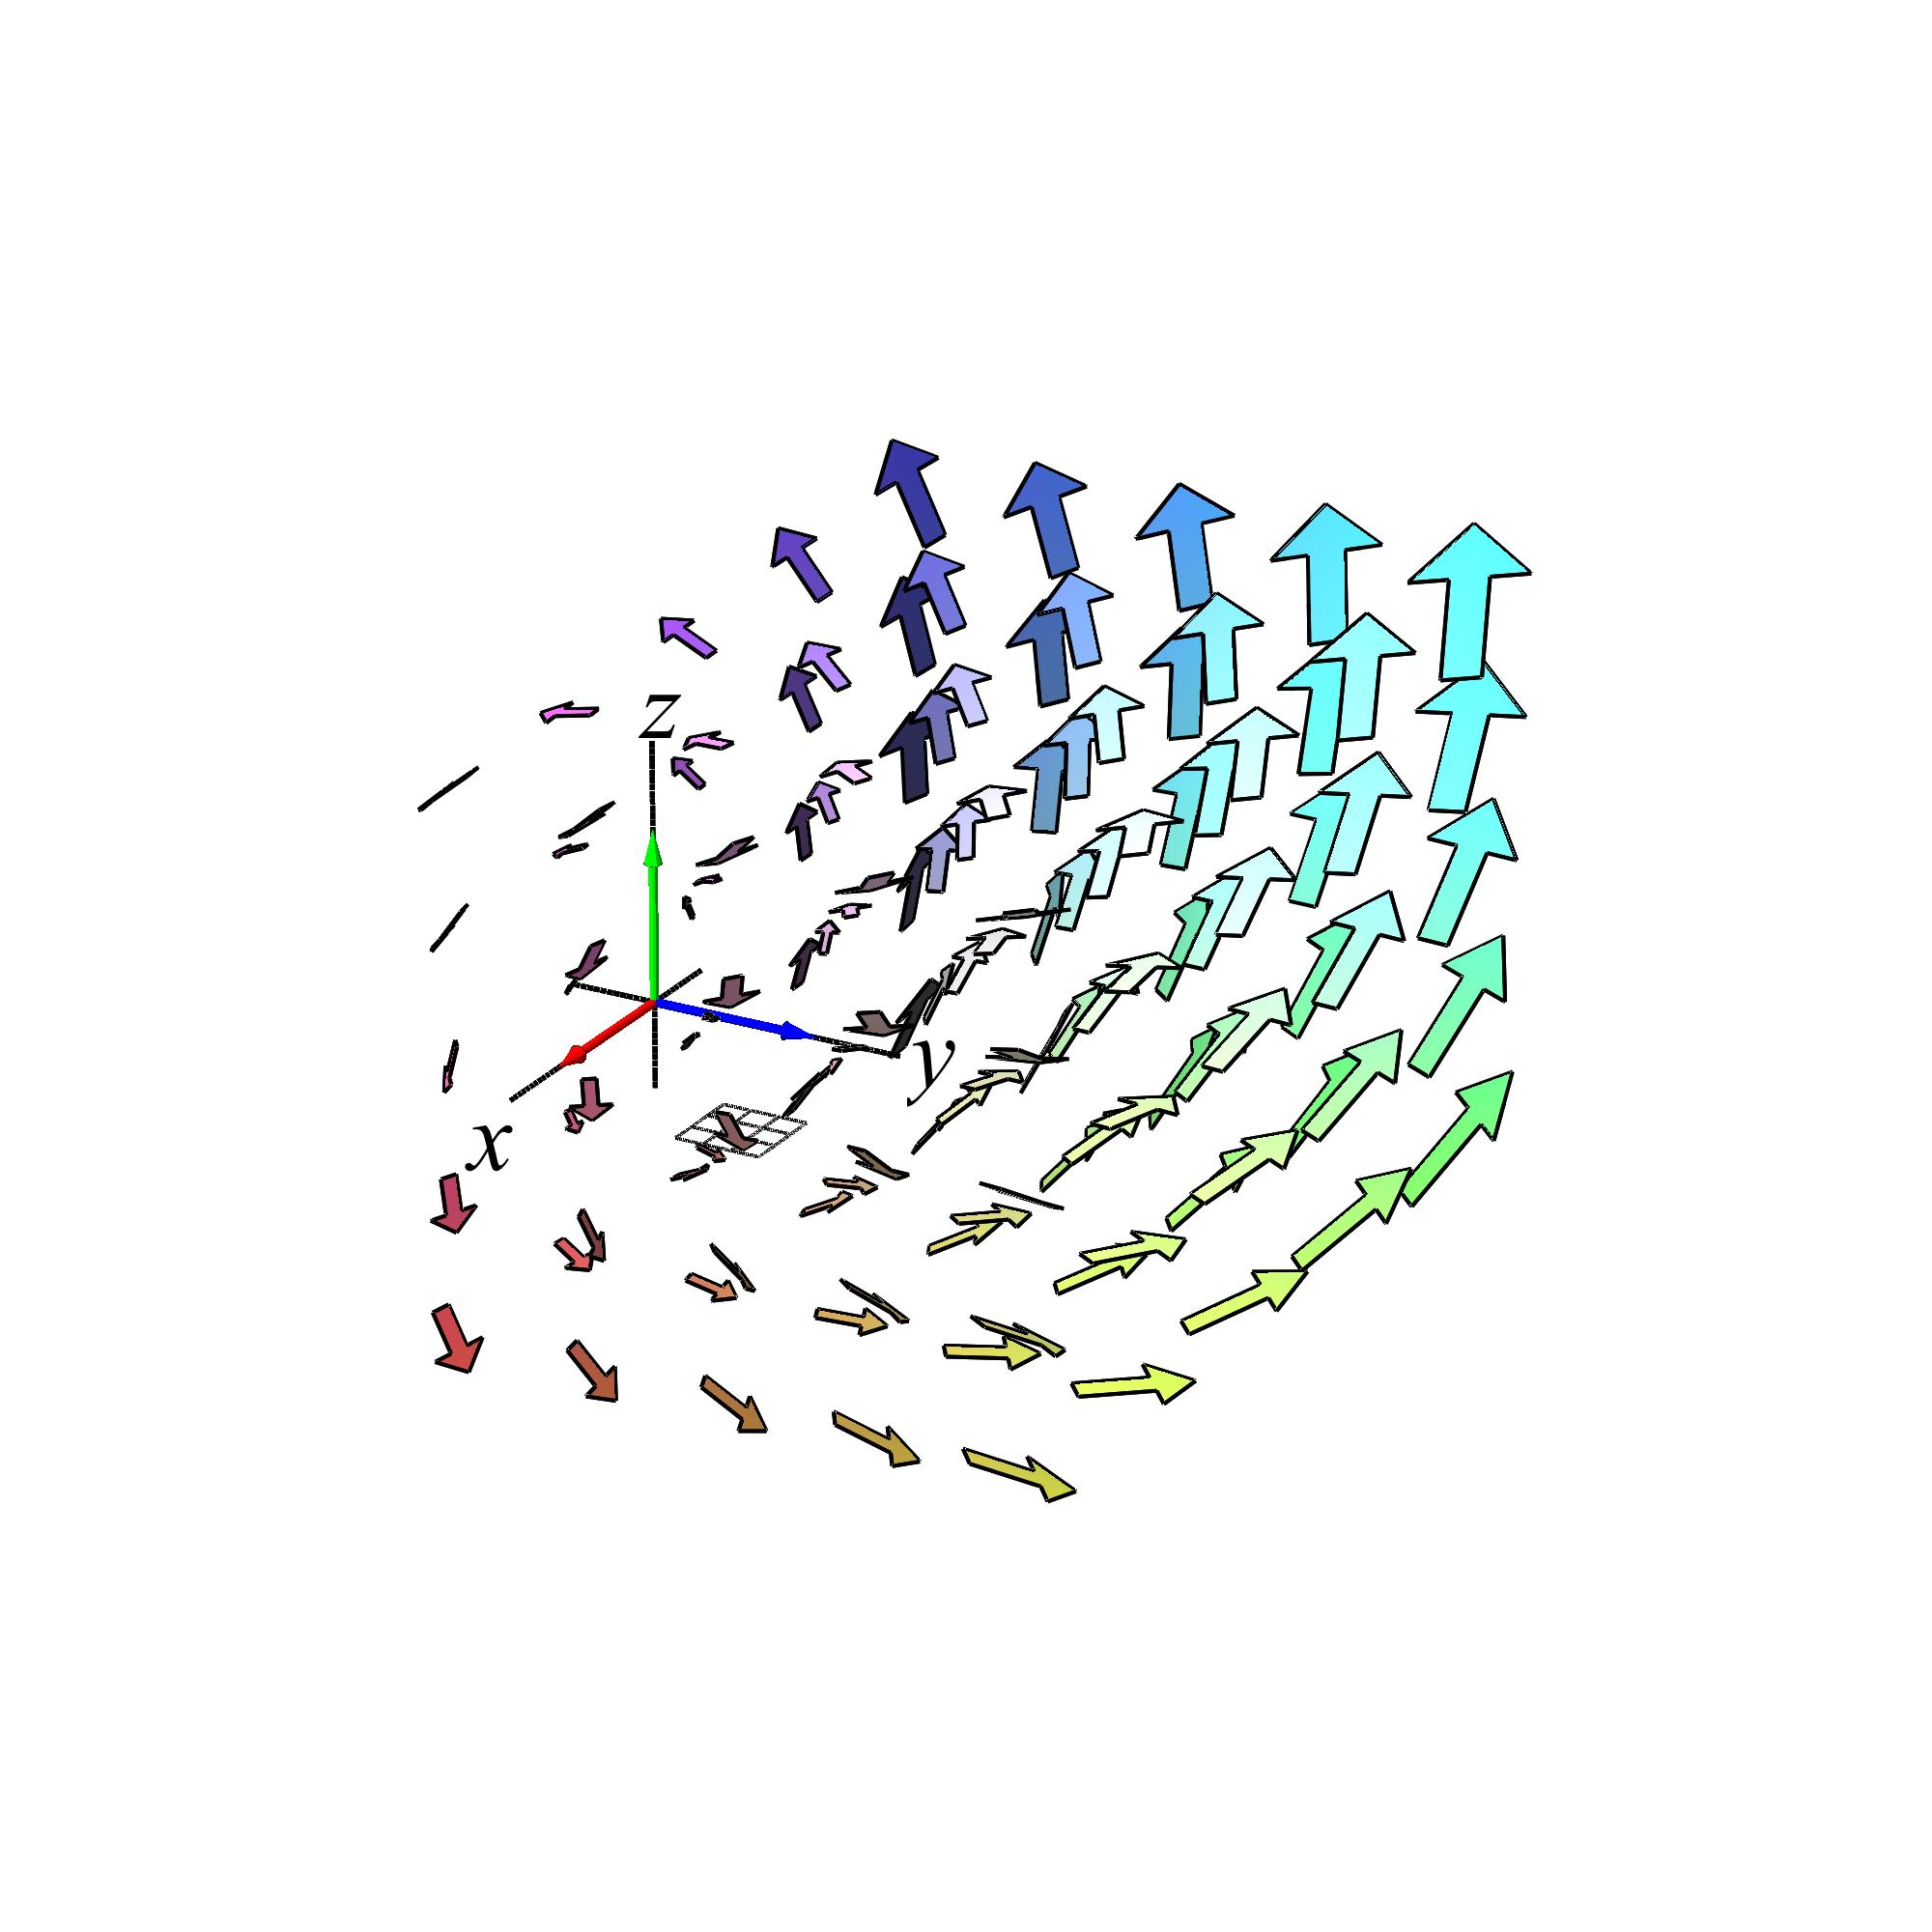
\includegraphics[height=70mm]{FIGS/plotVFfladeflow1}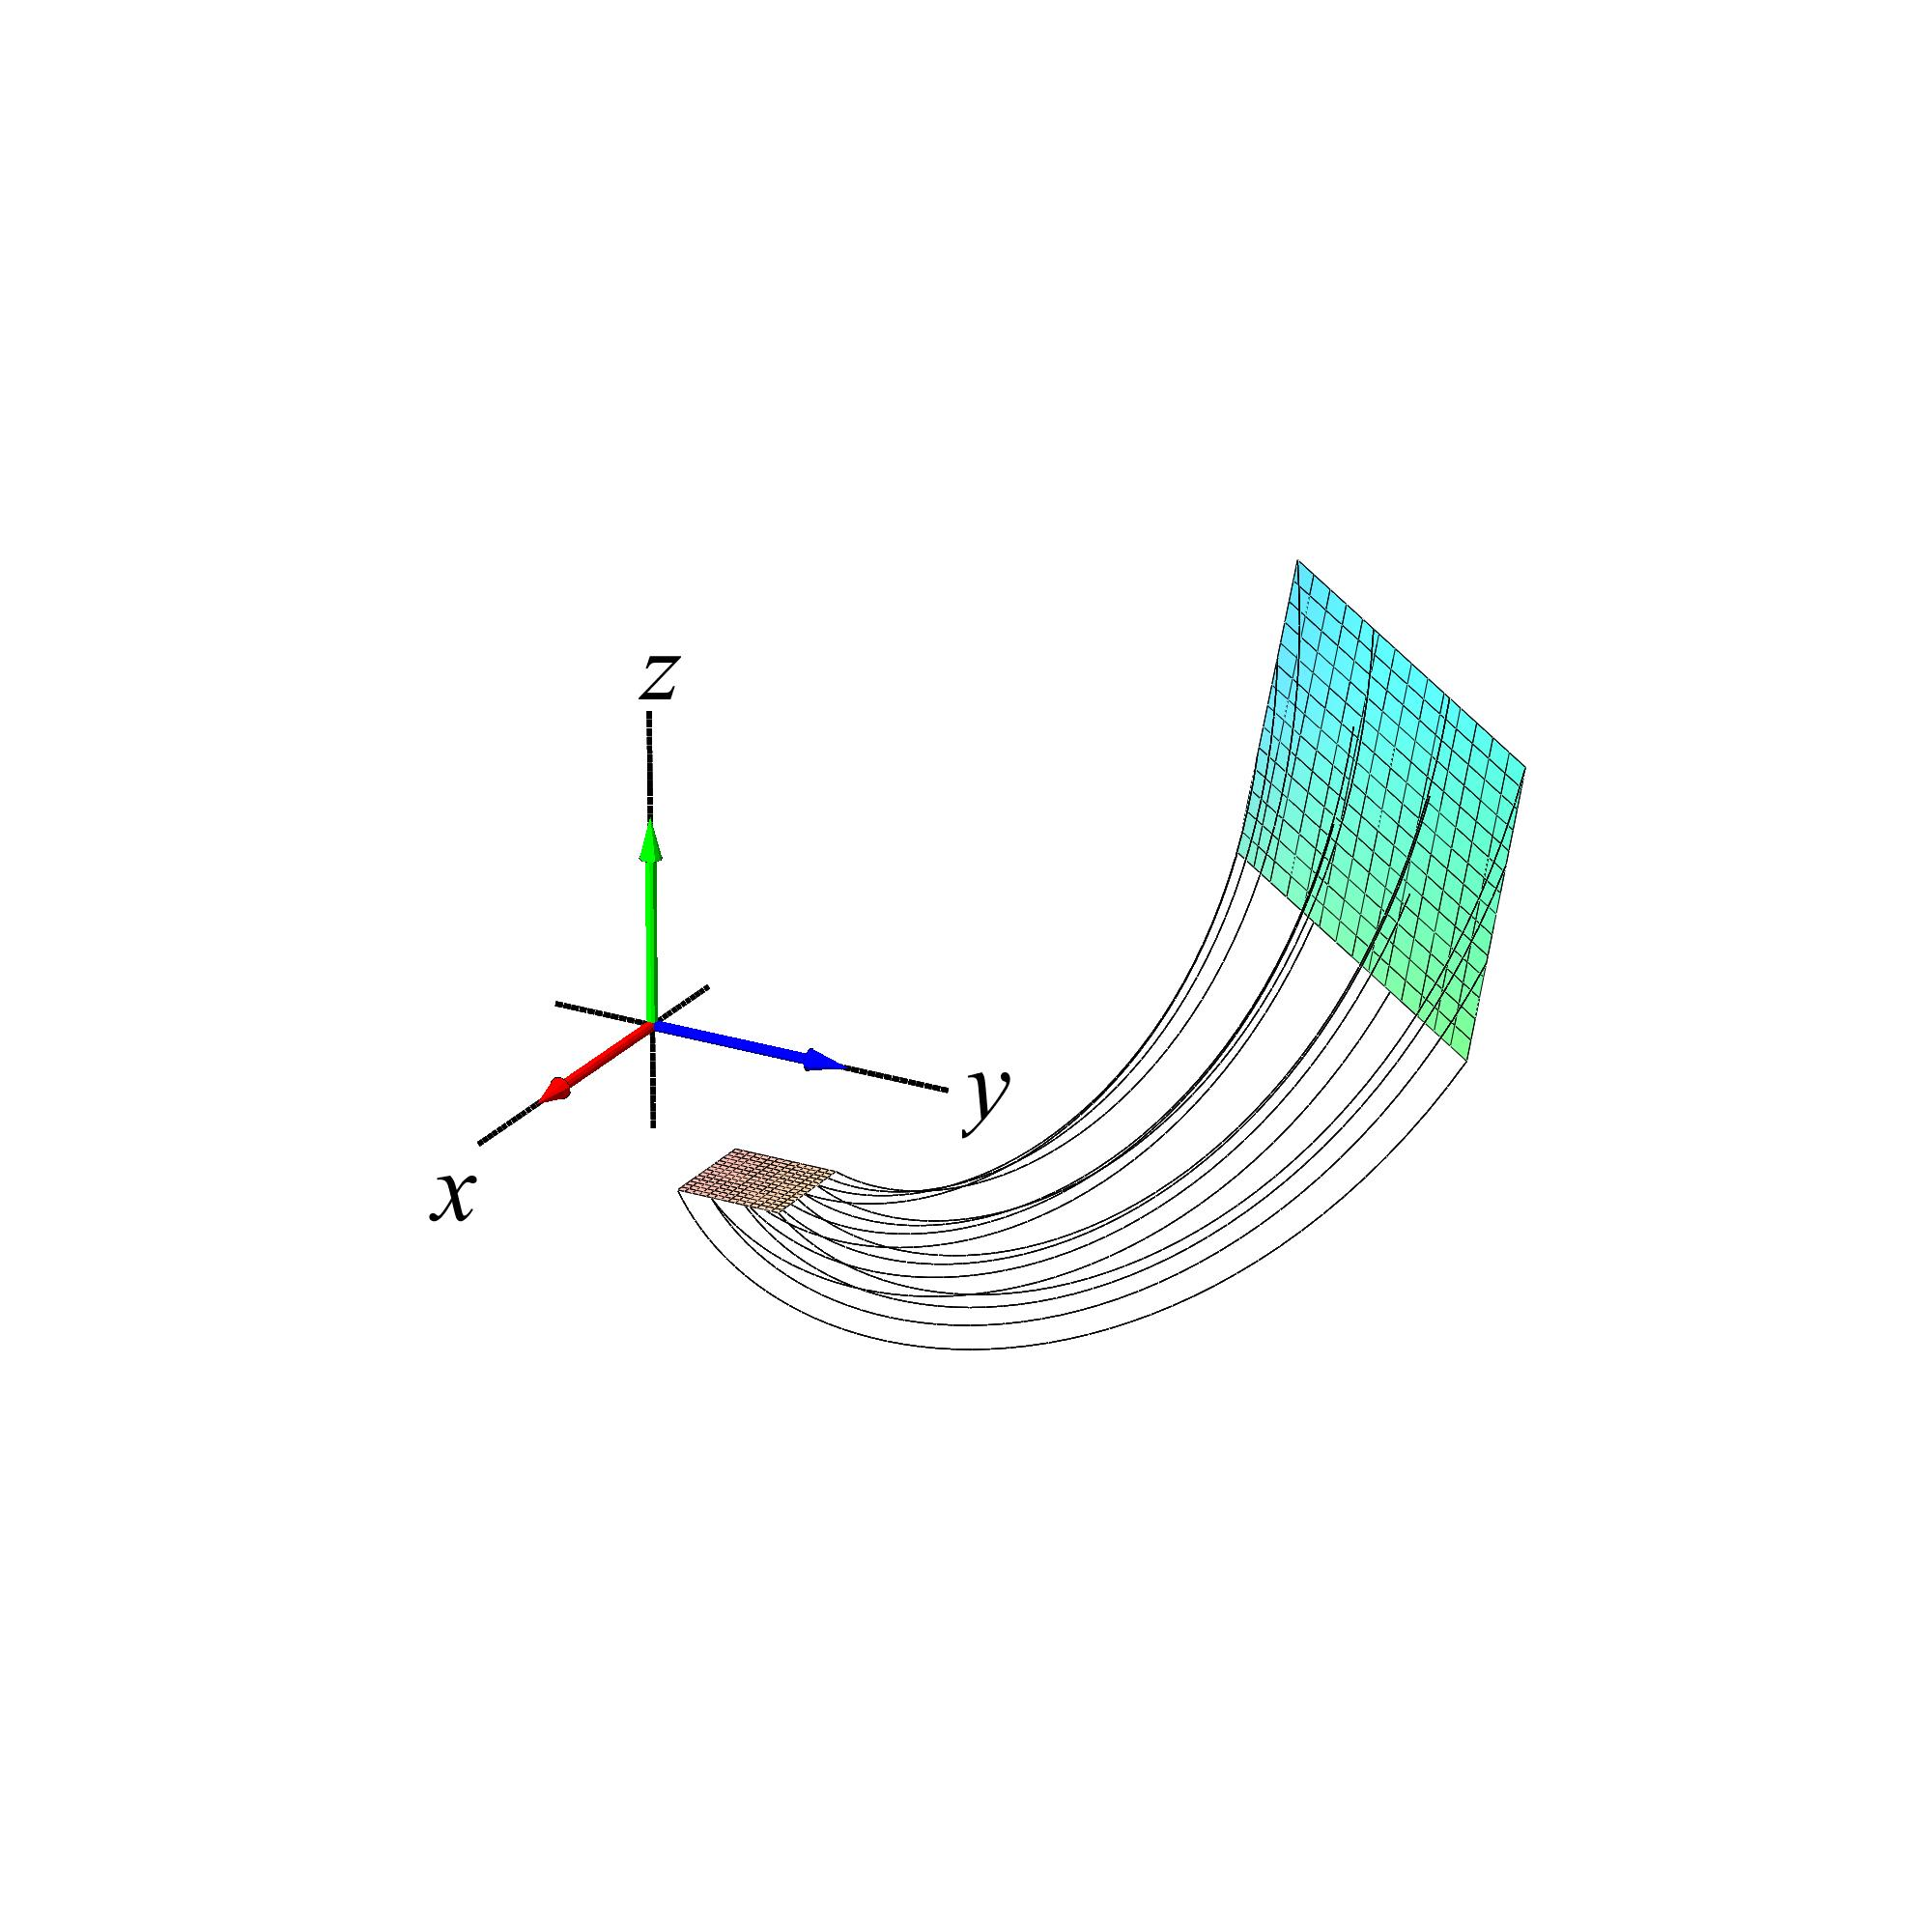
\includegraphics[height=70mm]{FIGS/plotVFfladeflow2}}
\begin{center}
\caption{\small{Et kvadrat flyder med flowkurverne for vektorfeltet $\mathbf{V}(x,y,z)= (-y + (x/9), -z+(y/9), -x + (z/9))$.}}
\label{figVFfladeFlow}
\end{center}
\end{figure}


\subsection{Flow af niveaukurver og niveauflader} \label{secLevelFlow}
Gradientvektorfelterne for funktioner af to og tre variable deformerer også kurver og flader via de respektive flowkurver.
Man kunne nu forledes til at  tænke, at niveaukurver og niveauflader nok flyder over i andre niveaukurver og niveauflader ved gradientvektorflowet. Så simpelt er det ikke -- men næsten.

\begin{think}
Ved nærmere eftertanke vil man indse, at det heller ikke kan være rigtigt at gradientvektorfeltet generelt skulle flyde niveaumængder i niveaumængder. Hvis f.eks. to nabo-niveaukurver i figur \ref{figGradFelt} ligger tæt på hinanden,  så er gradientvektoren tilsvarende stor og omvendt hvis to nabo-niveaukurver ligger længere fra hinanden,  så er gradientvektoren tilsvarende mindre. Dvs. der hvor gradienvektorerne er store skal vi flyde langsomt og der for de er små skal vi flyde hurtigt for at niveaukurverne kan flyde over i hinanden.
\end{think}


\begin{theorem}[Niveau-mængde flow] \label{thmLevelFlow}
Lad $f(x,y,z)$ betegne en glat funktion af tre variable med et egentligt gradientvektorfelt $\bm{\nabla}f(x,y,z) \neq \mathbf{0}$.
Lad $\mathbf{V}(x,y,z)$ være det kvadratisk normerede gradientvektorfelt:
\begin{equation}
\mathbf{V}(x,y,z) = \frac{\bm{\nabla}f(x,y,z)}{|\, \bm{\nabla}f(x,y,z)\,|^{2}} \quad .
\end{equation}
Hvis vi lader ethvert punkt $p$ på niveaufladen $\mathcal{K}_{c}(f)$ flyde tiden $t_{0}$ med den flowkurve for $\mathbf{V}(x,y,z)$ som starter i $p$, så vil hele niveaufladen flyde over i niveaufladen $\mathcal{K}_{c+t_{0}}(f)$.\\

Et tilsvarende resultat gælder  for gradientvektorfelter for glatte funktioner $f(x,y)$ af to variable og deres tilhørende niveaukurver i planen.
\end{theorem}
\begin{bevis}
Vi skal bare vise, at hvis vi starter (til tiden $t=0$) i et punkt $p$ hvor $f(p) = c$ så lander vi med flowkurven $\mathbf{r}(t)$ for vektorfeltet $\mathbf{V}(x,y,z)$ efter tiden $t_{0}$ i et punkt $\mathbf{r}(t_{0})$ hvor $f(x,y,z)$ har værdien $f(\mathbf{r}(t_{0})) = c + t_{0}$. \\

 Vi bruger kædereglen for tilvæksten af funktionsværdier langs en flowkurve, se \tref{NUID28-tn15}{eNote}:
\begin{equation} \label{eqChainFlow}
\frac{d}{dt}f(\mathbf{r}(t)) = \bm{\nabla}f(\mathbf{r}(t)) \bm{\cdot} \mathbf{r}'(t) \quad ,
\end{equation}
og da $\mathbf{r}(t)$ er en flowkurve for $\mathbf{V}(x,y,z)$ ved vi, at $\mathbf{r}'(t) = \mathbf{V}(\mathbf{r}(t))$ som indsat i (\ref{eqChainFlow}) giver:
\begin{equation}
\begin{aligned}
\frac{d}{dt}f(\mathbf{r}(t)) &= \bm{\nabla}f(\mathbf{r}(t)) \bm{\cdot} \mathbf{V}(\mathbf{r}(t)) \\
&= \bm{\nabla}f(\mathbf{r}(t)) \bm{\cdot} \frac{\bm{\nabla}f(\mathbf{r}(t))}{|\, \bm{\nabla}f(\mathbf{r}(t))\,|^{2}}  \\
& = \frac{\bm{\nabla}f(\mathbf{r}(t)) \bm{\cdot} \bm{\nabla}f(\mathbf{r}(t))}{|\, \bm{\nabla}f(\mathbf{r}(t))\,|^{2}}  \\
&= 1 \quad .
\end{aligned}
\end{equation}
Heraf fås det ønskede direkte:
\begin{equation}
\begin{aligned}
f(\mathbf{r}(t_{0})) &= c + \int_{0}^{t_{0}} \frac{d}{dt}f(\mathbf{r}(t)) \, dt \\
&= c + \int_{0}^{t_{0}} 1 \, dt \\
&= c + t_{0} \quad .
\end{aligned}
\end{equation}
\end{bevis}


%%%%%%%%%%%%%%%%%%%%%%%%%%%%%%%%%%%%%%%%%%%%%%%%%%%%%%%%%%%%%
%%%%%%%%%%%%%%%%%%%%%%%%%%%%%%%%%%%%%%%%%%%%%%%%%%%%%%%%%%%%%
%%%%%%%%%%%%%%%%%%%%%%%%%%%%%%%%%%%%%%%%%%%%%%%%%%%%%%%%%%%%%

\begin{summary}
Vi har i denne eNote etableret de første begreber og metoder til analyse af vektorfelter i plan og rum.
\begin{itemize}
\item Nogle men ikke alle vektorfelter fremkommer som gradientvektorfelter for funktioner $f(x,y,z)$ (her af tre variable):
\begin{equation}
\bm{\nabla}f(x,y,z) = \left(f'_{x}(x,y,z)\, , \, f'_{y}(x,y,z) \, , \, f'_{z}(x,y,z)\right) \quad , \quad (x,y,z) \in \mathbb{R}^{3} \quad .
\end{equation}
\item Ethvert vektorfelt $\mathbf{V}(x,y,z)$ af første grad kan skrives og angives ved hjælp af en systemmatrix $\mathbf{A}$ og en konstant vektor $\mathbf{b}$:
\begin{equation}
\left[
  \begin{array}{c}
    V_{1}(x,y,z) \\
    V_{2}(x,y,z) \\
    V_{3}(x,y,z) \\
  \end{array}\right] \, = \, \left[
                        \begin{array}{ccc}
                          a_{11} & a_{12} & a_{13} \\
                          a_{21} & a_{22} & a_{23} \\
                          a_{31} & a_{32} & a_{33} \\
                        \end{array}\right]\cdot \left[
                                        \begin{array}{c}
                                          x \\
                                          y \\
                                          z \\
                                        \end{array}
                                      \right] \, + \, \left[
                                                        \begin{array}{c}
                                                          b_{1} \\
                                                          b_{2} \\
                                                          b_{3} \\
                                                        \end{array}
                                                      \right] \quad .
\end{equation}
\item For at forstå geometrien af et givet vektorfelt er det vigtigt at kunne bestemme vektorfeltets flow-kurver -- det er de parametriserede kurver $\mathbf{r}(t) = (x(t), y(t), z(t))$, $t\in [a,b]$, som i alle kurve-punkter har det givne vektorfelt som tangentvektor. Hvis vektorfeltet er givet ved $\mathbf{V}(x,y,z) = (V_{1}(x,y,z), V_{2}(x,y,z), V_{3}(x,y,z))$, så er flowkurve-ligningen:
\begin{equation}
\left[
  \begin{array}{c}
    x'(t) \\
    y'(t) \\
    z'(t) \\
  \end{array}
\right] = \left(\mathbf{V}(x(t), y(t), z(t))\right)^{\top} = \left[
                                                  \begin{array}{c}
                                                    V_{1}(x(t), y(t), z(t)) \\
                                                     V_{2}(x(t), y(t), z(t)) \\
                                                     V_{3}(x(t), y(t), z(t)) \\
                                                  \end{array}
                                                \right] \quad .
\end{equation}
\item Divergensen af et vektorfelt $\mathbf{V}(x,y,z)$ har vi defineret som den funktion, der i et vilkårligt punkt $(x_{0}, y_{0}, z_{0})$ har værdien:
\begin{equation}
\operatorname{Div}({\mathbf{V}})(x_{0},y_{0},z_{0}) \, = \,
\frac{\partial V_{1}}{\partial
x}(x_{0},y_{0},z_{0}) + \frac{\partial
V_{2}}{\partial y}(x_{0},y_{0},z_{0}) +
\frac{\partial V_{3}}{\partial
z}(x_{0},y_{0},z_{0}) \quad ,
\end{equation}
og vi har antydet med meget simple eksempler, at divergensen er et lokalt  mål for hvor meget vektorfeltet spreder eller samler  en given mængde af partikler, der flyder med vektorfeltet, dvs. følger vektorfeltets flowkurver.
\item Rotationen af et vektorfelt har vi defineret som følgende vektorfelt
\begin{equation}
\begin{aligned}
\operatorname{\mathbf{Rot}}({\mathbf{V}})(x_{0},y_{0},z_{0}) \, = \, \Large{(} \, \,  &\frac{\partial
V_{3}}{\partial y}(x_{0},y_{0},z_{0}) - \frac{\partial
V_{2}}{\partial z}(x_{0},y_{0},z_{0})\, , \\
&\frac{\partial V_{1}}{\partial z}(x_{0},y_{0},z_{0}) -
\frac{\partial
V_{3}}{\partial x}(x_{0},y_{0},z_{0})\, , \\
&\frac{\partial V_{2}}{\partial x}(x_{0},y_{0},z_{0}) -
\frac{\partial V_{1}}{\partial y}(x_{0},y_{0},z_{0})\,\,  \Large{)} \quad ,
\end{aligned}
\end{equation}
og vi har antydet med meget simple eksempler, at rotationen er et lokalt  mål for hvor meget vektorfeltet roterer en given mængde af partikler, der flyder med vektorfeltet dvs. følger vektorfeltets flowkurver.
\end{itemize}
\end{summary}


%%%%%%%%%%%%%%%%%%%%%%%%%%%%%%%%%%%%%%%%%%%%%
%%%%%%%%%%%%%%%%%%%%%%%%%%%%%%%%%%%%%%%%%%%%%
%%% HER SKAL DU STOPPE MED AT SKRIVE %%%%%%%%
%%%%%%%%%%%%%%%%%%%%%%%%%%%%%%%%%%%%%%%%%%%%%
%%%%%%%%%%%%%%%%%%%%%%%%%%%%%%%%%%%%%%%%%%%%%


\end{document} 

%%%%%%%%%%%%%%%%%%%%%%%%%%%%%%%%%%%%%%%%%%%%%%%%%%%
%%%%%%%%%%%%%%%%%%%%%%%%%%%%%%%%%%%%%%%%%%%%%%%%%%%

